%APPENDI
\chapter{$Z\gamma$ FSR and ISR Plots}
\label{sec:ZgFSRandISRplots}

Data sample selected in $Z\gamma\rightarrow\mu\mu\gamma$ conditions where photon selection is the same as for $W\gamma$ selection is used to prepare real-$\gamma$ and fake-$\gamma$ templates for the jets$\rightarrow\gamma$ background estimation. The nominal $Z\gamma$ events selection is described in Ch.~\ref{sec:AN_Selection_EventLevel}, and we considered four variables to introduce changes to the nominal selection to increase either real-$\gamma$ or fake-$\gamma$ fractions: the three-particle invariant mass $M_{\mu\mu\gamma}$, the invariant mass of the dimuon system $M_{\mu\mu}$ (Fig.~\ref{fig:Zg_Mleplep_and_Mpholeplep}), the separations between muons and the photon $\Delta{R}(\mu_1,\gamma)$, $\Delta{R}(\mu_2,\gamma)$ (Fig.~\ref{fig:Zg_ISRandFSR_dR}), where $\mu_1$ is the muon with the smaller separation from the photon out of two muons in the given candidate. 

The two peaks in the $M_{\mu\mu\gamma}$ and $M_{\mu\mu}$ distributions correspond to FSR and ISR mechanisms of the $Z\gamma$ production, where FSR peak is highly dominated by real-$\gamma$ events, and ISR peak contains a significant number of both $Z\gamma$ and DY+jets events. It is also seen in Fig.~\ref{fig:Zg_ISRandFSR_dR} that events with smaller separation $\Delta{R}(\mu_1,\gamma)$ have a larger fraction of $Z\gamma$ than events with the larger separation. The selection chosen to prepare real-$\gamma$ templates can be referred as FSR selection, while the selection chosen to prepare fake-$\gamma$ templates can be referred as ISR selection. The differences for the FSR and ISR selection from the nominal one are:
\begin{itemize}
  \item FSR: $M_{\mu\mu\gamma}<$101~GeV, $\Delta{R}(\mu_{1,2},\gamma)>$0.4;
  \item ISR: $M_{\mu\mu\gamma}>$101~GeV, $\Delta{R}(\mu_{1,2},\gamma)>$1.0.
\end{itemize}

The fake-$\gamma$ contribution into the FSR region is subtracted based on DY+jets MC predictions while the real-$\gamma$ contribution into the ISR region is subtracted based on $Z\gamma$ MC predictions. The number of real-$\gamma$ and fake-$\gamma$ events in different $P_T^\gamma$ bins is shown in Fig.~\ref{fig:Zg_ISRandFSR_phoEt}. The $I_{ch}^\gamma$ and $\sigma_{i \eta i \eta}^\gamma$ distributions are shown in Fig.~\ref{fig:Zg_FSR_phoPFChIsoCorr}-\ref{fig:Zg_ISR_phoSigmaIEtaIEta}.

\begin{figure}[htb]
  \begin{center}
   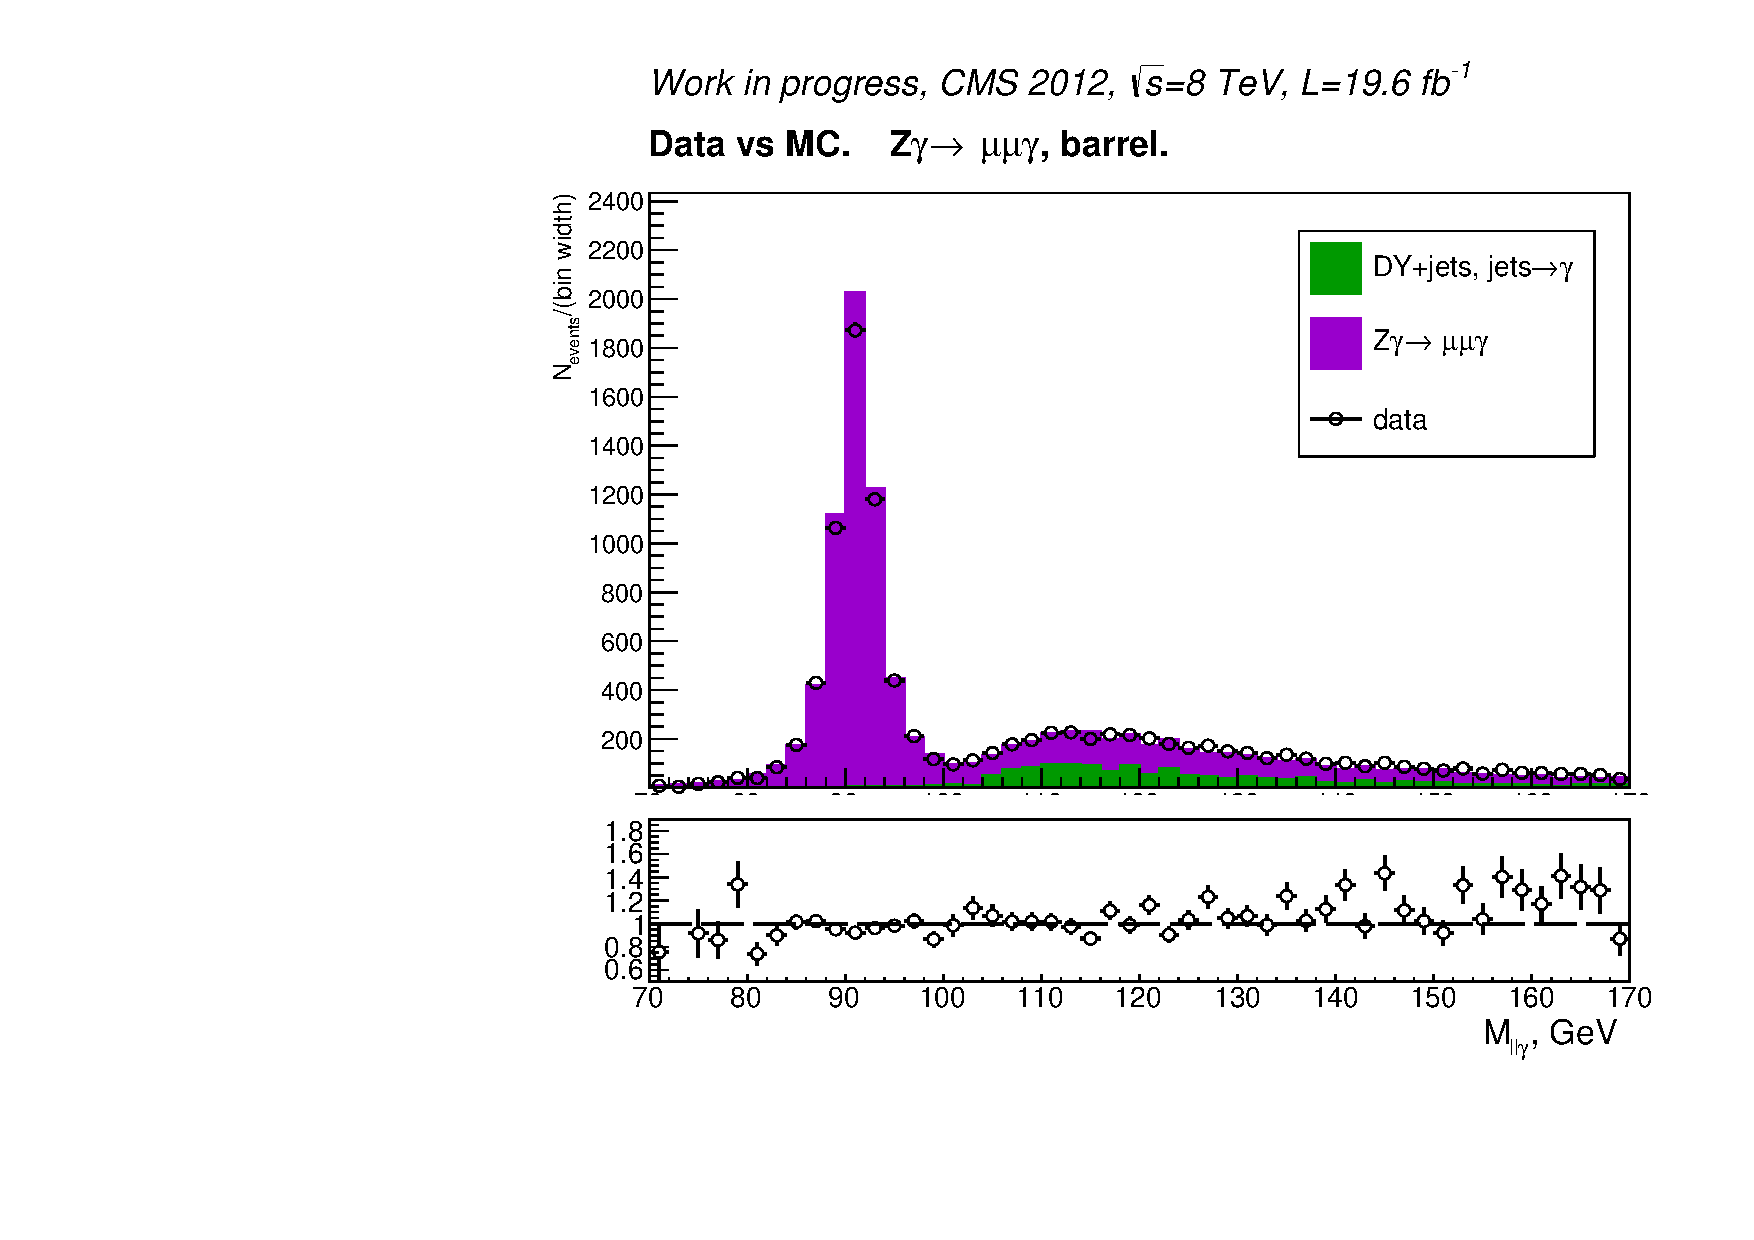
\includegraphics[width=0.45\textwidth]{../figs/figs_v11/MUON_ZGamma/PrepareYields/c_TotalDATAvsMC_Barrel__MpholeplepVERY_PRELIMINARY.pdf}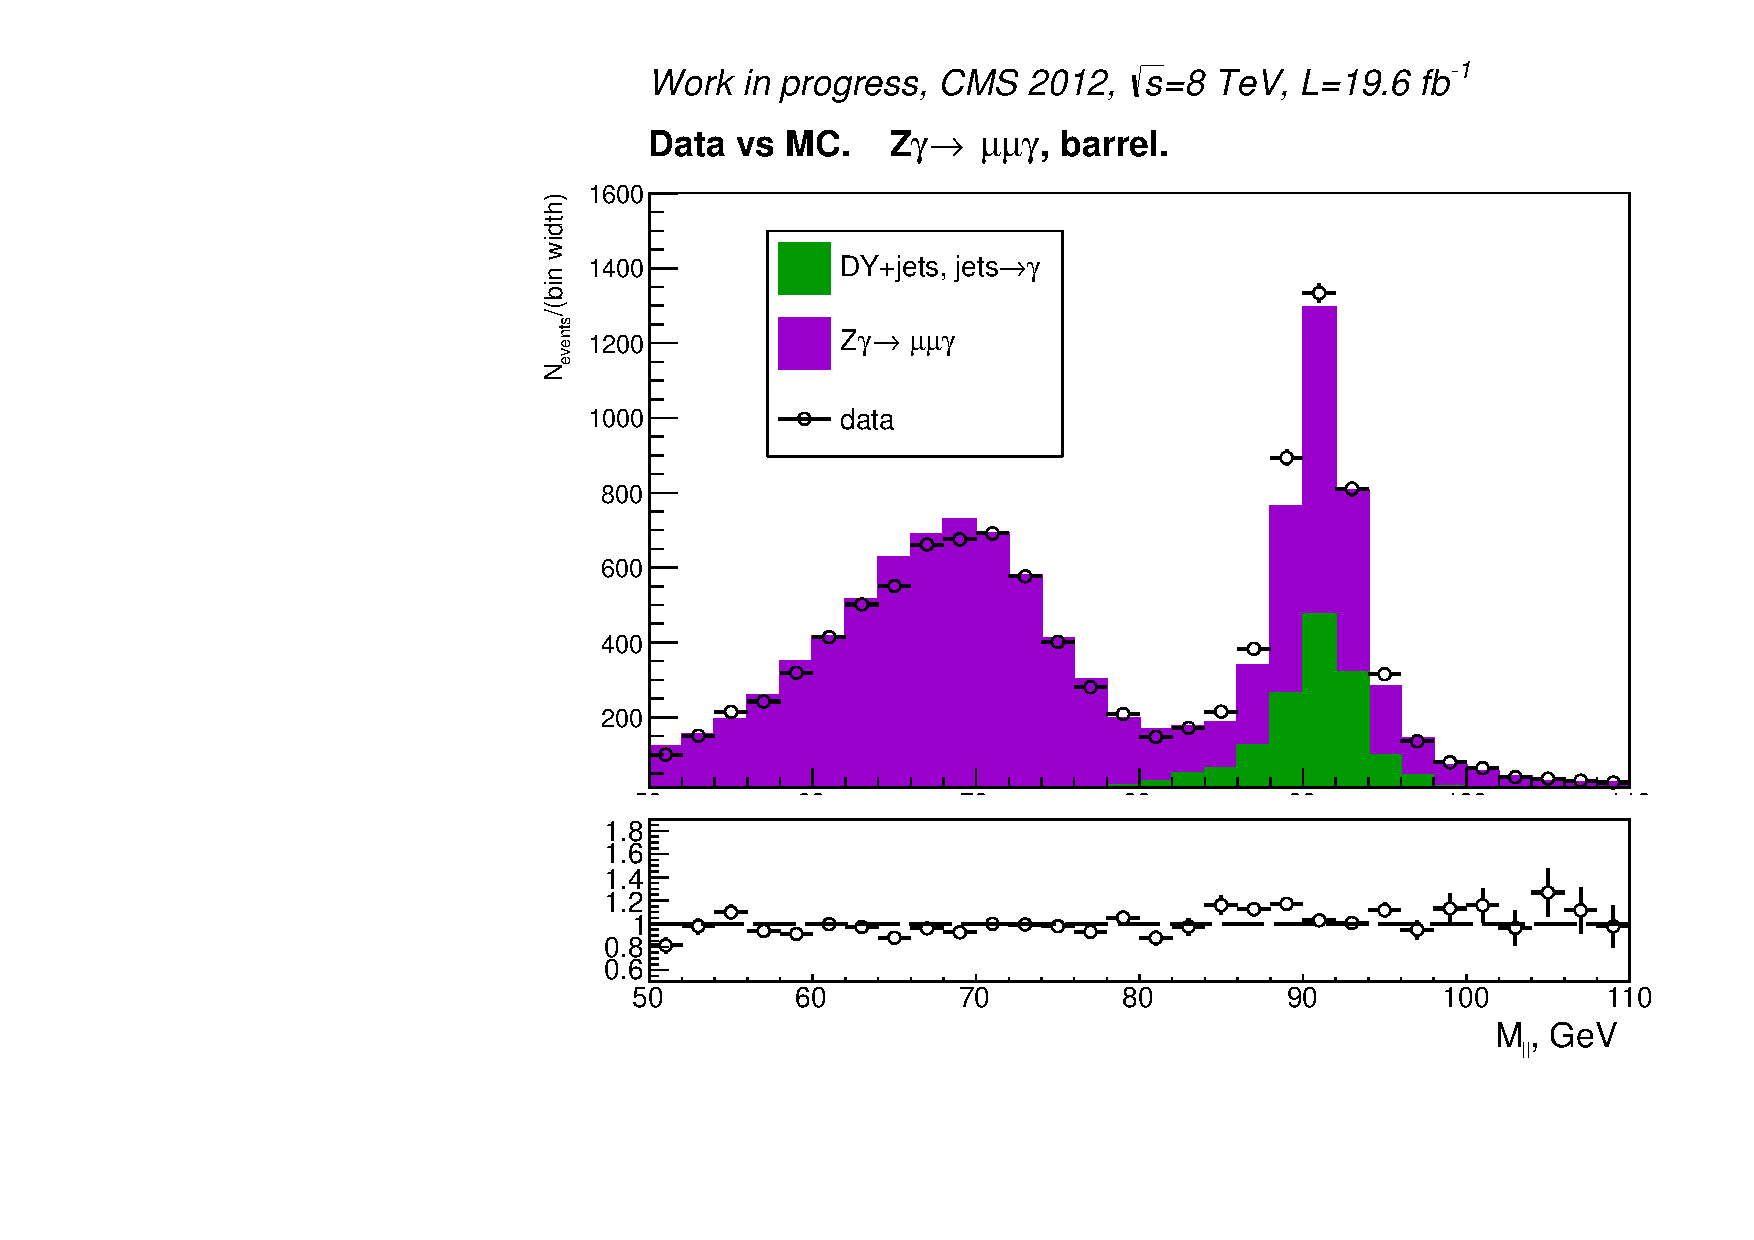
\includegraphics[width=0.45\textwidth]{../figs/figs_v11/MUON_ZGamma/PrepareYields/c_TotalDATAvsMC_Barrel__MleplepVERY_PRELIMINARY.pdf}\\
   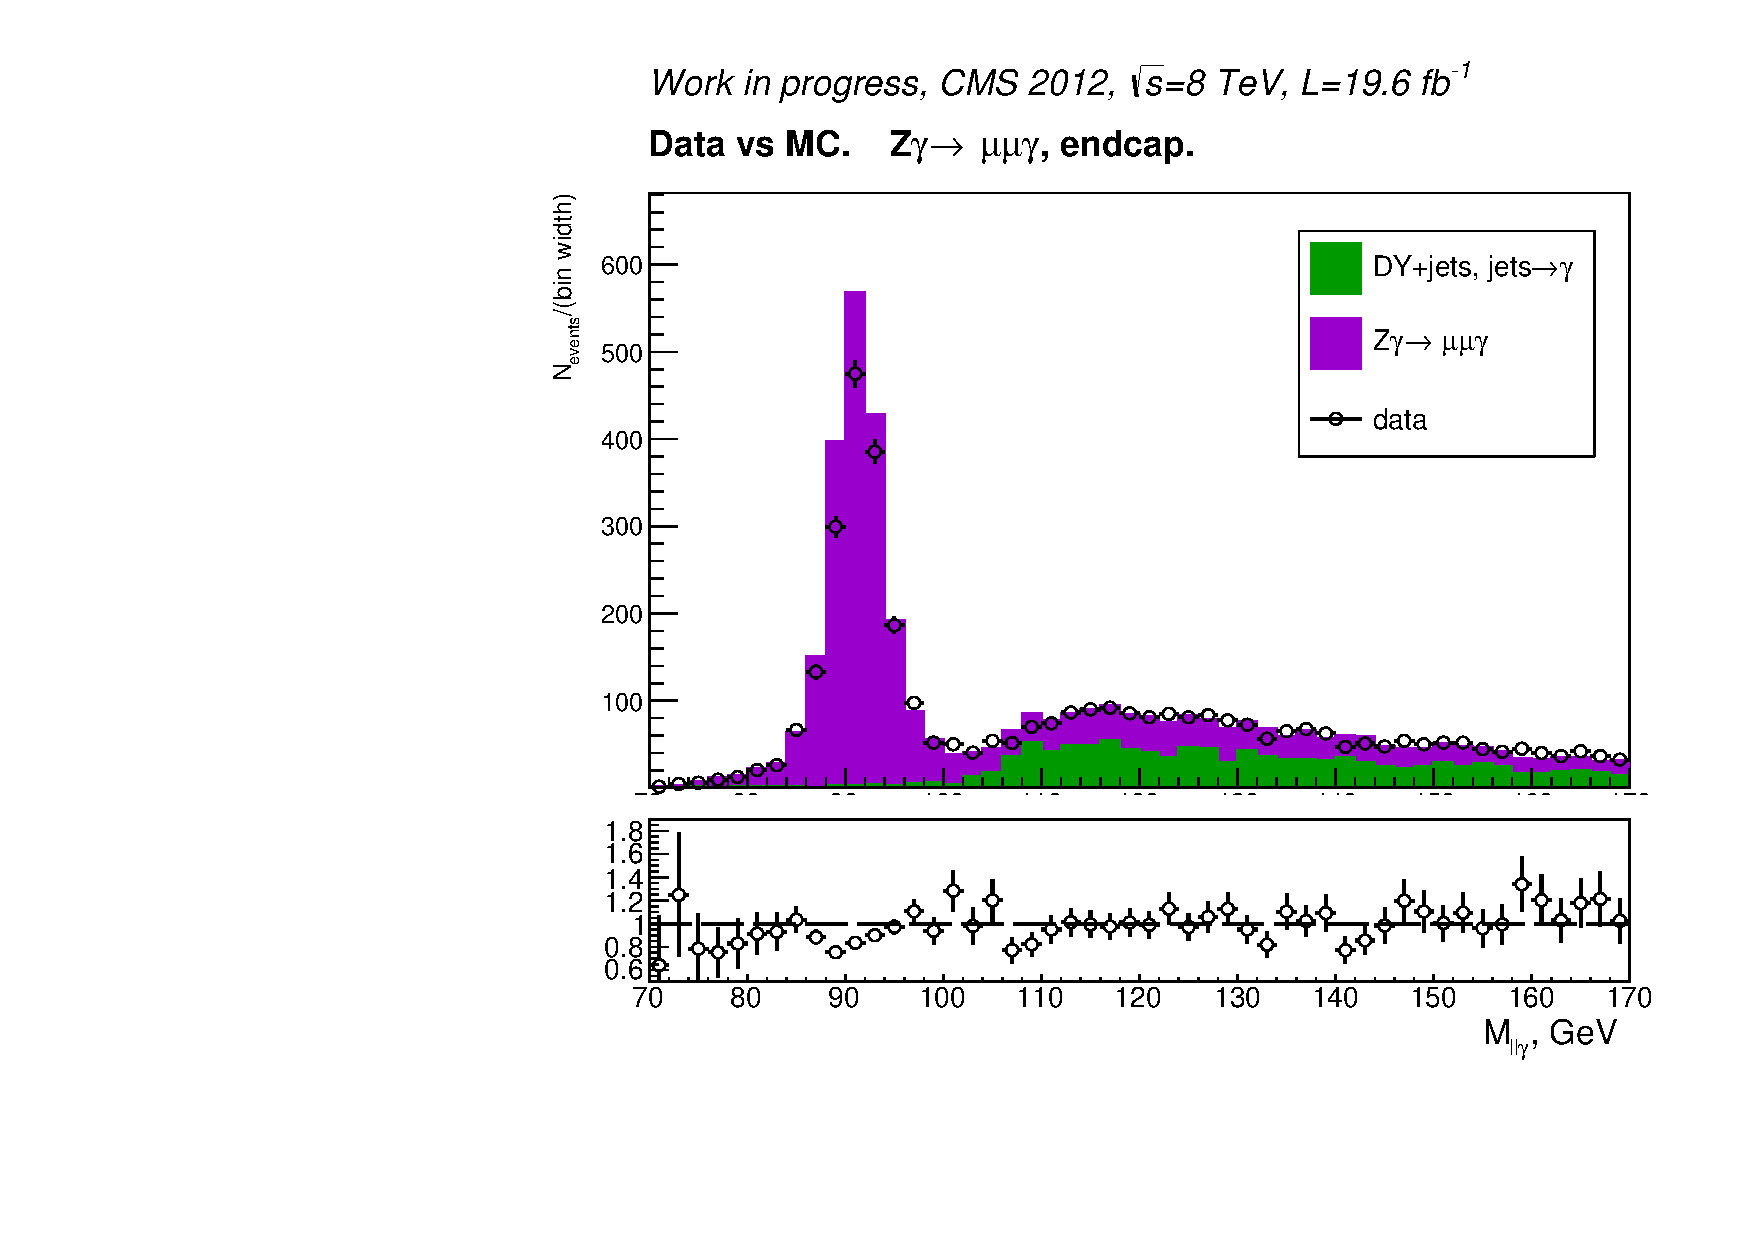
\includegraphics[width=0.45\textwidth]{../figs/figs_v11/MUON_ZGamma/PrepareYields/c_TotalDATAvsMC_Endcap__MpholeplepVERY_PRELIMINARY.pdf}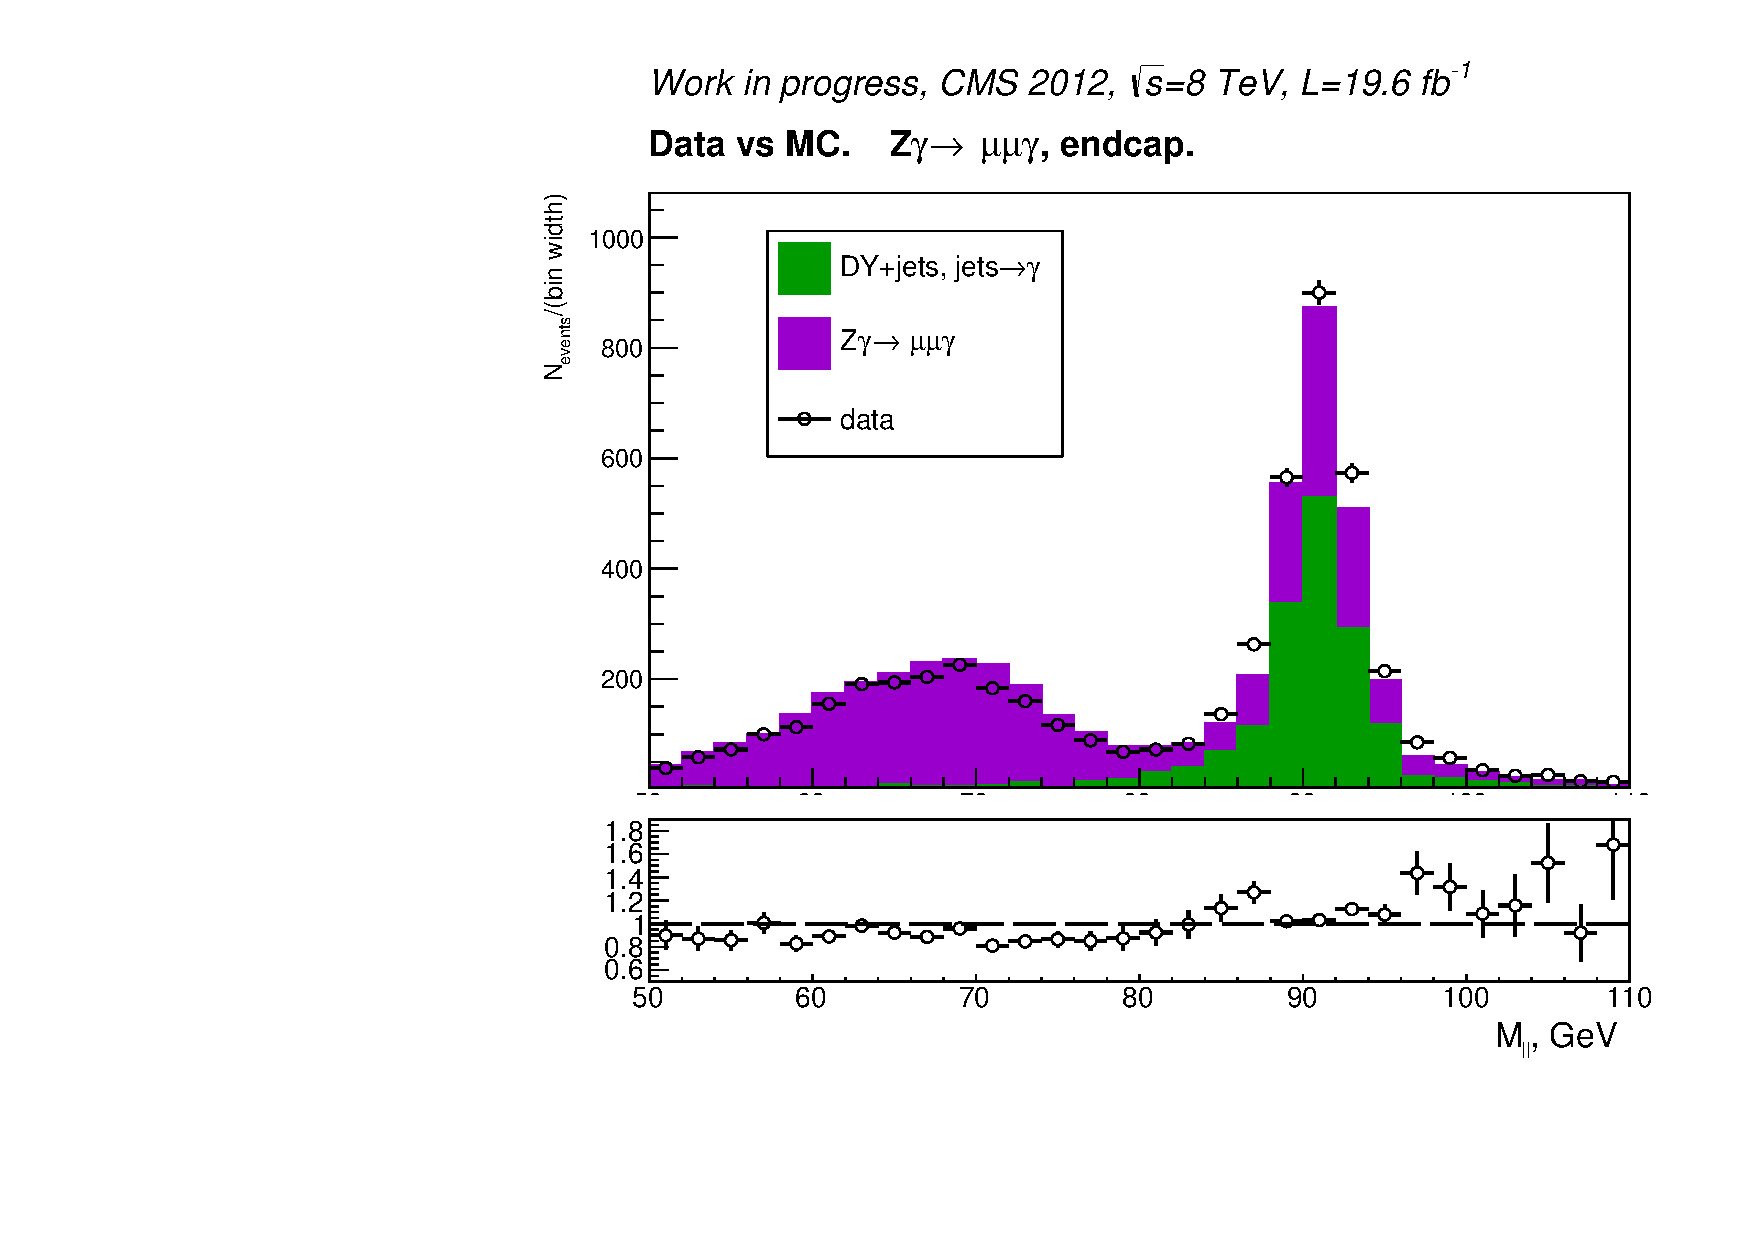
\includegraphics[width=0.45\textwidth]{../figs/figs_v11/MUON_ZGamma/PrepareYields/c_TotalDATAvsMC_Endcap__MleplepVERY_PRELIMINARY.pdf}\\
  \caption{Distributions of $M_{\mu\mu\gamma}$ (left) and $M_{\mu\mu}$ (right) in $Z\gamma\rightarrow\mu\mu\gamma$-selected events, data vs MC. $P_T^{\gamma}: $15-500~GeV. Left: $M_{\mu\mu\gamma}$, right: $M_{\mu\mu}$. Top: barrel photons, bottom: endcap photons. Peak highly dominated by $Z\gamma$ events corresponds to FSR. }
  \label{fig:Zg_Mleplep_and_Mpholeplep}
  \end{center}
\end{figure}

\begin{figure}[htb]
  \begin{center}
   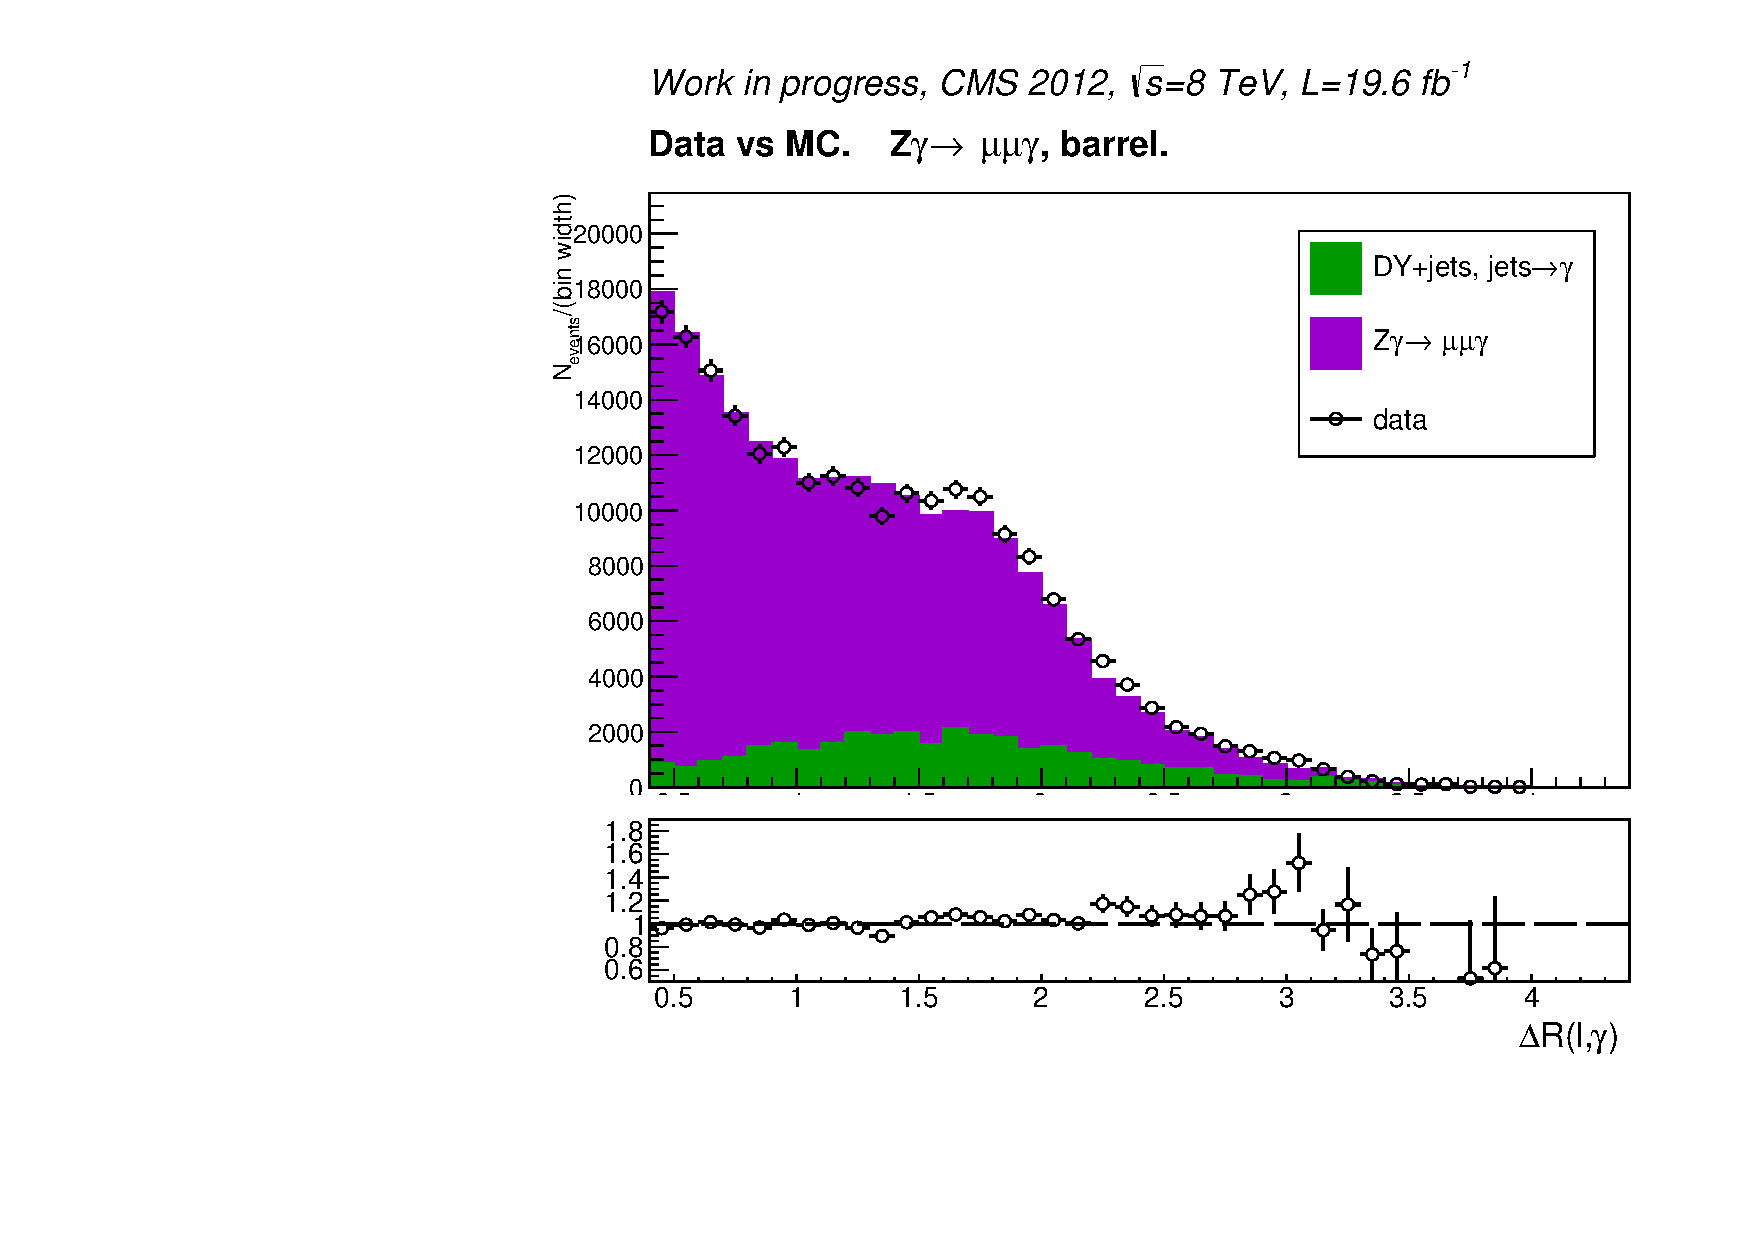
\includegraphics[width=0.45\textwidth]{../figs/figs_v11/MUON_ZGamma/PrepareYields/c_TotalDATAvsMC_Barrel__lep1PhoDeltaRVERY_PRELIMINARY.pdf}   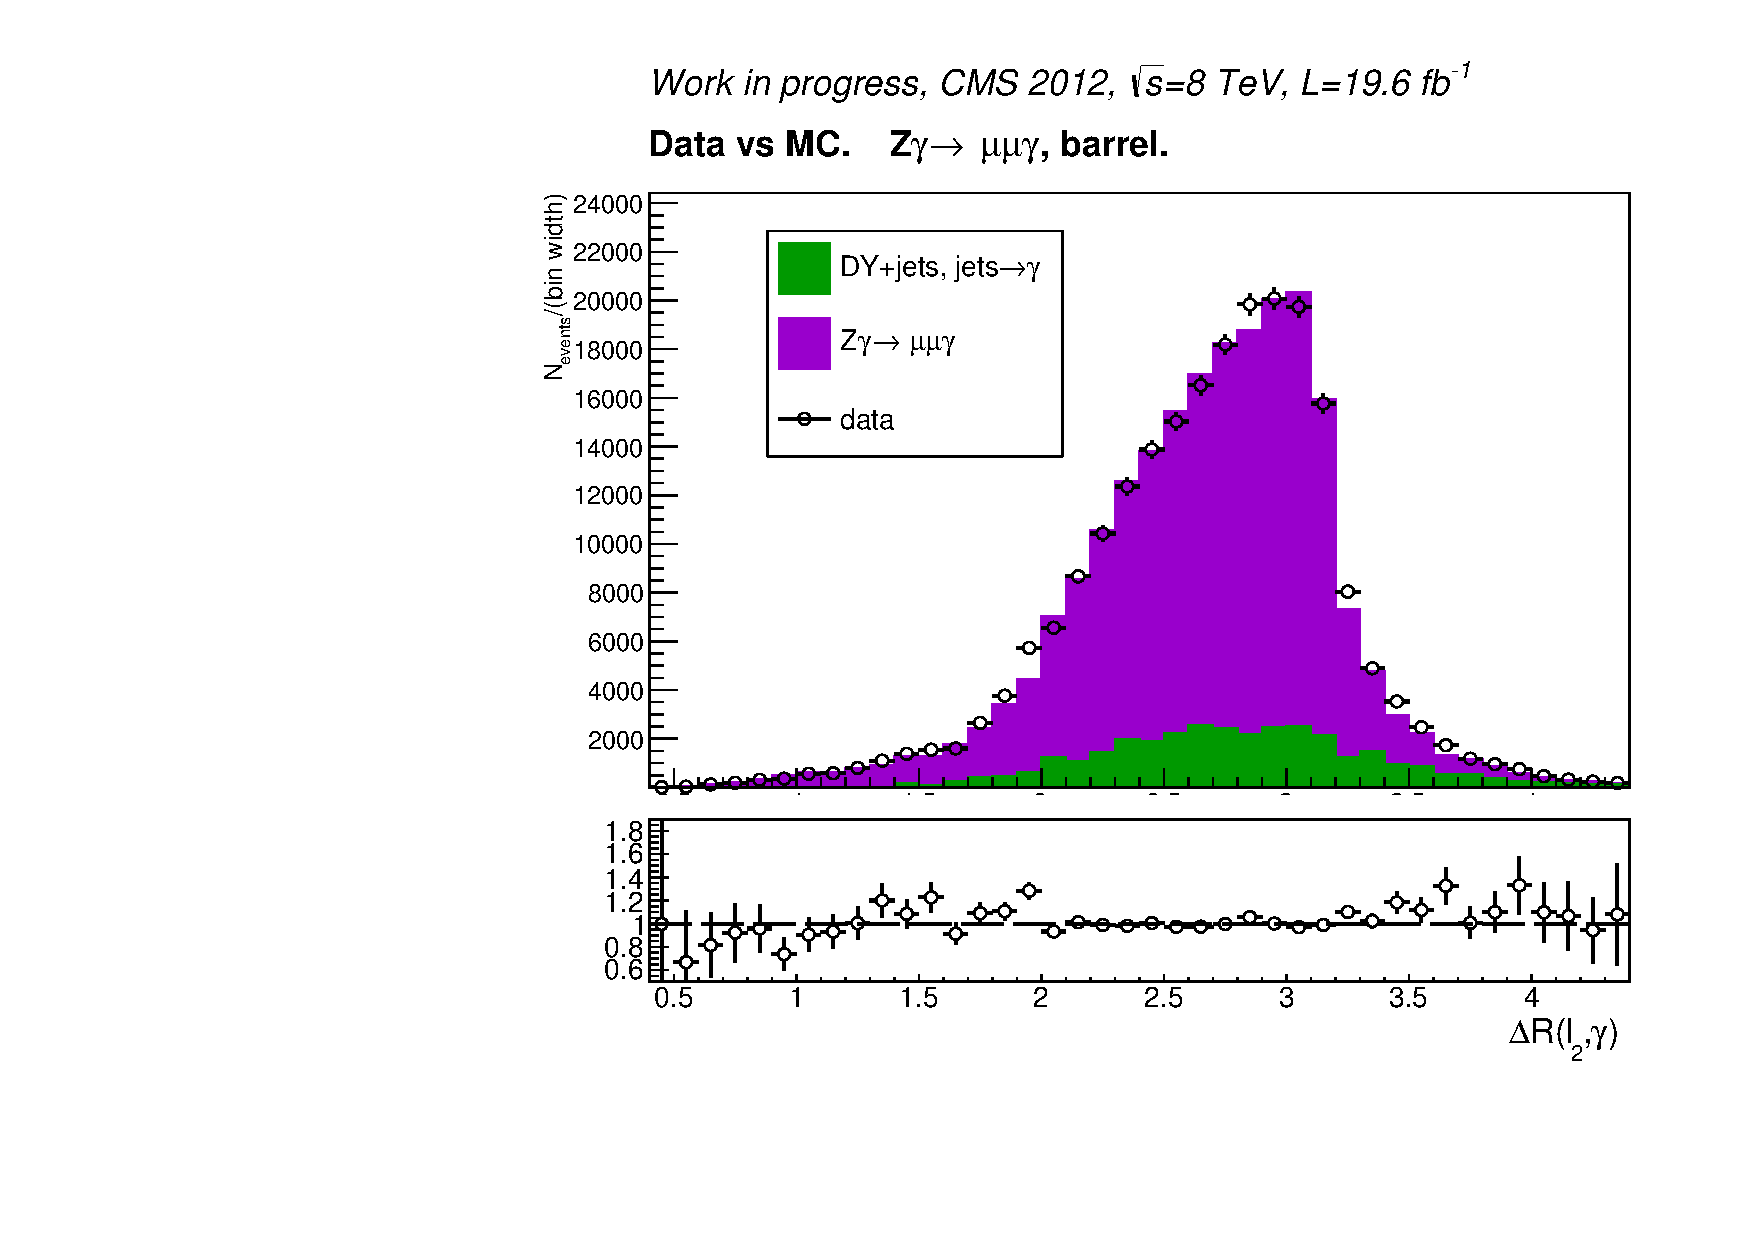
\includegraphics[width=0.45\textwidth]{../figs/figs_v11/MUON_ZGamma/PrepareYields/c_TotalDATAvsMC_Barrel__lep2PhoDeltaRVERY_PRELIMINARY.pdf}\\
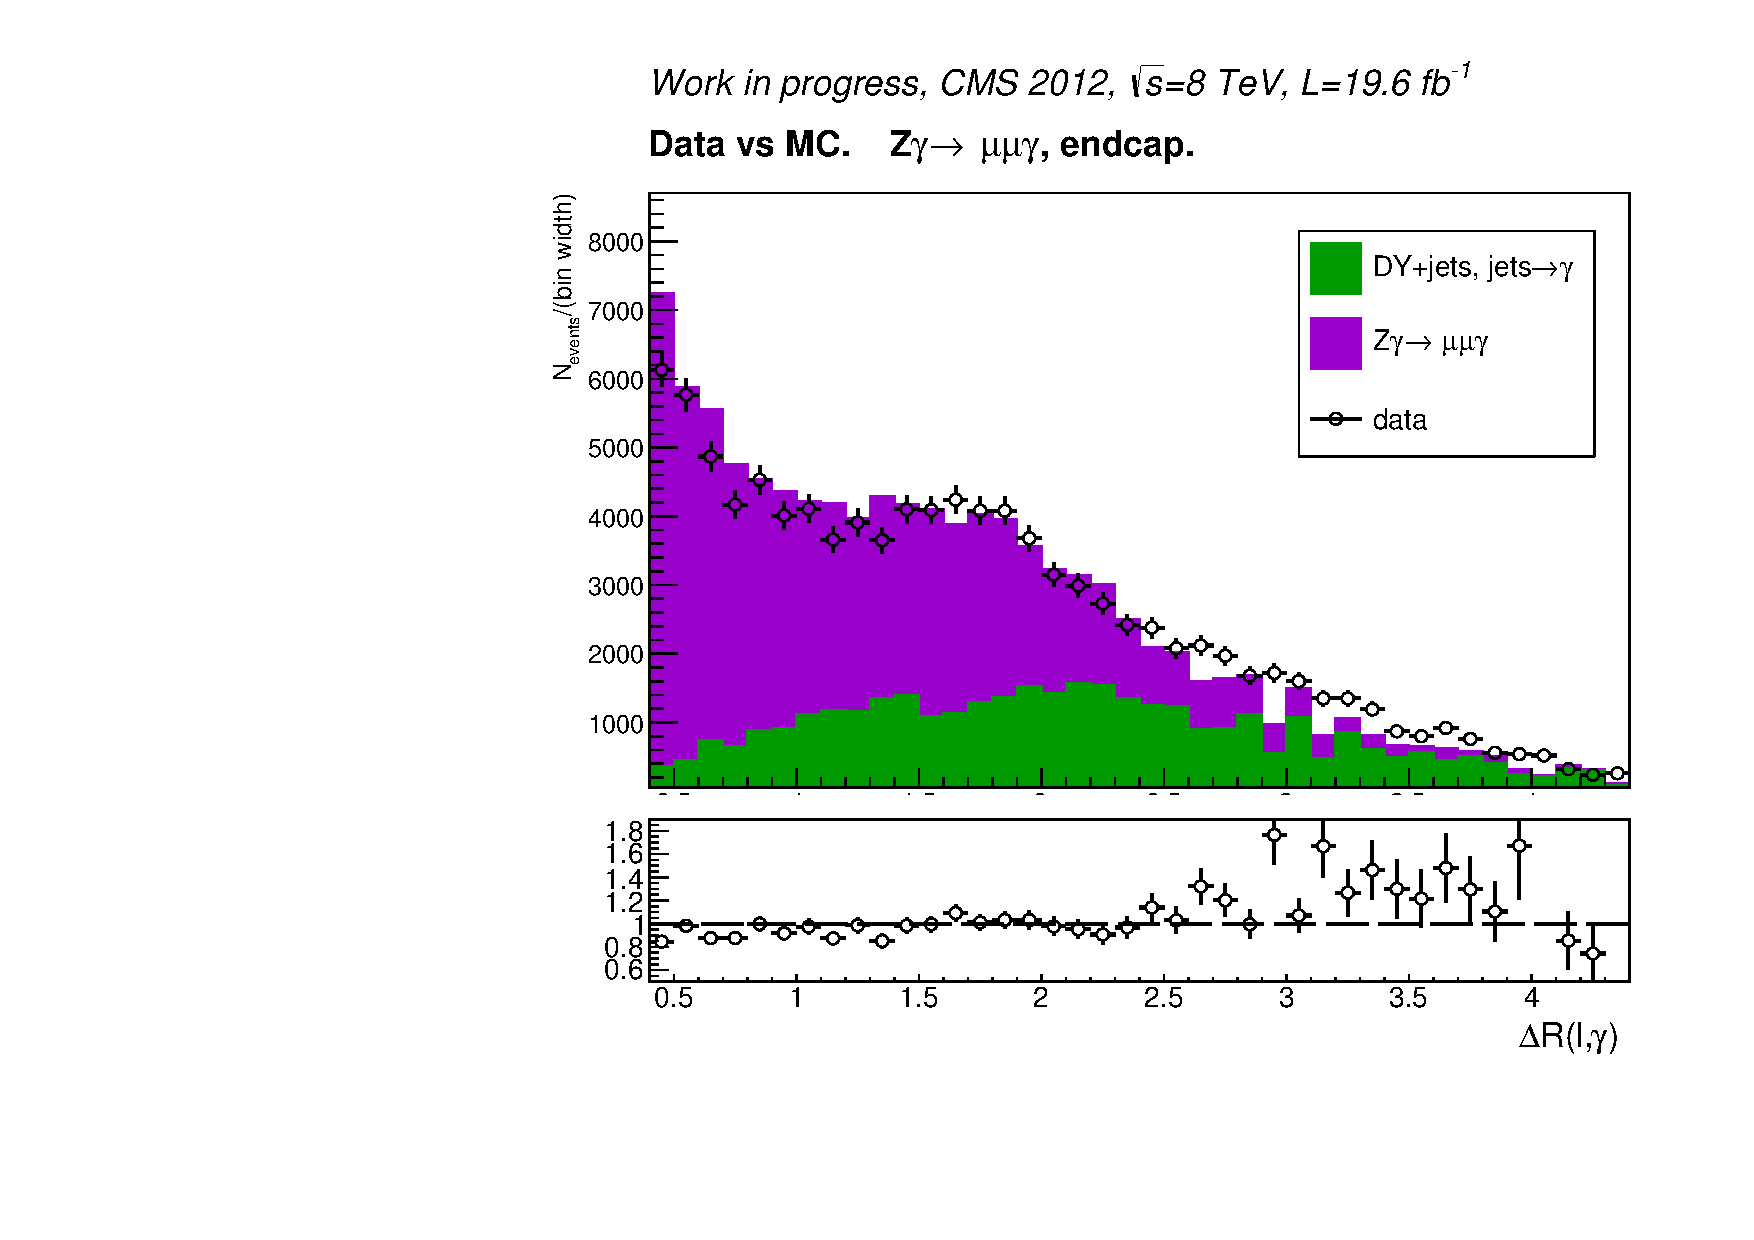
\includegraphics[width=0.45\textwidth]{../figs/figs_v11/MUON_ZGamma/PrepareYields/c_TotalDATAvsMC_Endcap__lep1PhoDeltaRVERY_PRELIMINARY.pdf}   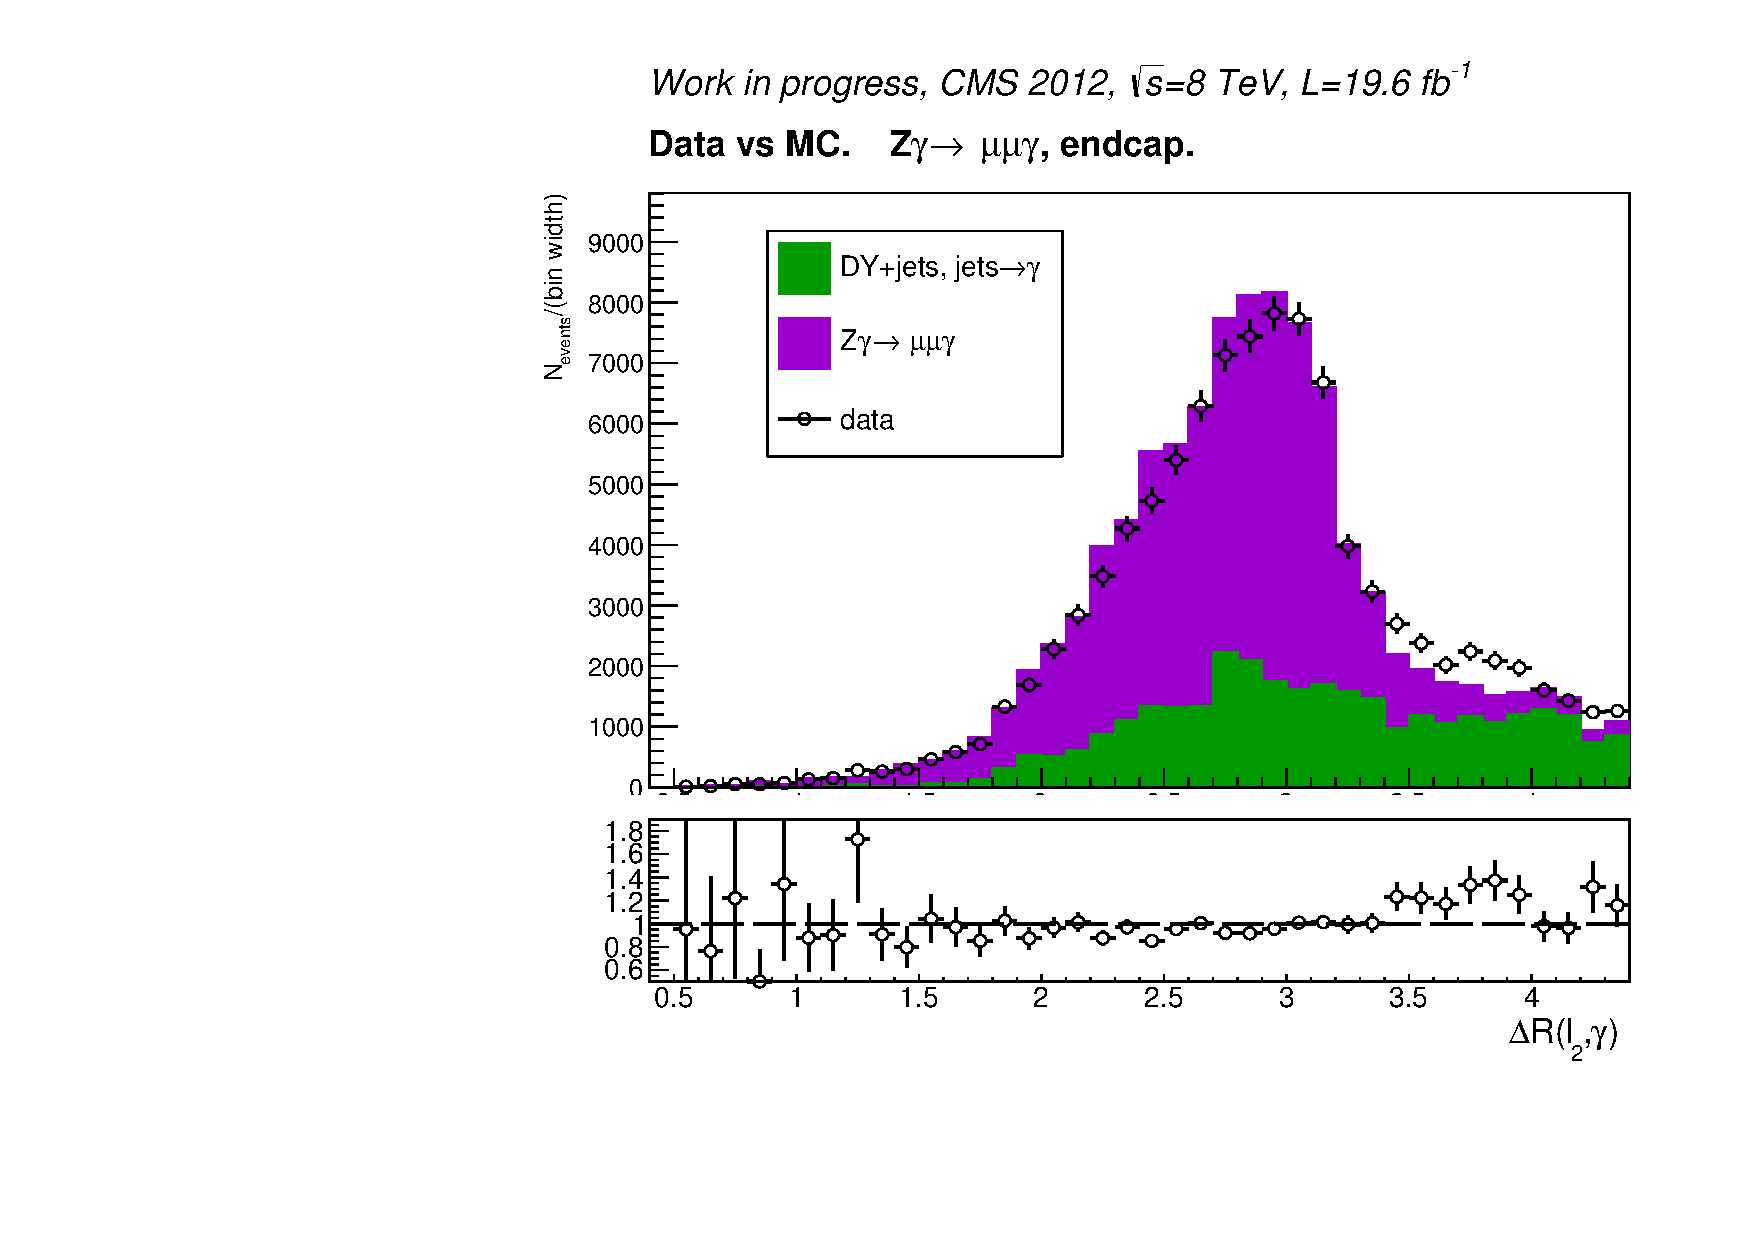
\includegraphics[width=0.45\textwidth]{../figs/figs_v11/MUON_ZGamma/PrepareYields/c_TotalDATAvsMC_Endcap__lep2PhoDeltaRVERY_PRELIMINARY.pdf}    \\
  \caption{Distributions of $\Delta R(\mu_1,\gamma)$ (left) and $\Delta R(\mu_2,\gamma)$ (right) in $Z\gamma\rightarrow\mu\mu\gamma$-selected events, data vs MC. $P_T^{\gamma}: $15-500~GeV. Left: $M_{\mu\mu\gamma}$, right: $M_{\mu\mu}$. Top: barrel photons, bottom: endcap. Peak highly dominated by $Z\gamma$ events corresponds to FSR.}
  \label{fig:Zg_ISRandFSR_dR}
  \end{center}
\end{figure}

\begin{figure}[htb]
  \begin{center}
   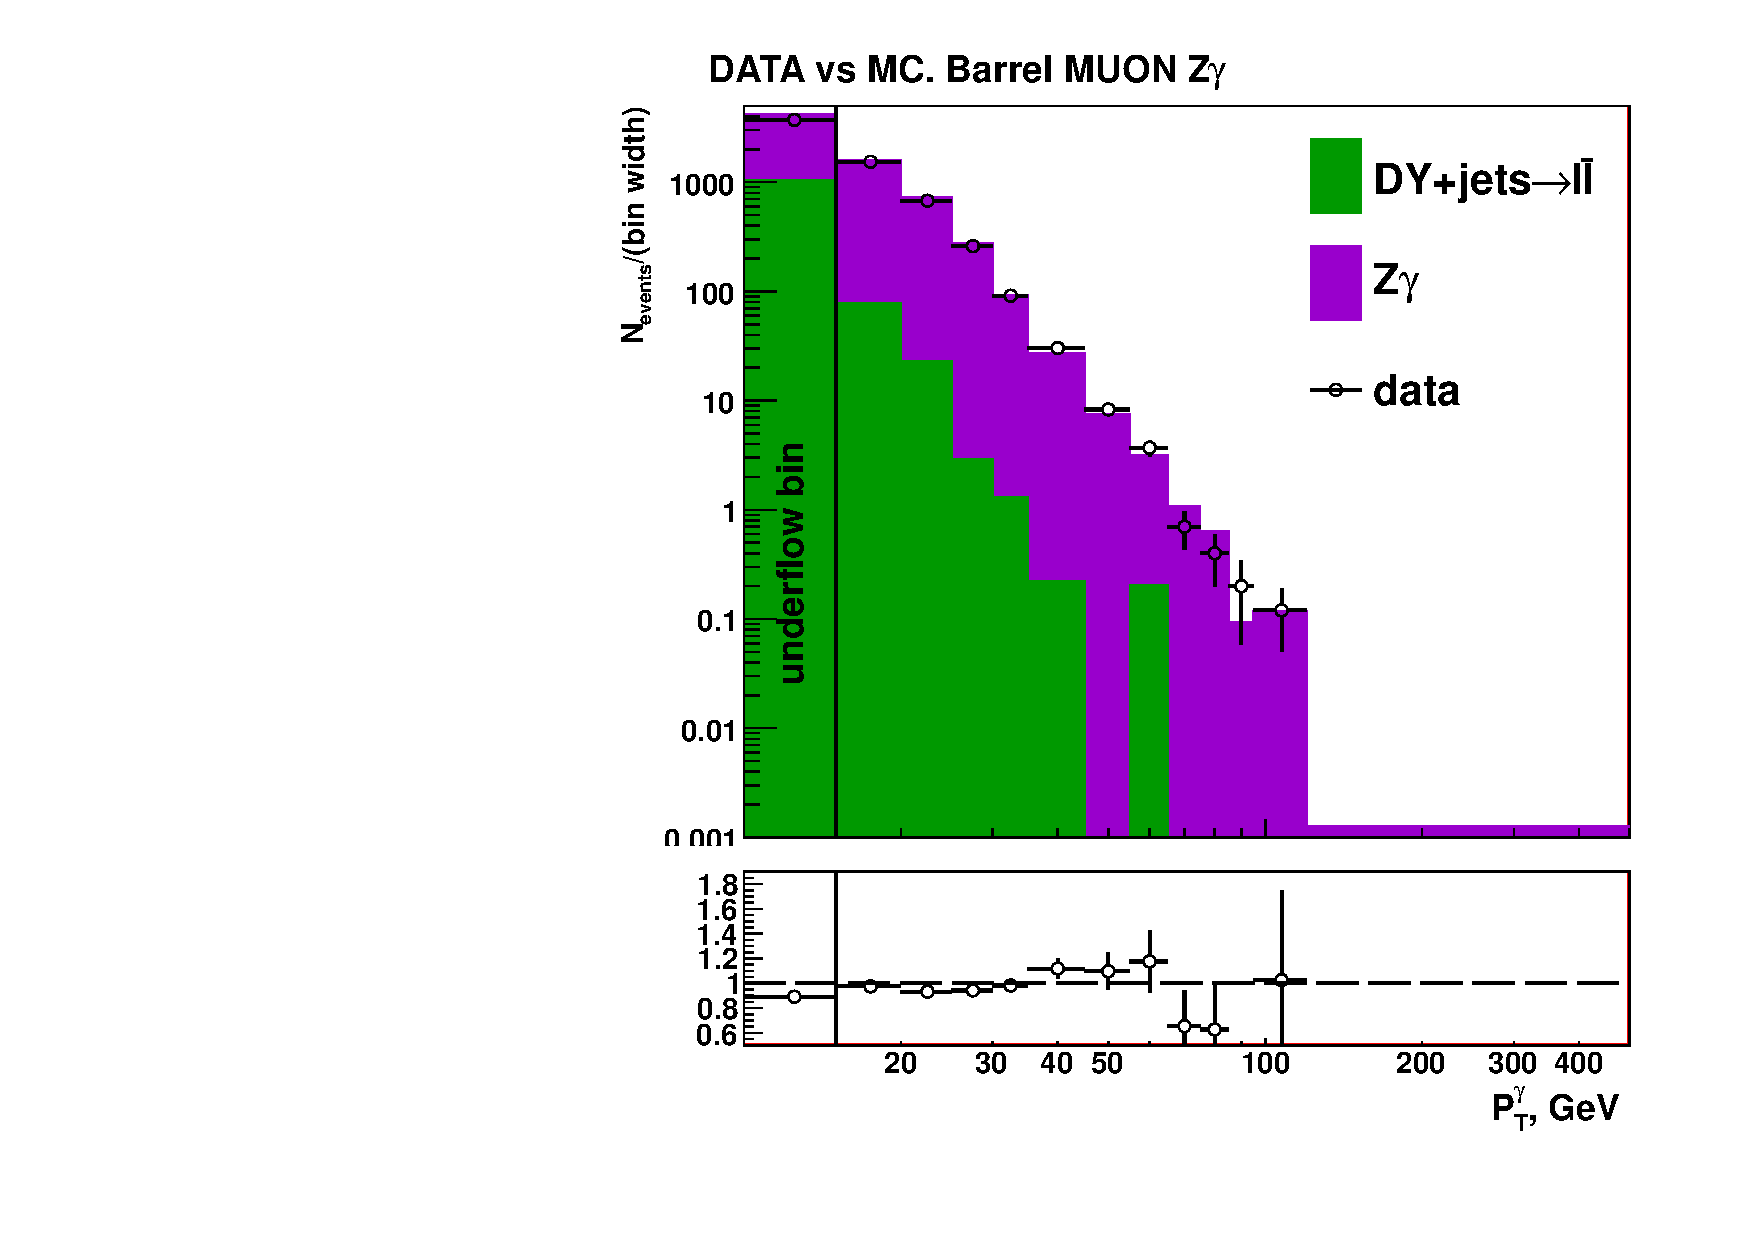
\includegraphics[width=0.45\textwidth]{../figs/figs_v11/MUON_ZGamma/PrepareYields/c_TotalDATAvsMC_Barrel__phoEtFSR.pdf}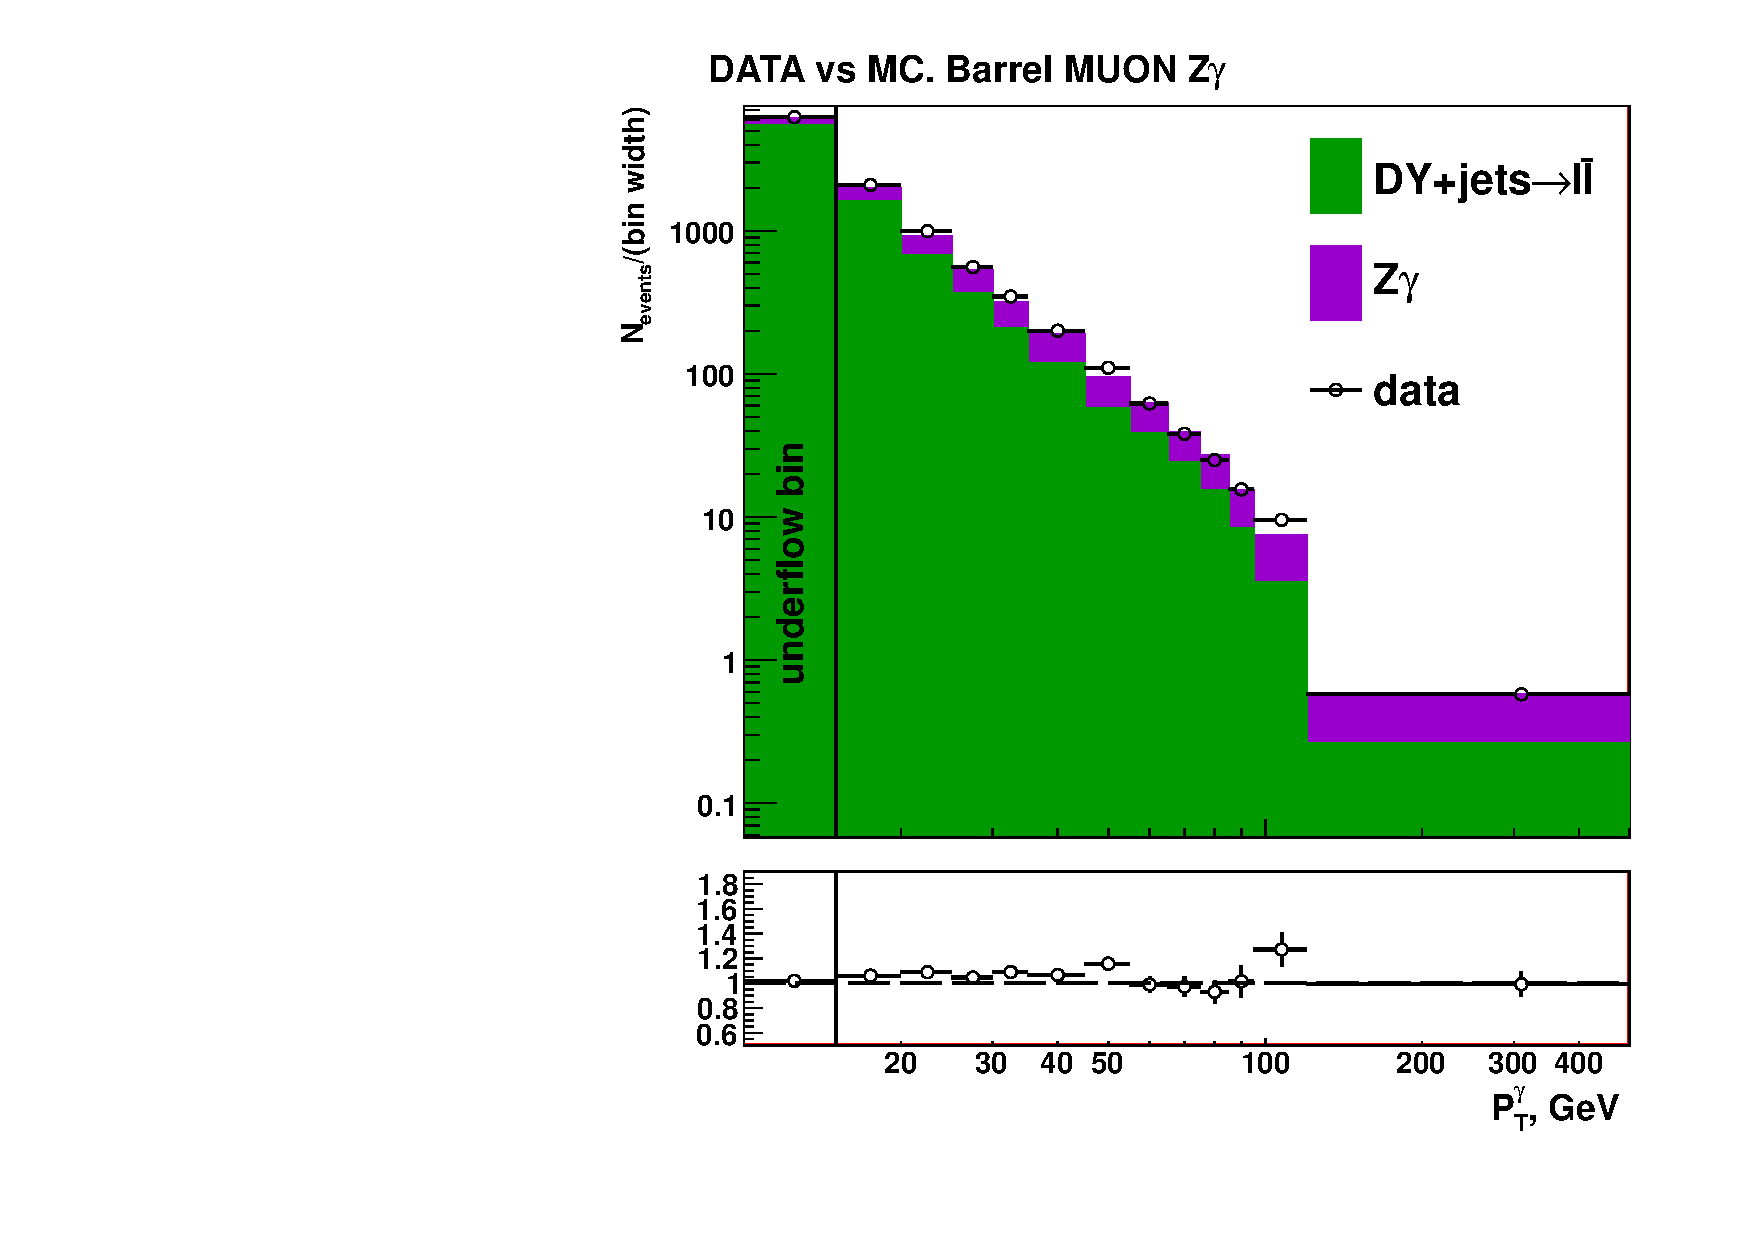
\includegraphics[width=0.45\textwidth]{../figs/figs_v11/MUON_ZGamma/PrepareYields/c_TotalDATAvsMC_Barrel__phoEtFSR_EXCLUDED.pdf}\\
   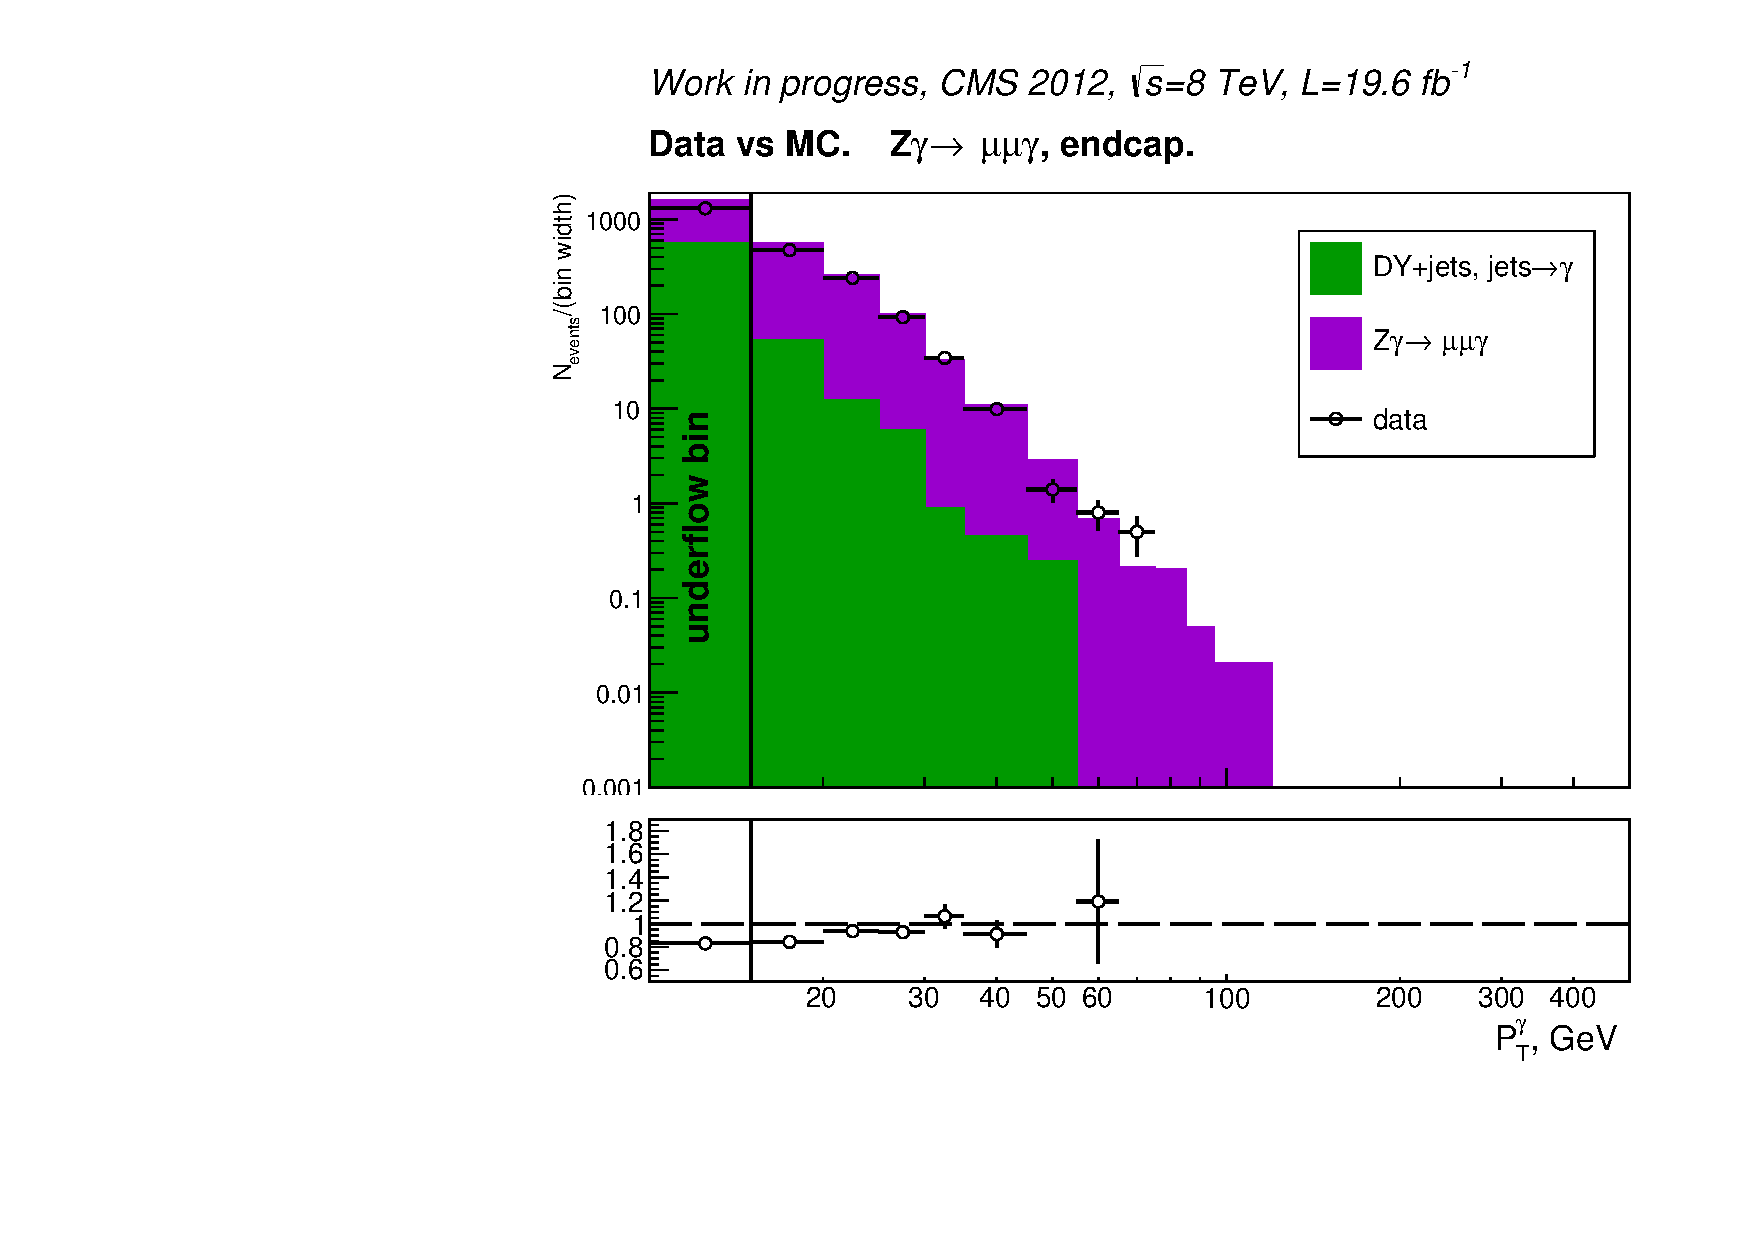
\includegraphics[width=0.45\textwidth]{../figs/figs_v11/MUON_ZGamma/PrepareYields/c_TotalDATAvsMC_Endcap__phoEtFSR.pdf}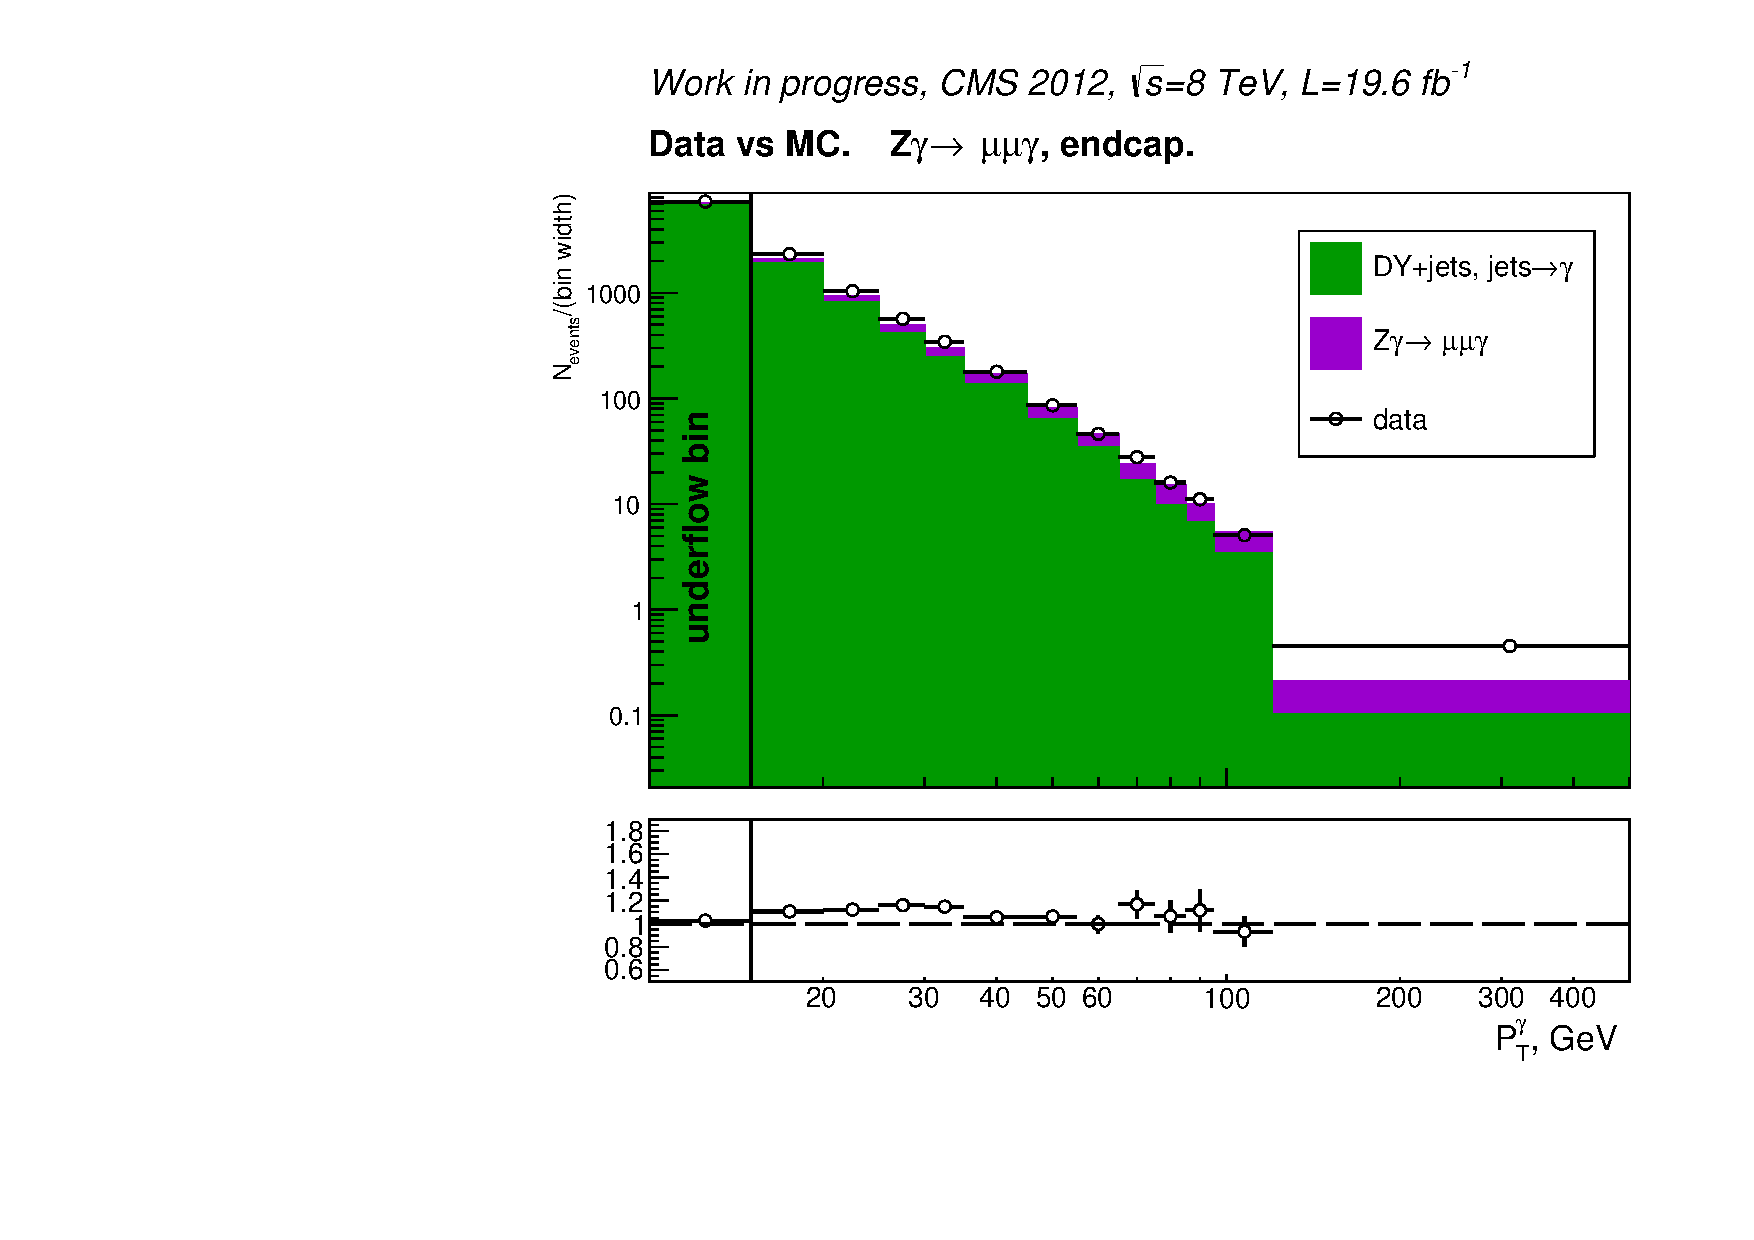
\includegraphics[width=0.45\textwidth]{../figs/figs_v11/MUON_ZGamma/PrepareYields/c_TotalDATAvsMC_Endcap__phoEtFSR_EXCLUDED.pdf}\\
  \caption{$Z\gamma$-selected FSR (left) and ISR (right) events, data vs MC.}
  \label{fig:Zg_ISRandFSR_phoEt}
  \end{center}
\end{figure}

\begin{figure}[htb]
  \begin{center}
   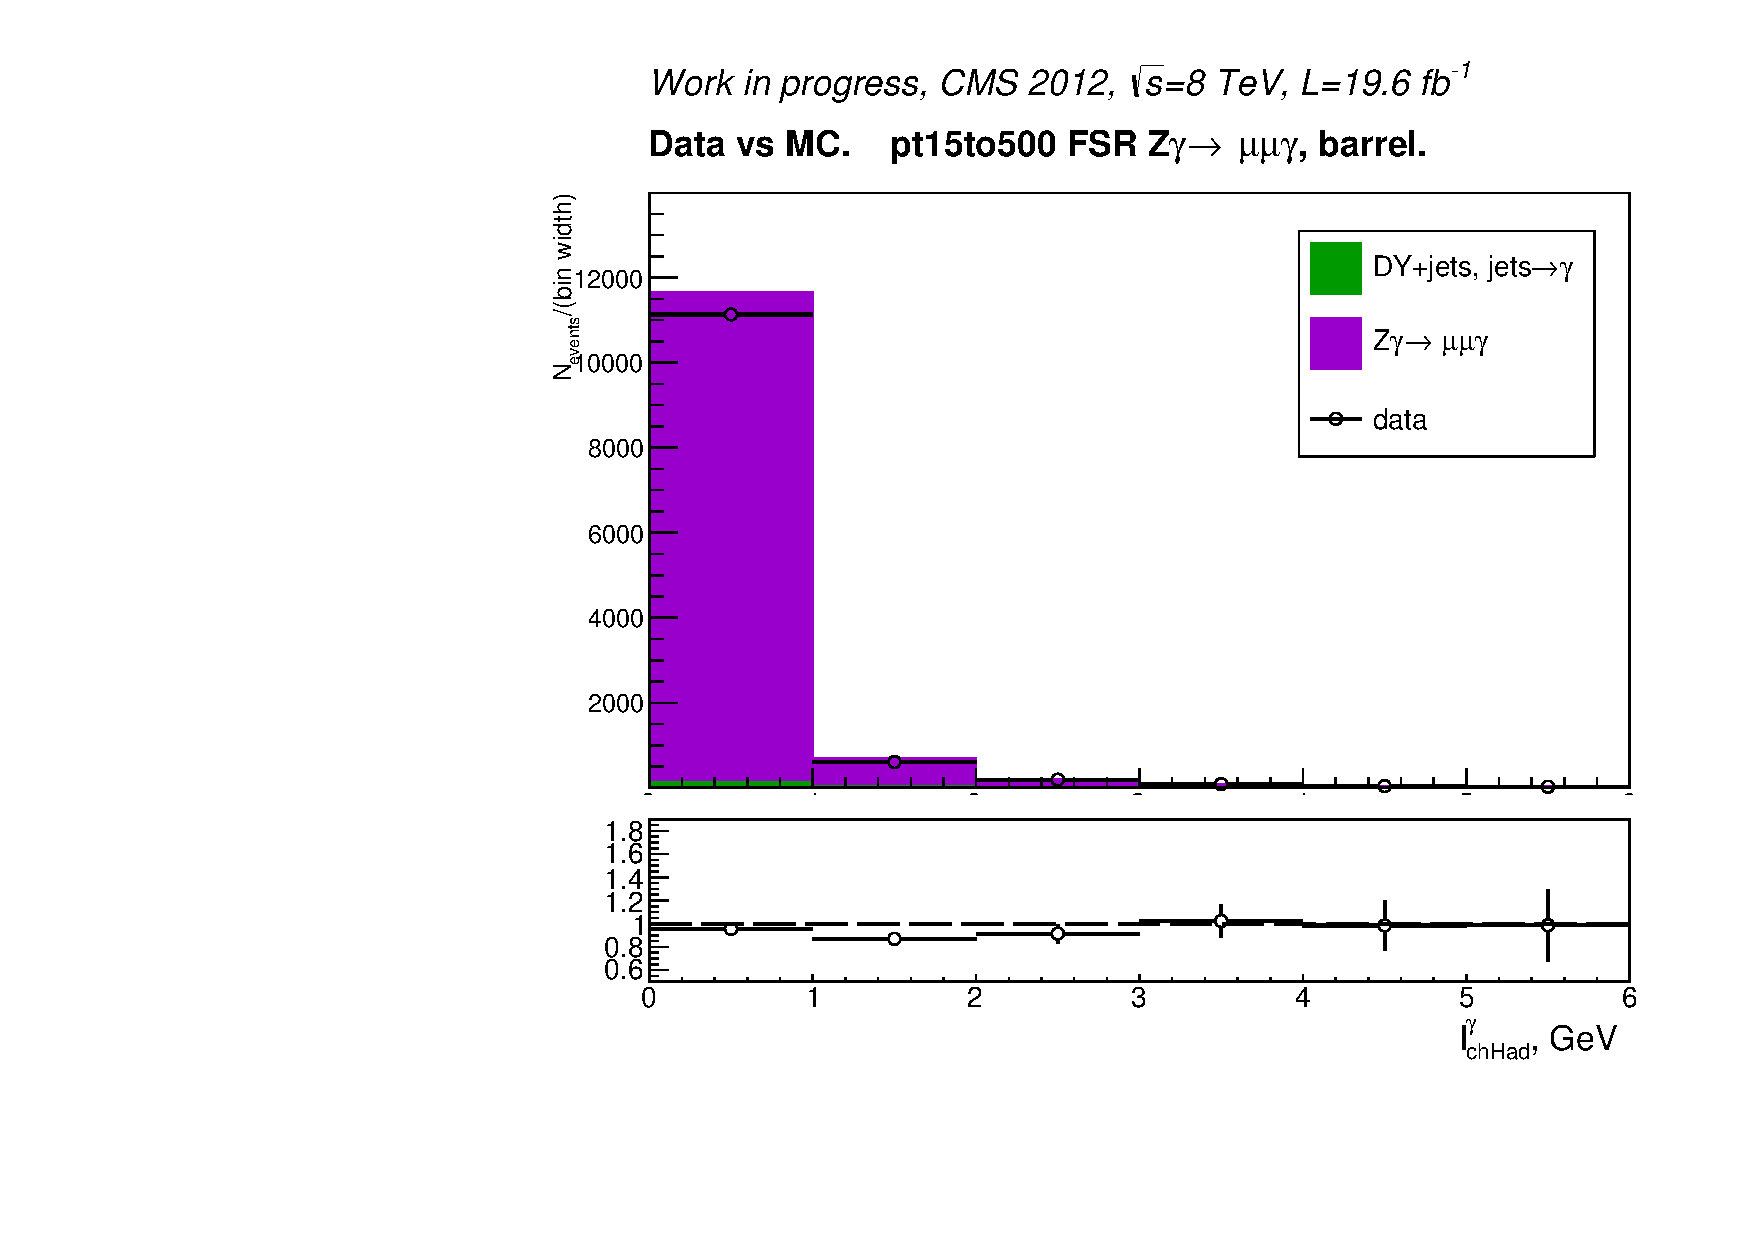
\includegraphics[width=0.45\textwidth]{../figs/figs_v11/MUON_ZGamma/PrepareYields/c_TotalDATAvsMC_Barrel__phoPFChIsoCorrFSR_pt15to500_FSR.pdf}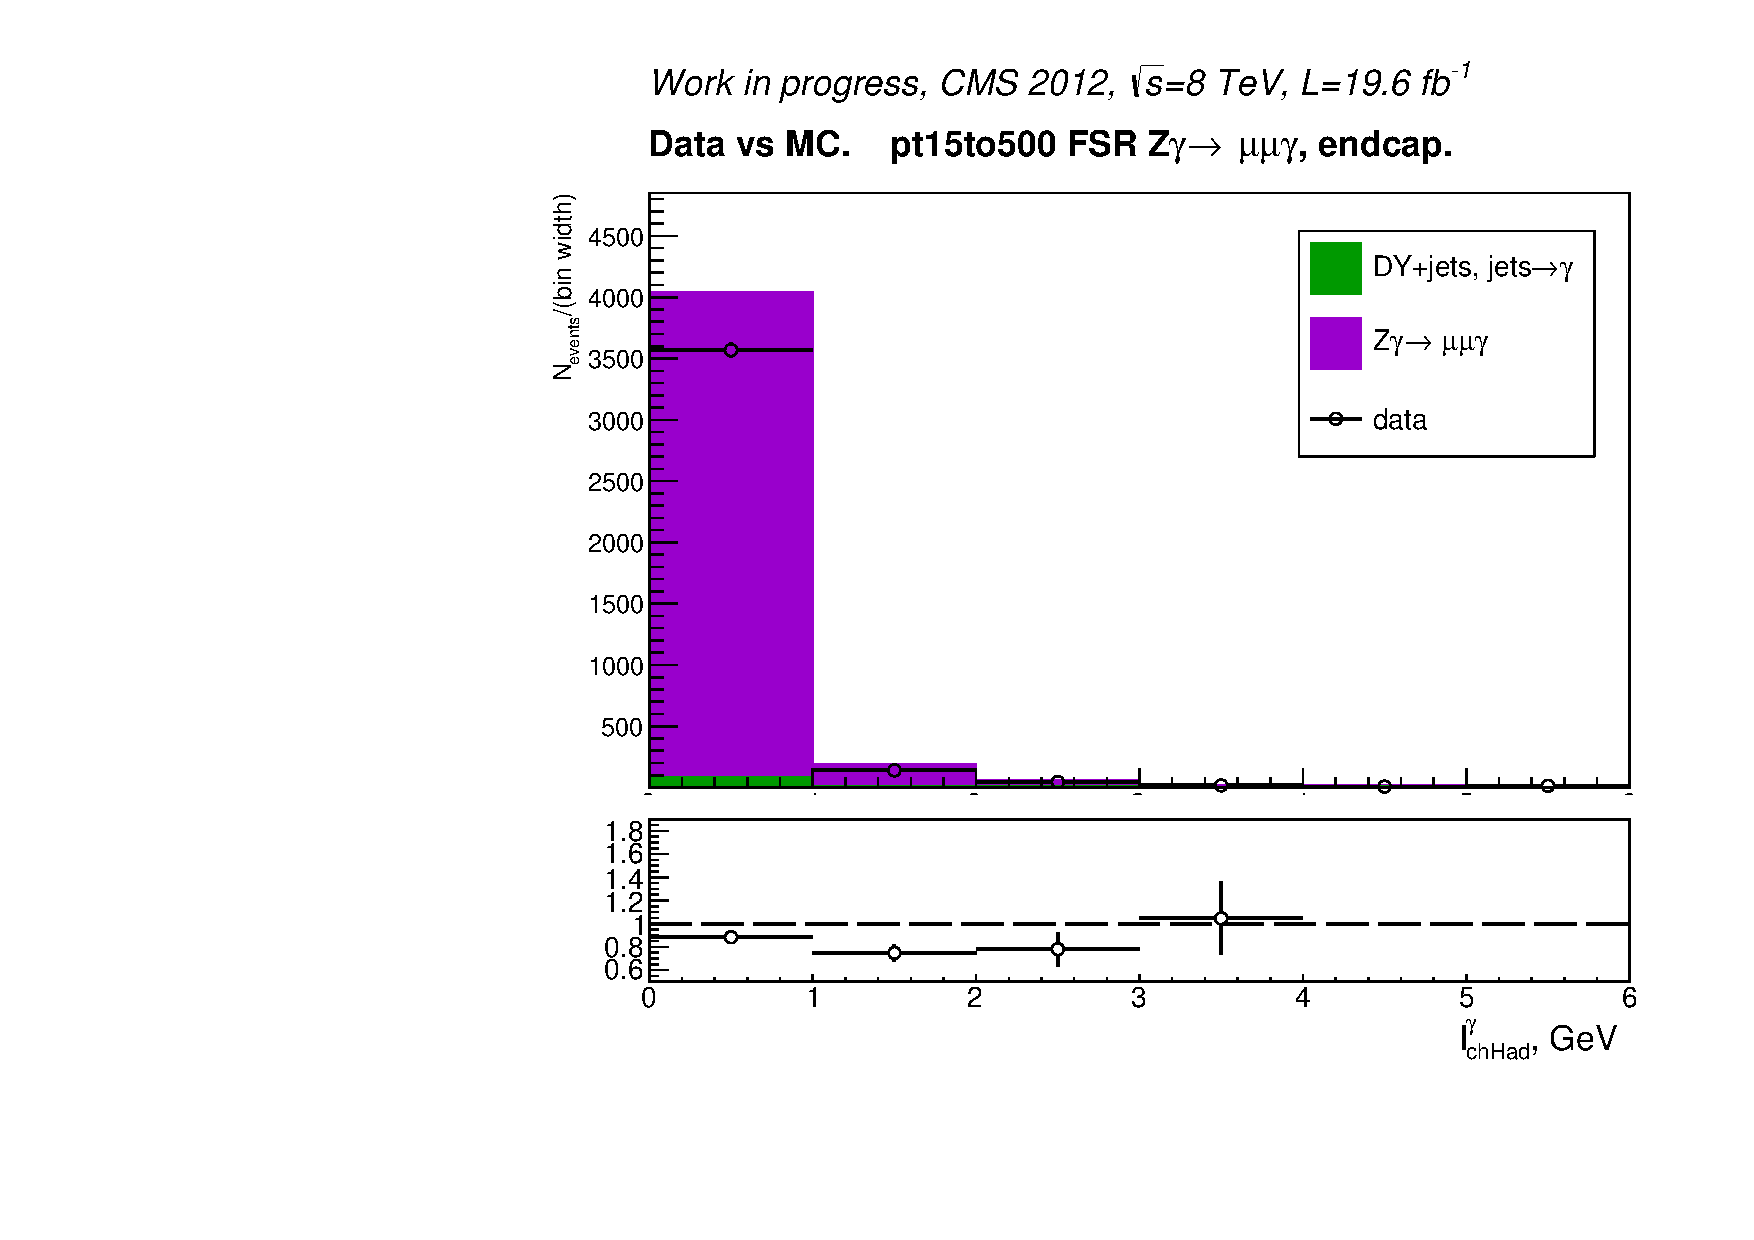
\includegraphics[width=0.45\textwidth]{../figs/figs_v11/MUON_ZGamma/PrepareYields/c_TotalDATAvsMC_Endcap__phoPFChIsoCorrFSR_pt15to500_FSR.pdf}\\
  \caption{$Z\gamma$-selected FSR events, data vs MC. $P_T^{\gamma}>$15~GeV. Distributions of $I_{chHad}^{\gamma}$ used for preparing real-$\gamma$ templates. Fake-$\gamma$ contribution to FSR region is subtracted based on DY+jets MC prediction to prepare real-$\gamma$ templates.}
  \label{fig:Zg_FSR_phoPFChIsoCorr}
  \end{center}
\end{figure}

\begin{figure}[htb]
  \begin{center}
   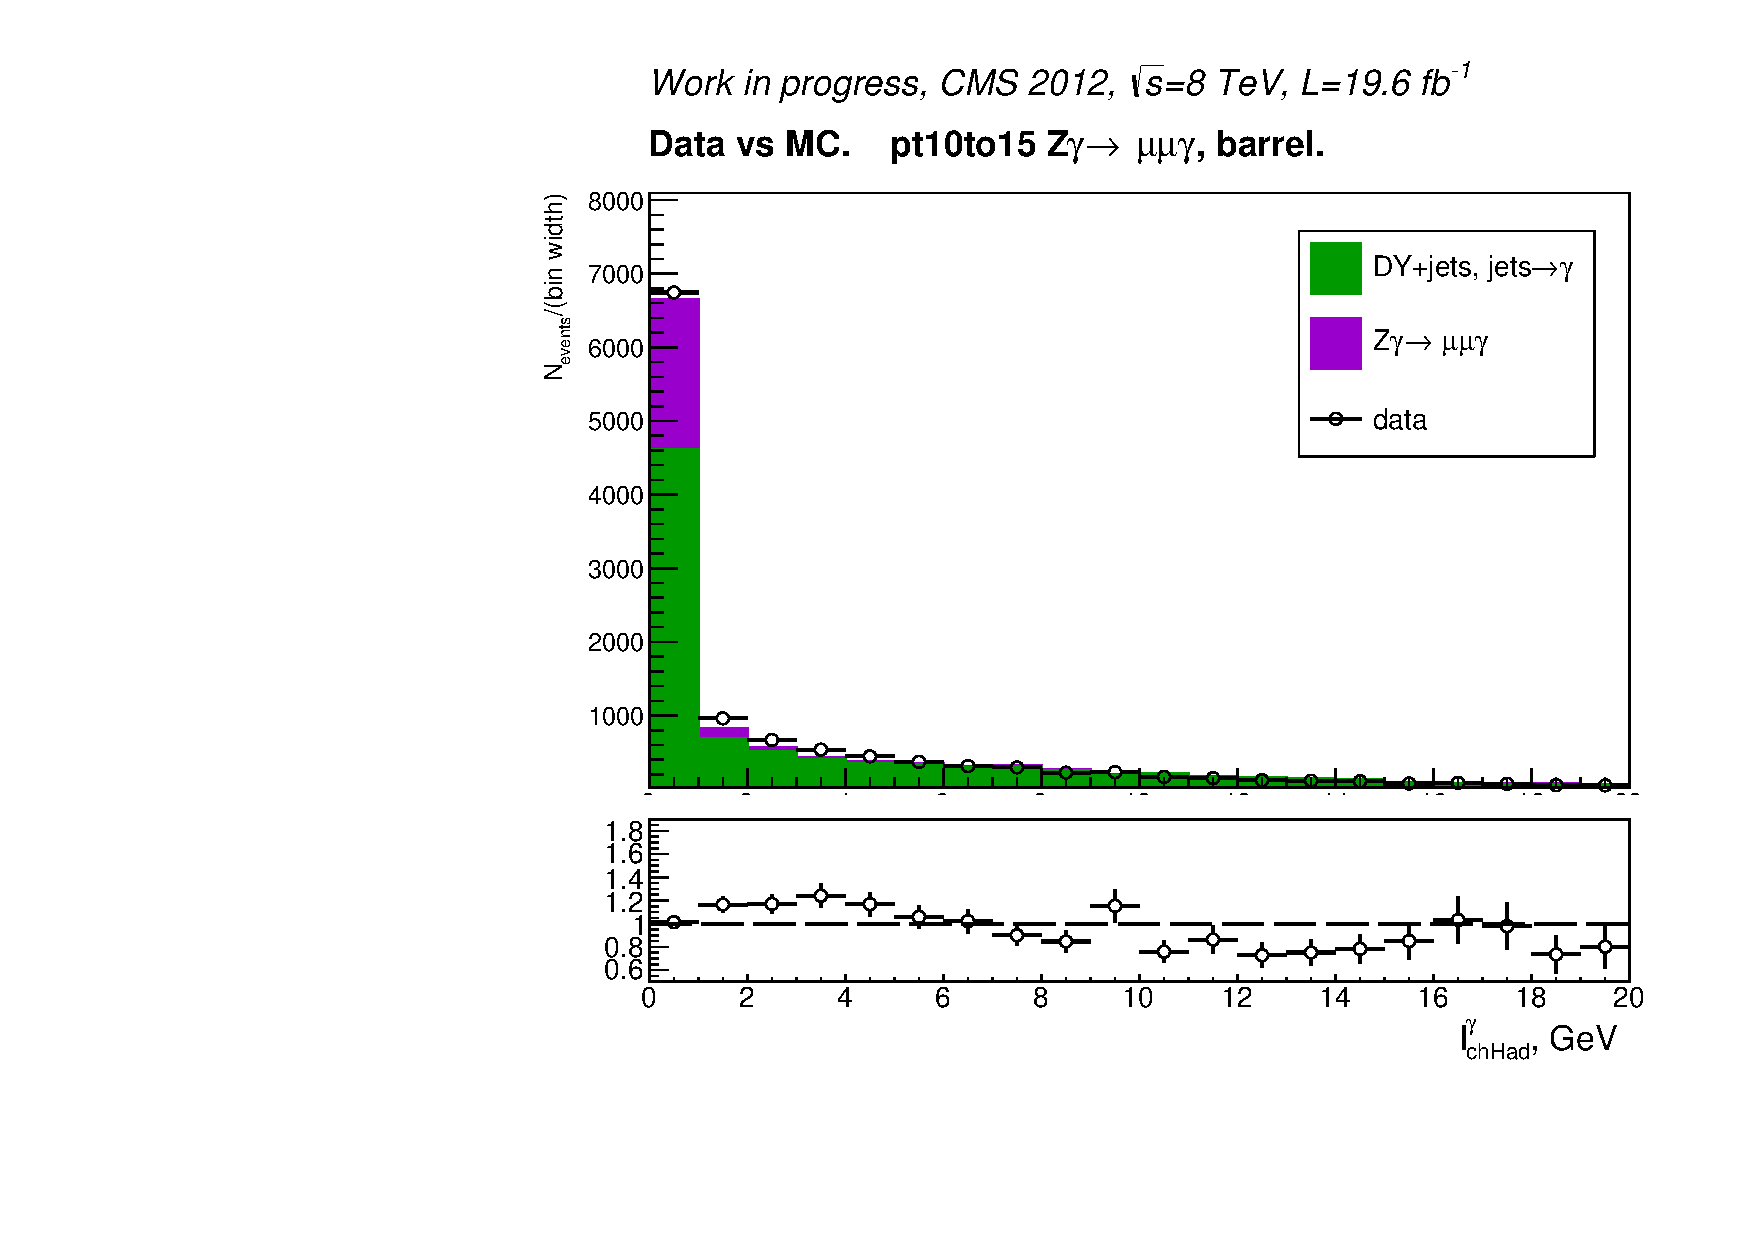
\includegraphics[width=0.45\textwidth]{../figs/figs_v11/MUON_ZGamma/PrepareYields/c_TotalDATAvsMC_Barrel__phoPFChIsoCorrFSR_EXCLUDED_pt10to15_.pdf}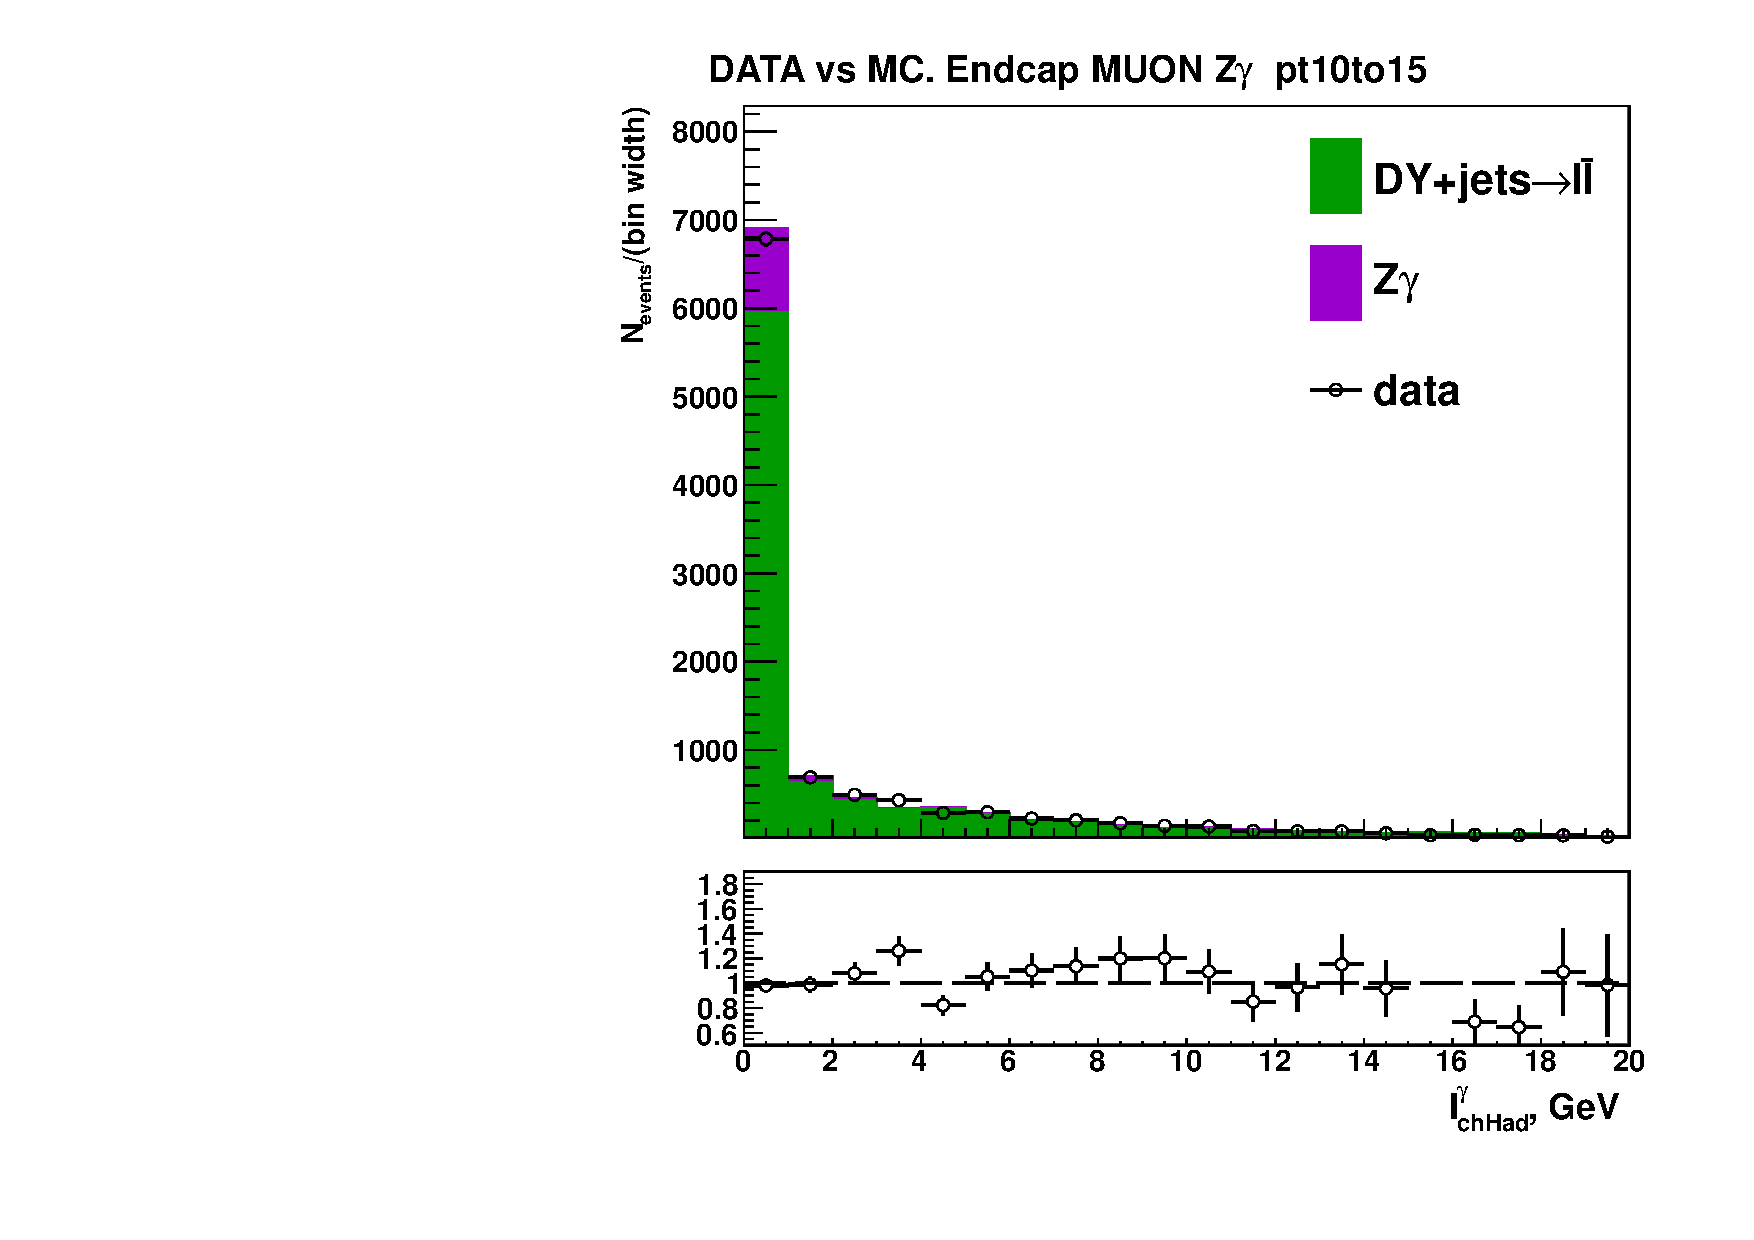
\includegraphics[width=0.45\textwidth]{../figs/figs_v11/MUON_ZGamma/PrepareYields/c_TotalDATAvsMC_Endcap__phoPFChIsoCorrFSR_EXCLUDED_pt10to15_.pdf}\\
  \caption{$Z\gamma$-selected ISR events, data vs MC. 10~GeV$<P_T^{\gamma}<$15~GeV. Distributions of $I_{chHad}^{\gamma}$ used for preparing fake-$\gamma$ templates. Real-$\gamma$ contribution to ISR region is subtracted based on $Z\gamma$ signal MC prediction to prepare fake-$\gamma$ templates.}
  \label{fig:Zg_ISR_phoPFChIsoCorr_pt10to15}
  \end{center}
\end{figure}

\begin{figure}[htb]
  \begin{center}
   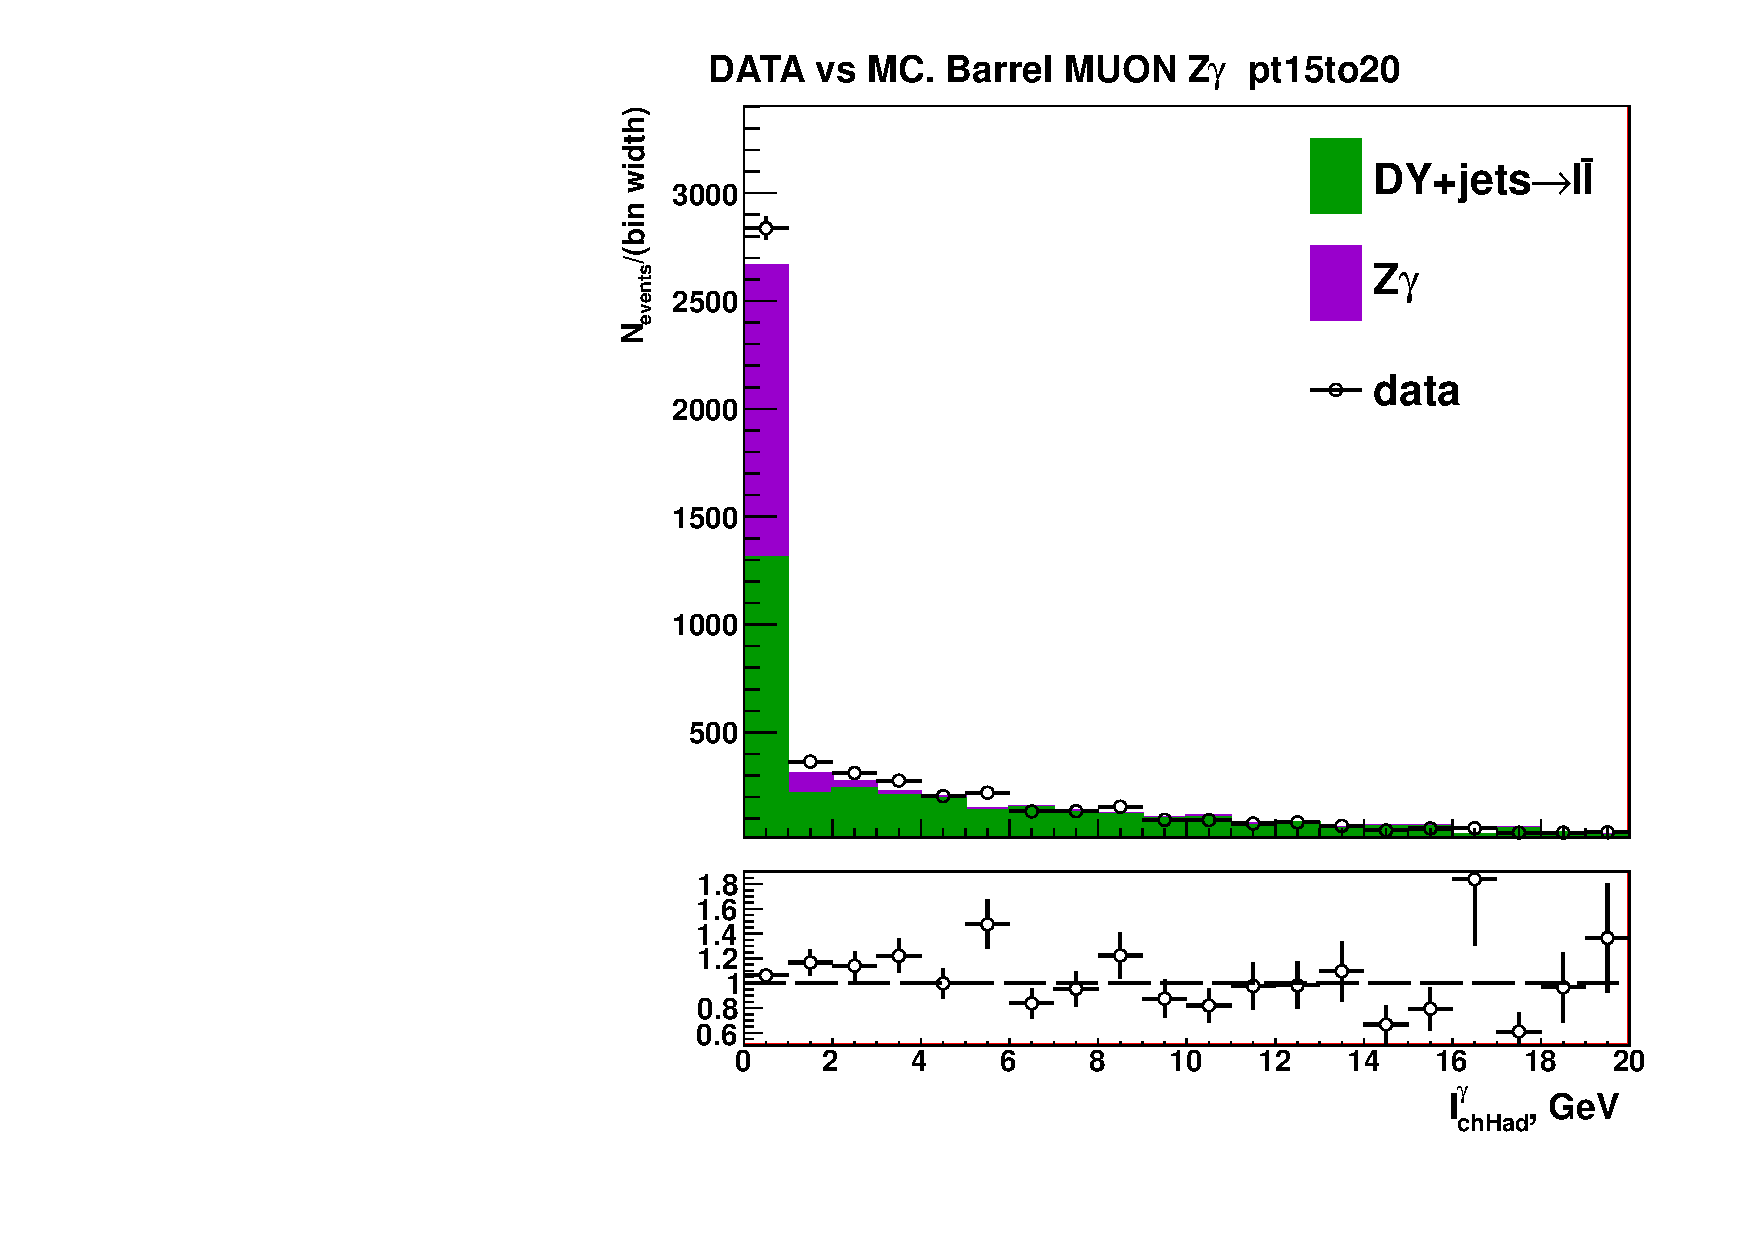
\includegraphics[width=0.32\textwidth]{../figs/figs_v11/MUON_ZGamma/PrepareYields/c_TotalDATAvsMC_Barrel__phoPFChIsoCorrFSR_EXCLUDED_pt15to20_.pdf}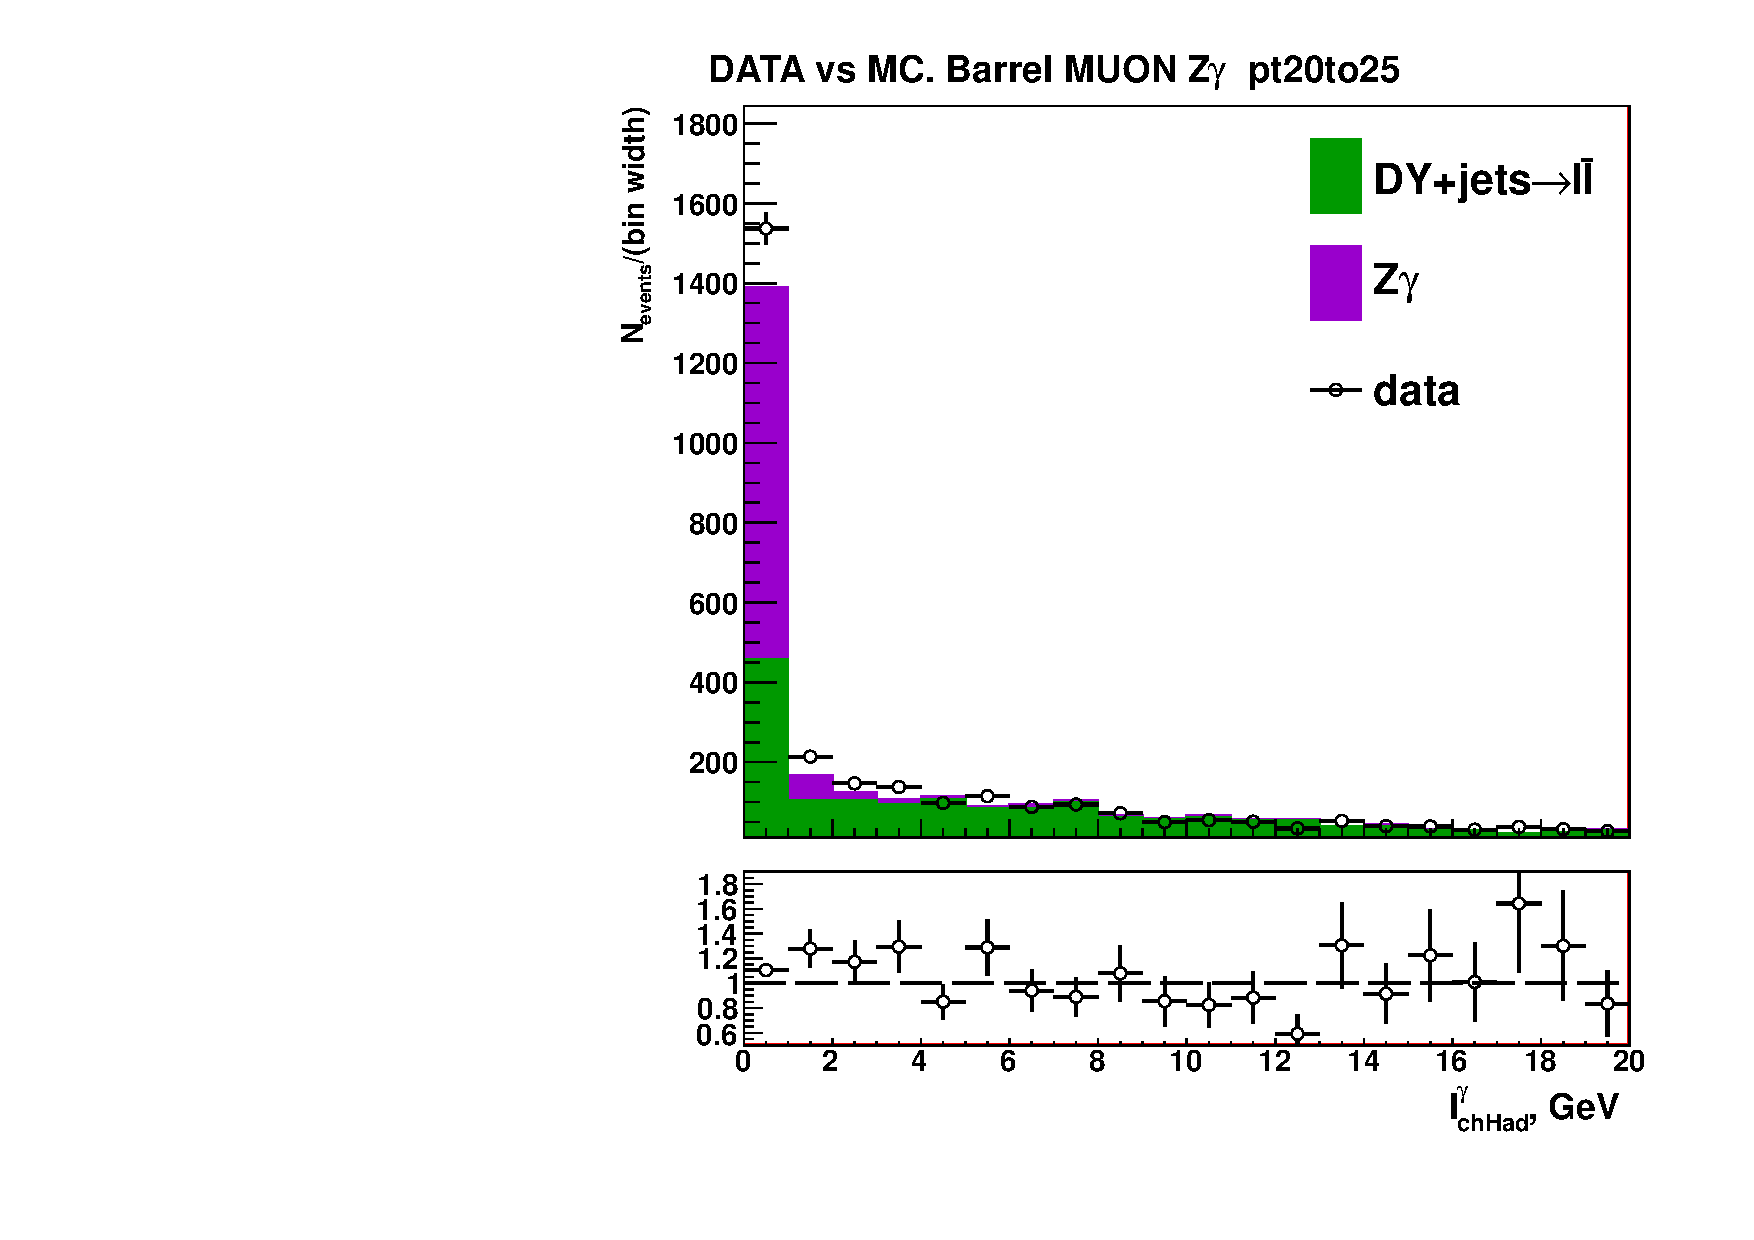
\includegraphics[width=0.32\textwidth]{../figs/figs_v11/MUON_ZGamma/PrepareYields/c_TotalDATAvsMC_Barrel__phoPFChIsoCorrFSR_EXCLUDED_pt20to25_.pdf}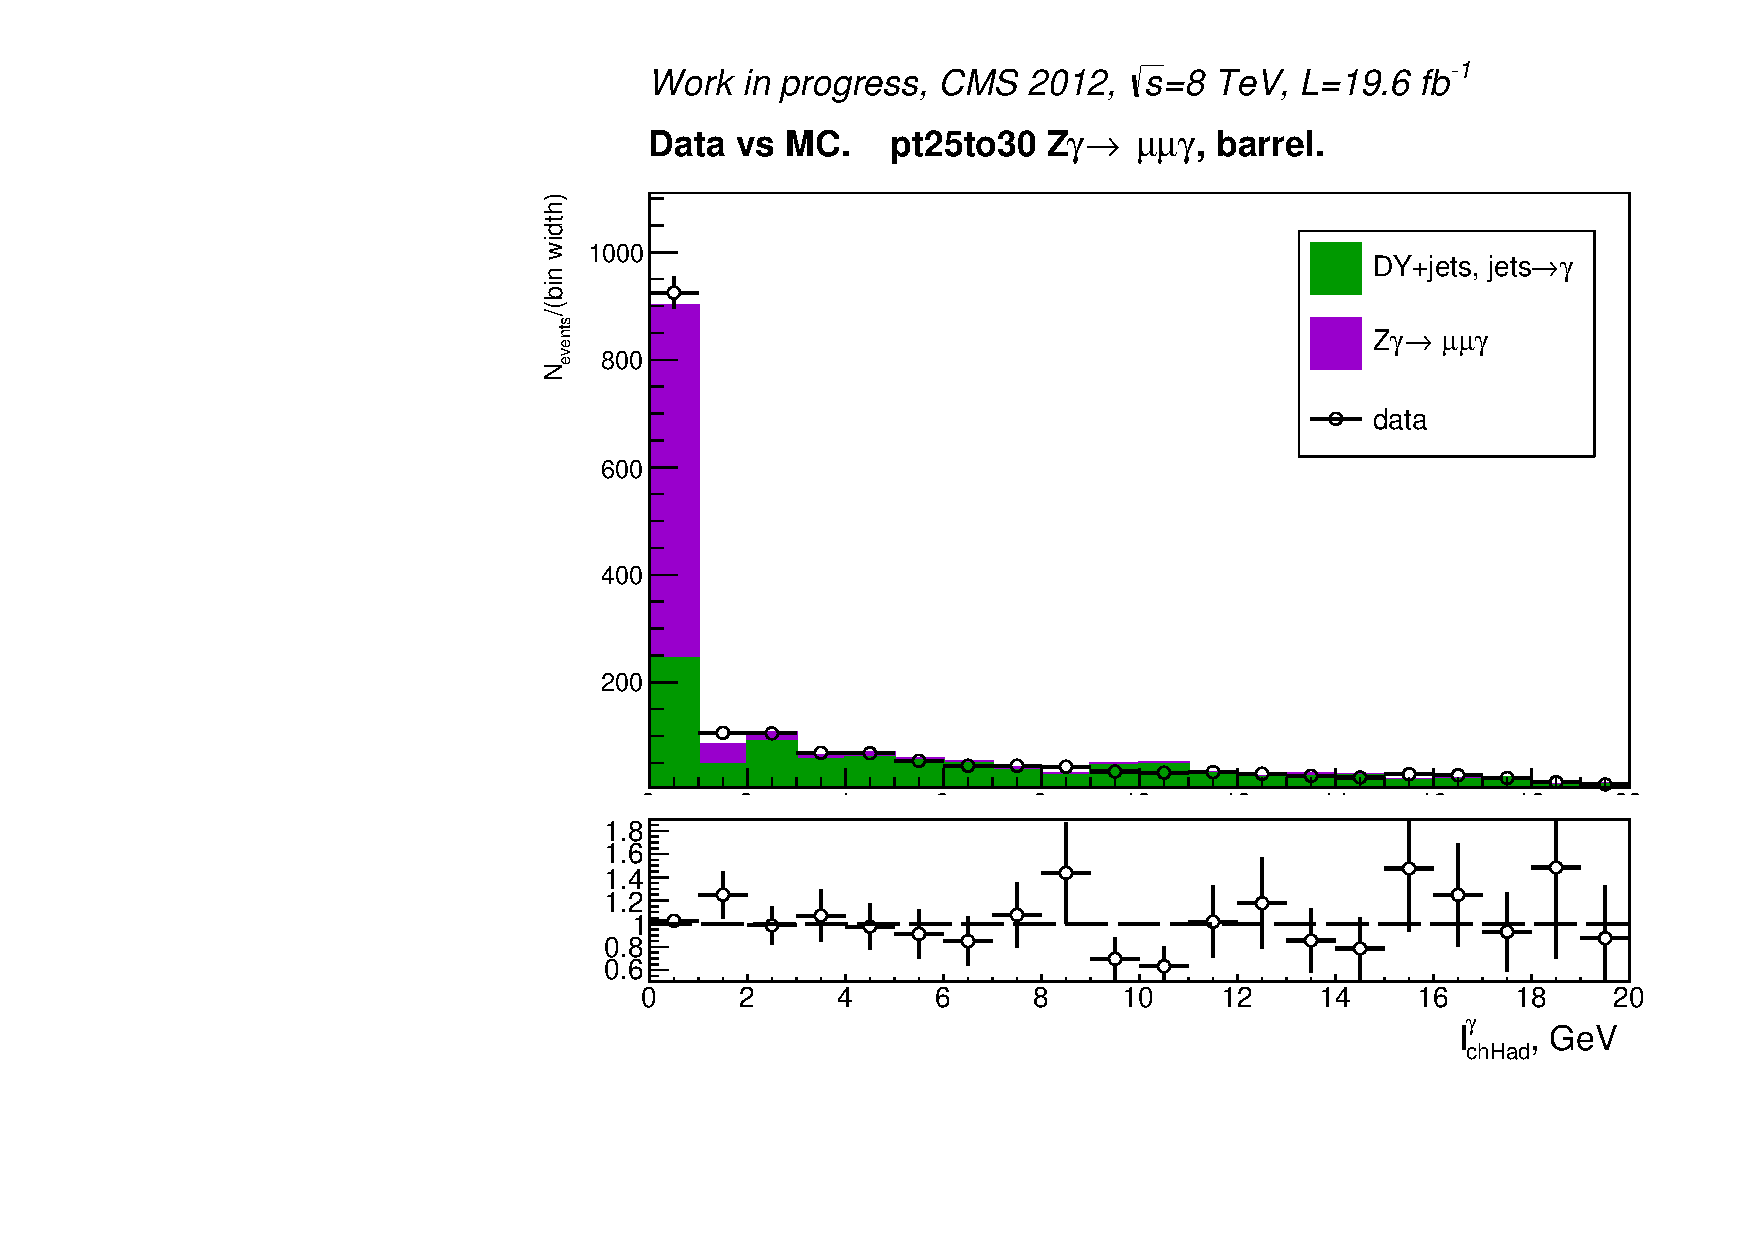
\includegraphics[width=0.32\textwidth]{../figs/figs_v11/MUON_ZGamma/PrepareYields/c_TotalDATAvsMC_Barrel__phoPFChIsoCorrFSR_EXCLUDED_pt25to30_.pdf}\\
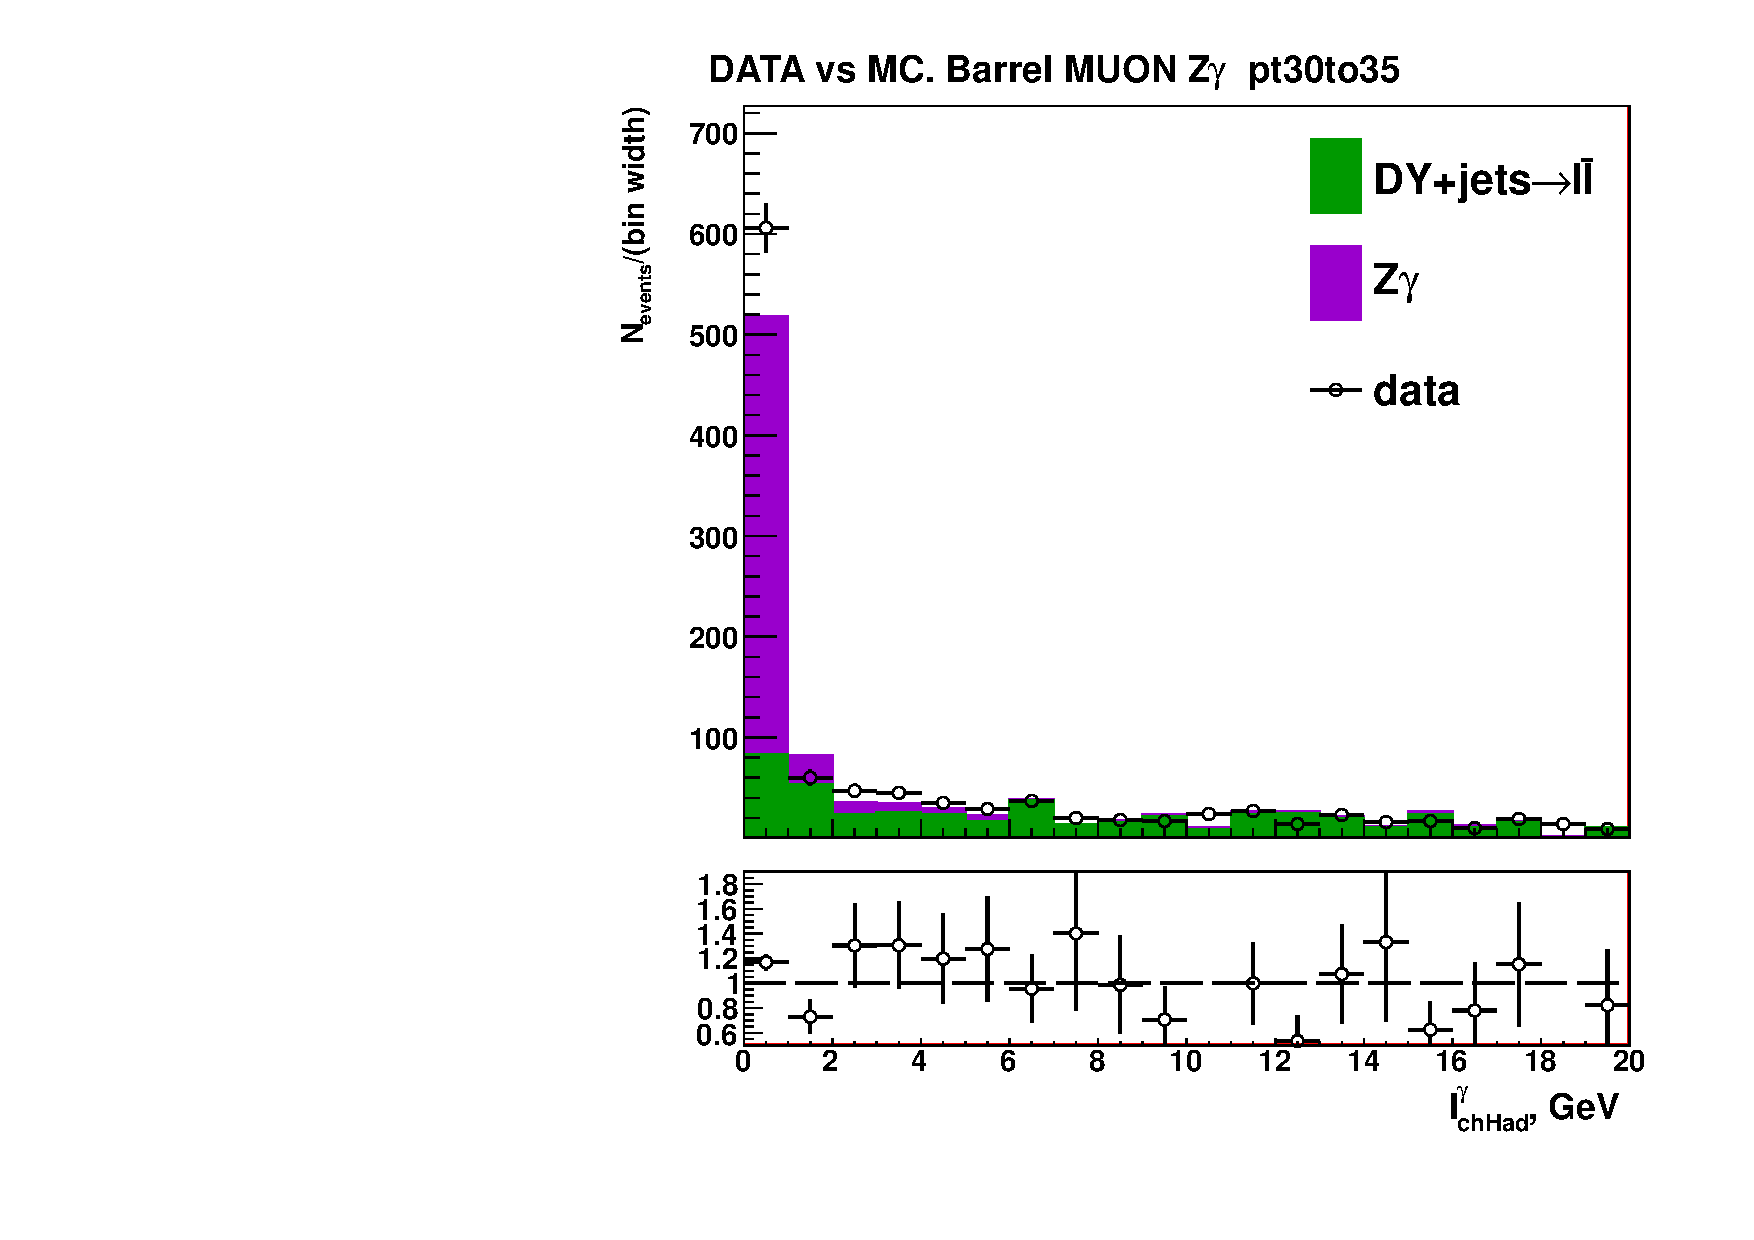
\includegraphics[width=0.32\textwidth]{../figs/figs_v11/MUON_ZGamma/PrepareYields/c_TotalDATAvsMC_Barrel__phoPFChIsoCorrFSR_EXCLUDED_pt30to35_.pdf}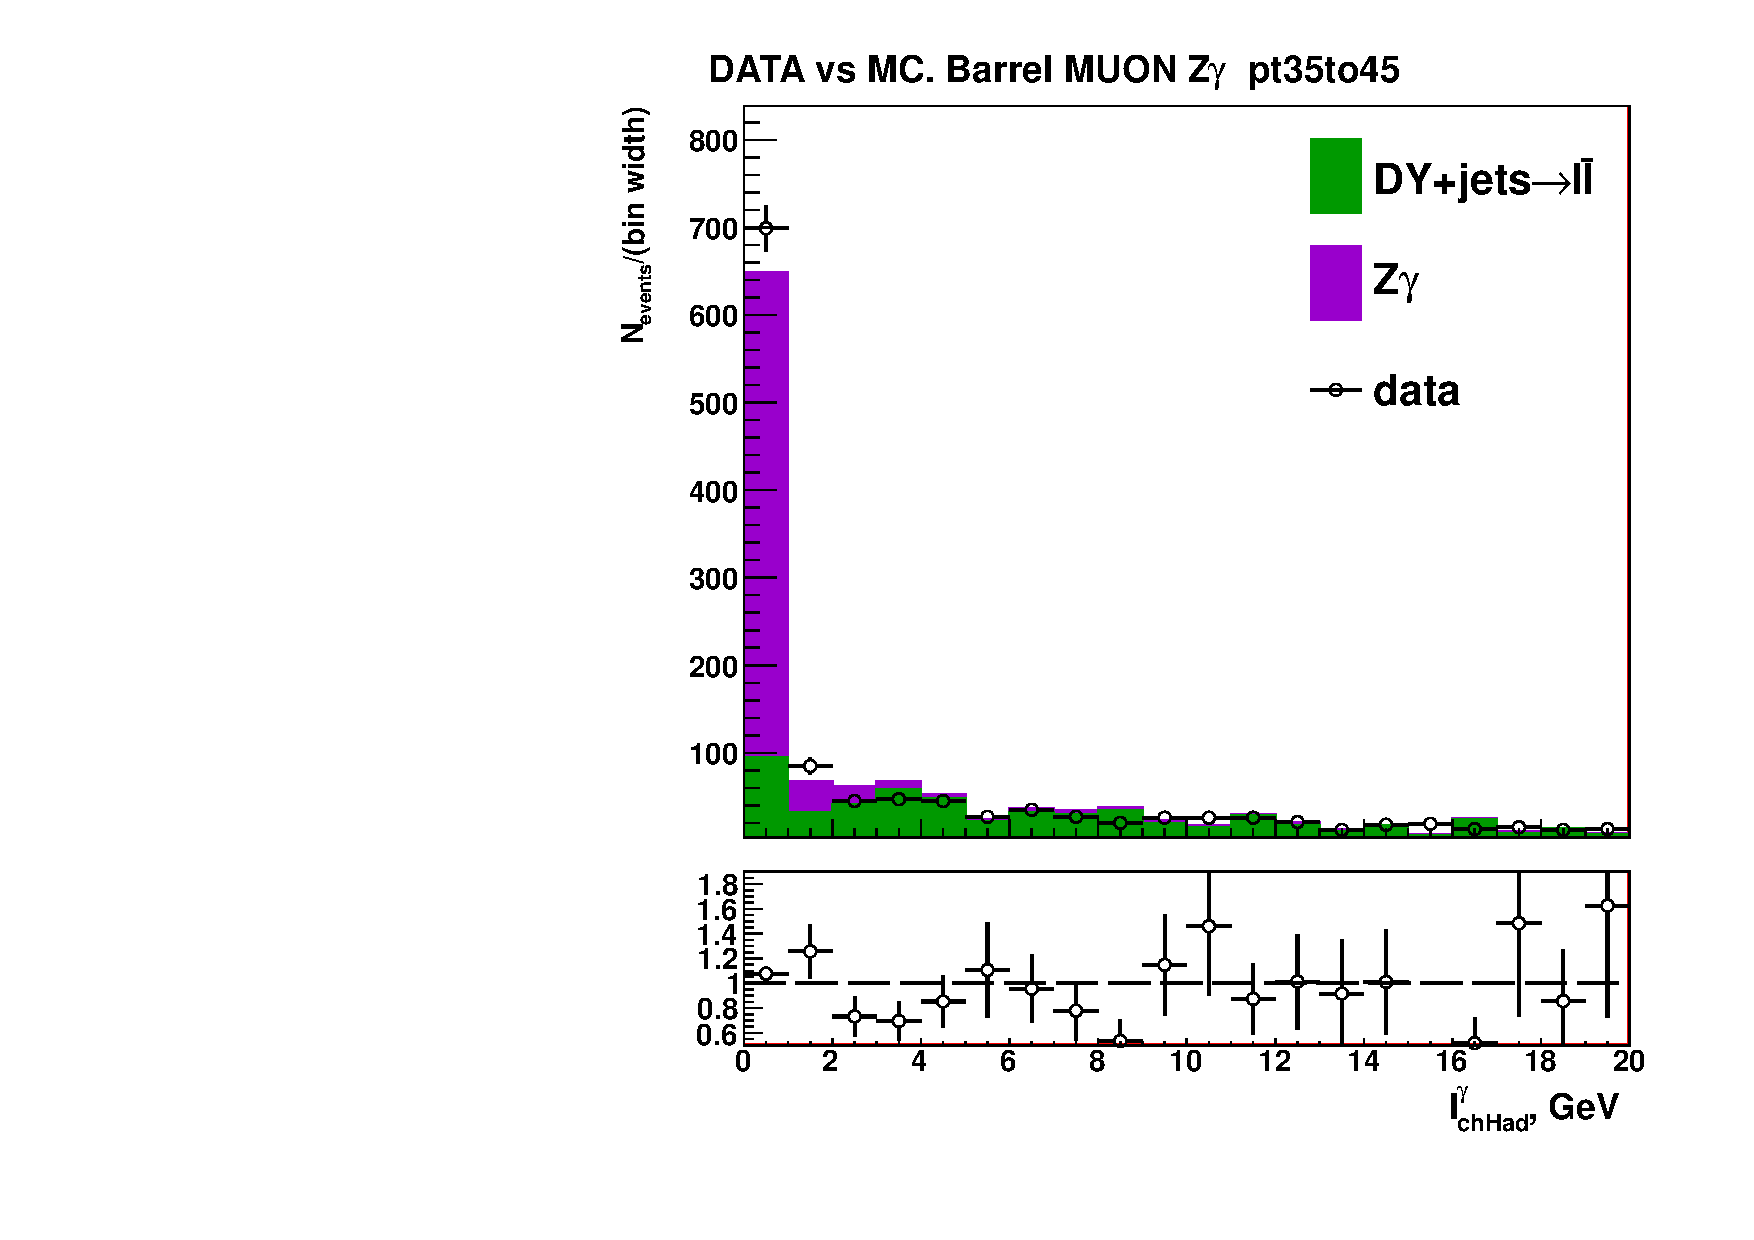
\includegraphics[width=0.32\textwidth]{../figs/figs_v11/MUON_ZGamma/PrepareYields/c_TotalDATAvsMC_Barrel__phoPFChIsoCorrFSR_EXCLUDED_pt35to45_.pdf}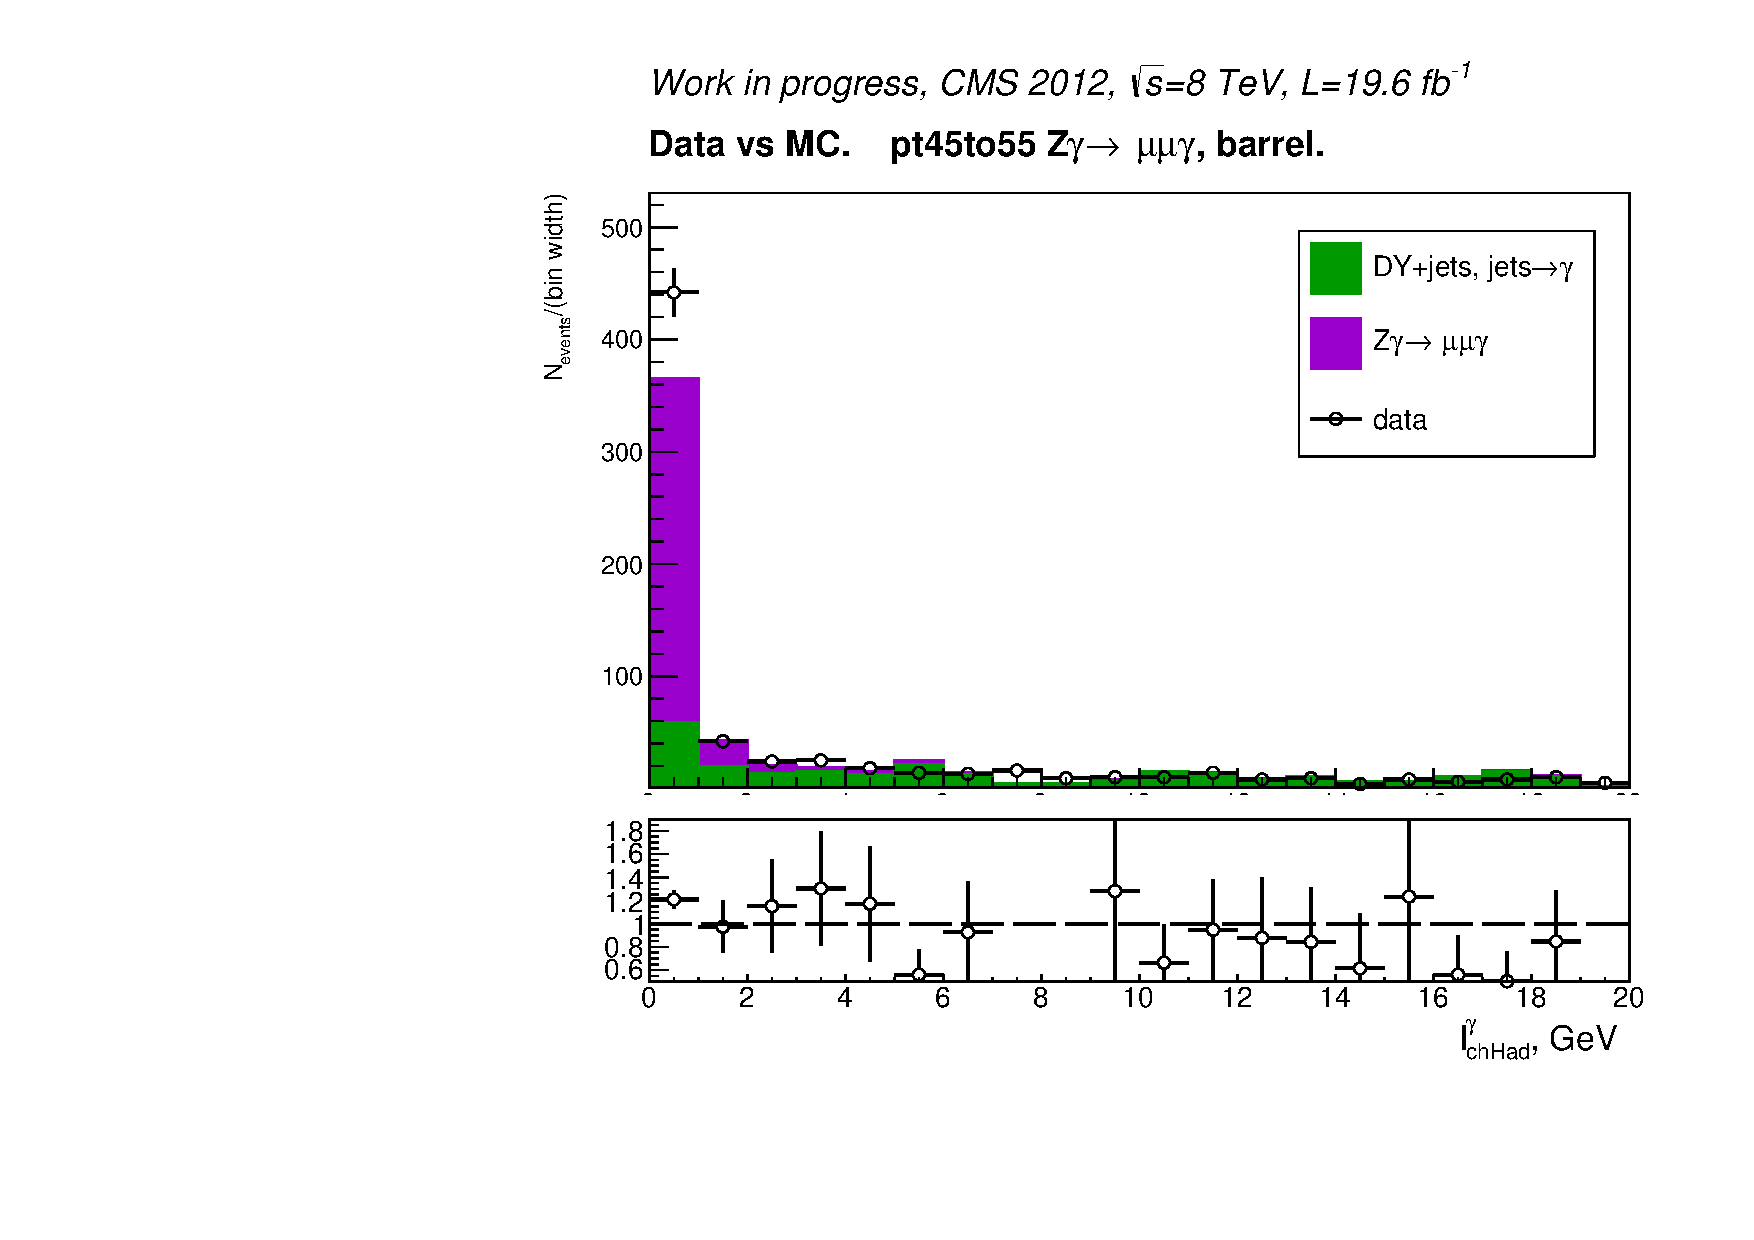
\includegraphics[width=0.32\textwidth]{../figs/figs_v11/MUON_ZGamma/PrepareYields/c_TotalDATAvsMC_Barrel__phoPFChIsoCorrFSR_EXCLUDED_pt45to55_.pdf}\\
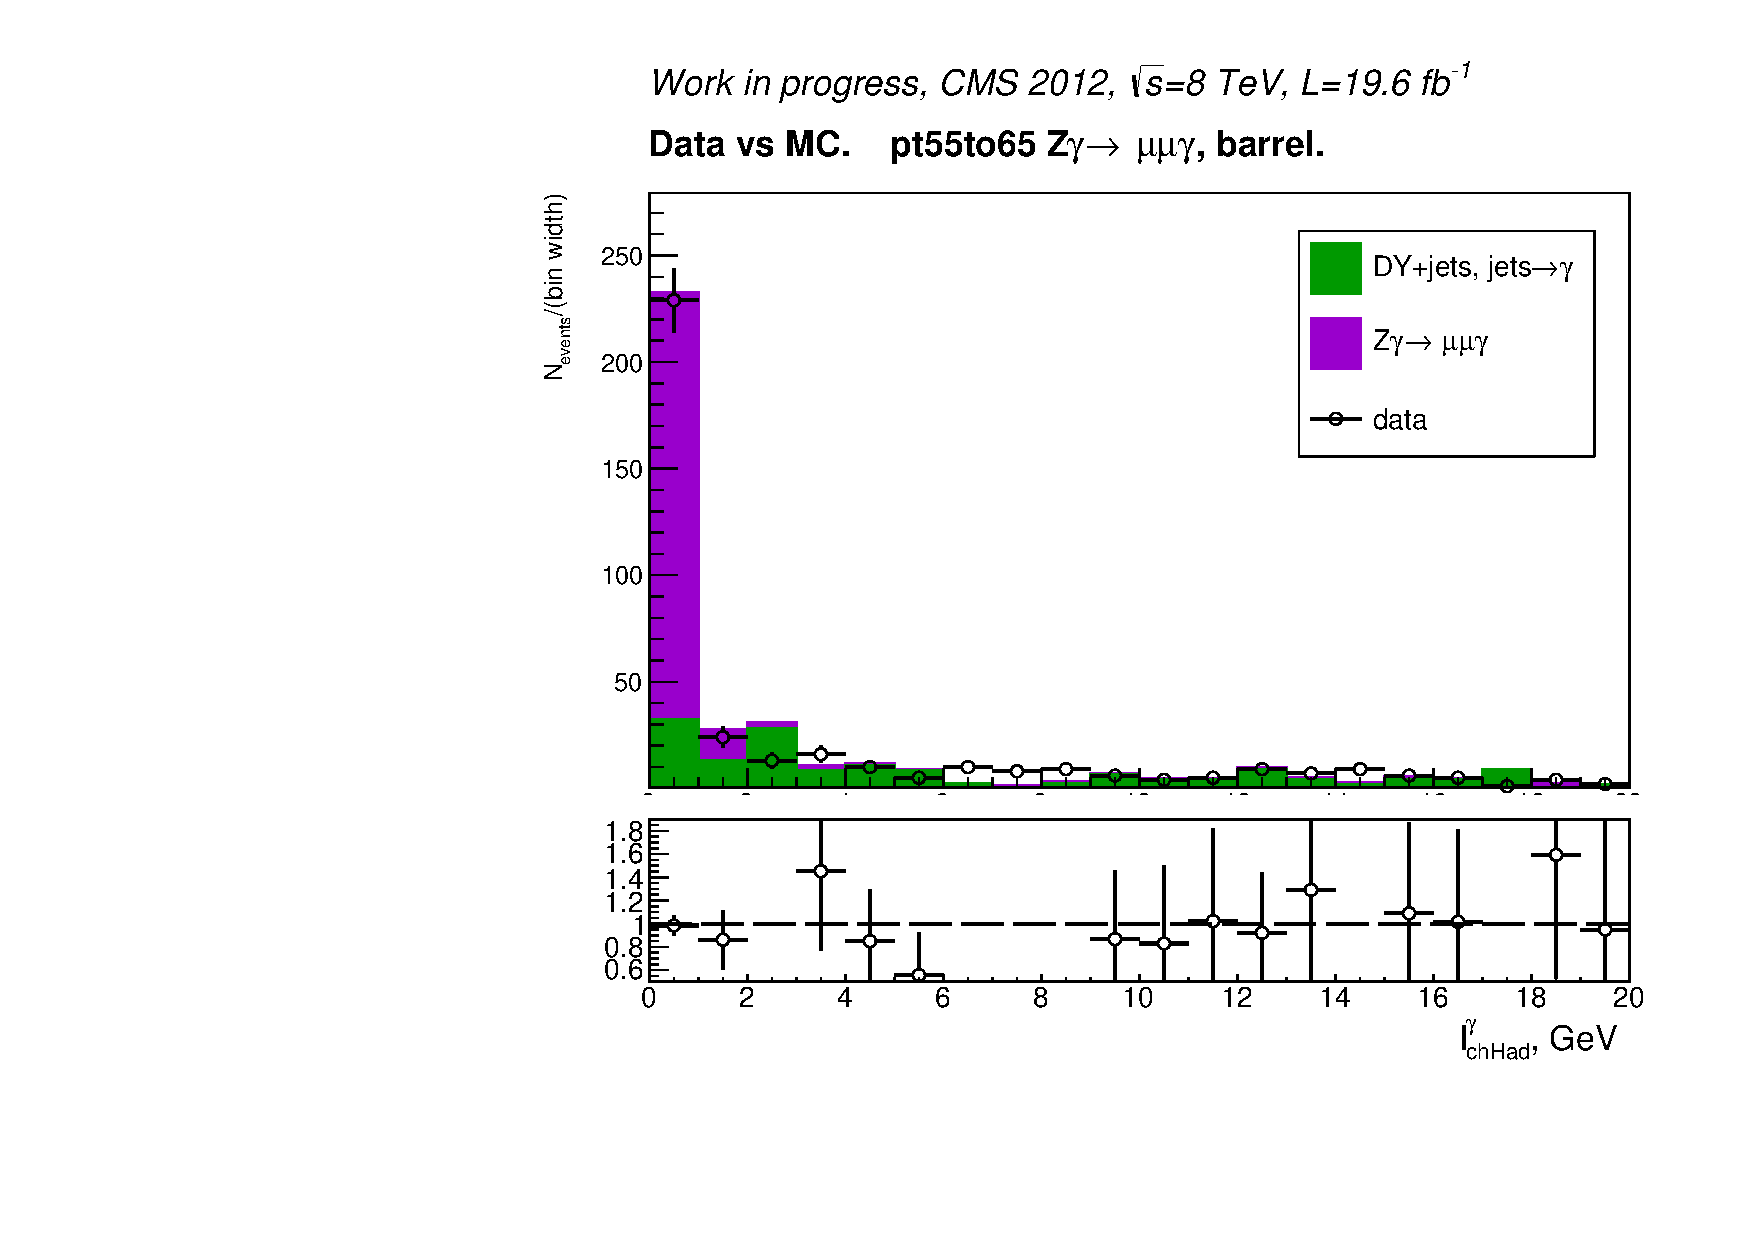
\includegraphics[width=0.32\textwidth]{../figs/figs_v11/MUON_ZGamma/PrepareYields/c_TotalDATAvsMC_Barrel__phoPFChIsoCorrFSR_EXCLUDED_pt55to65_.pdf}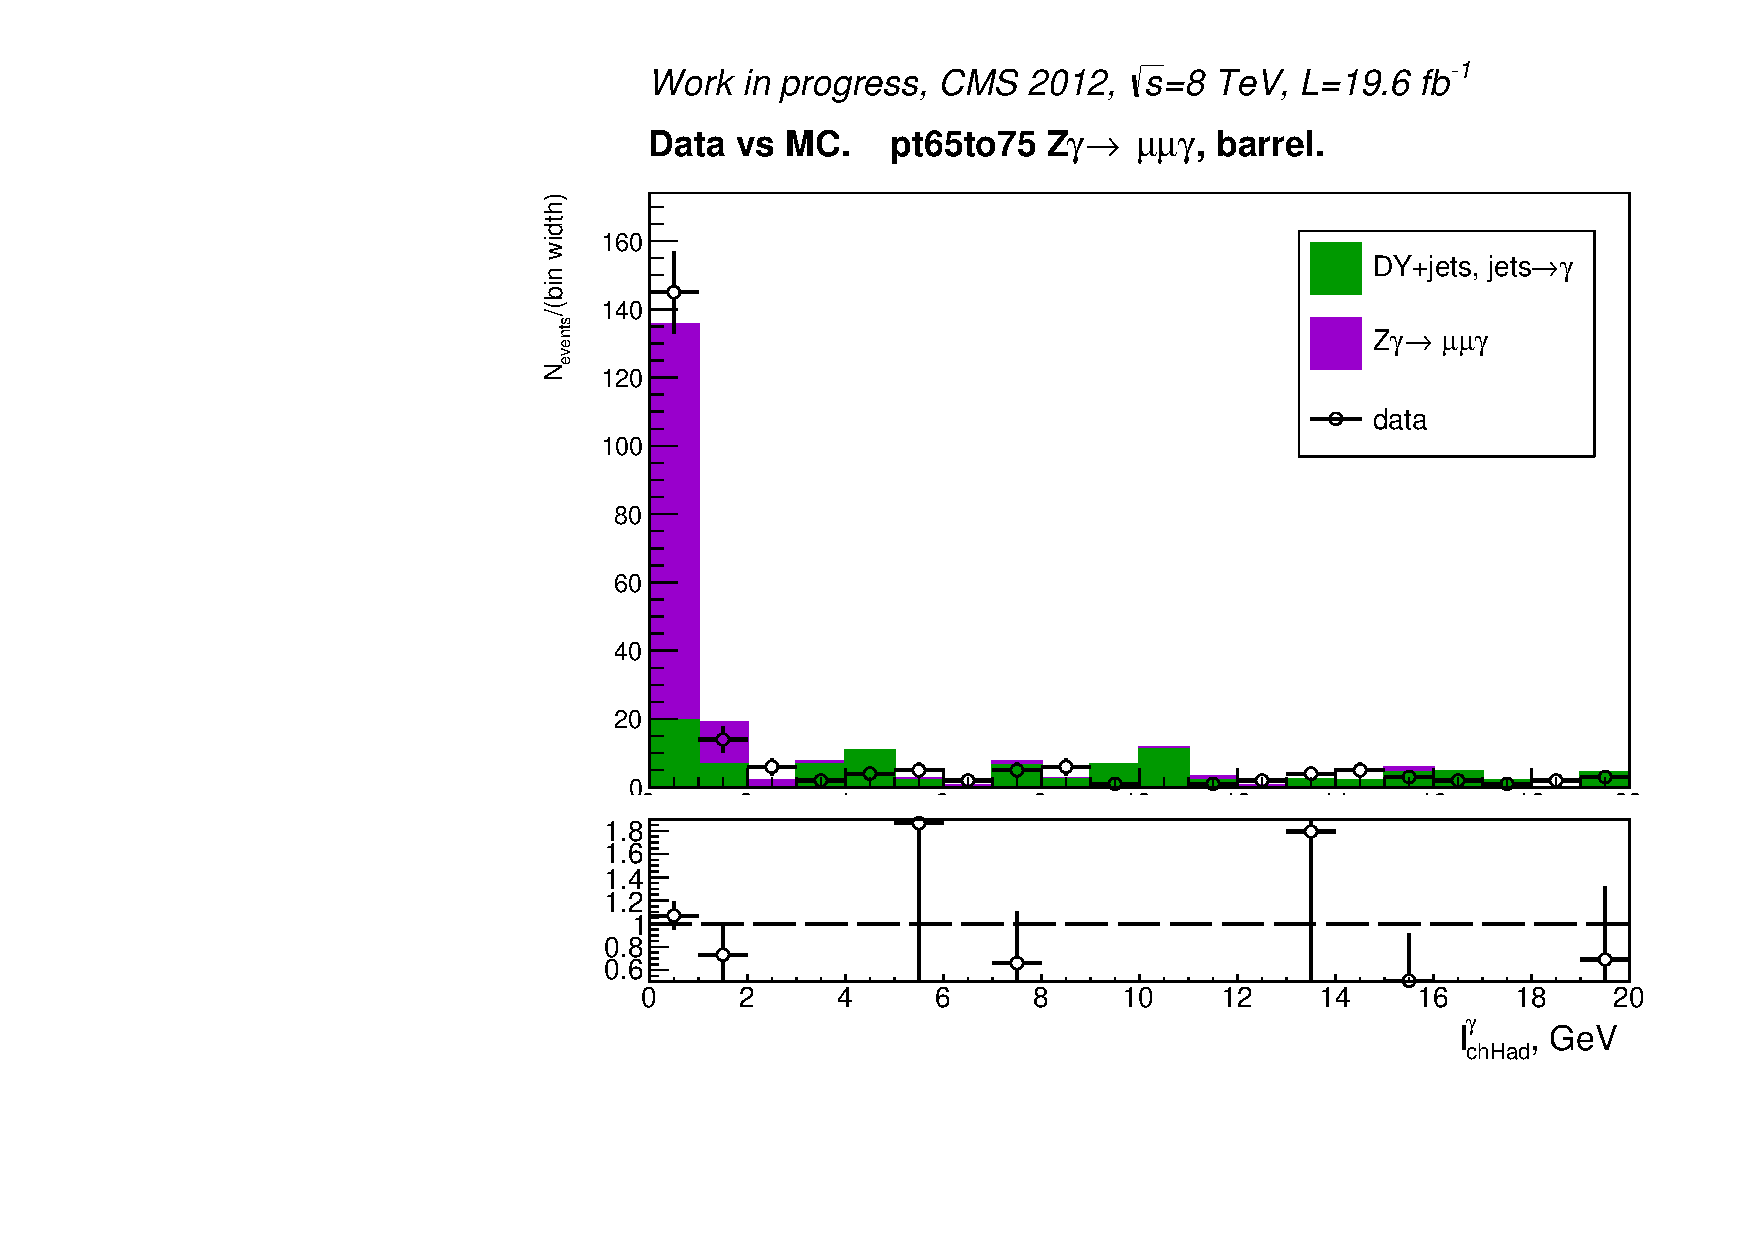
\includegraphics[width=0.32\textwidth]{../figs/figs_v11/MUON_ZGamma/PrepareYields/c_TotalDATAvsMC_Barrel__phoPFChIsoCorrFSR_EXCLUDED_pt65to75_.pdf}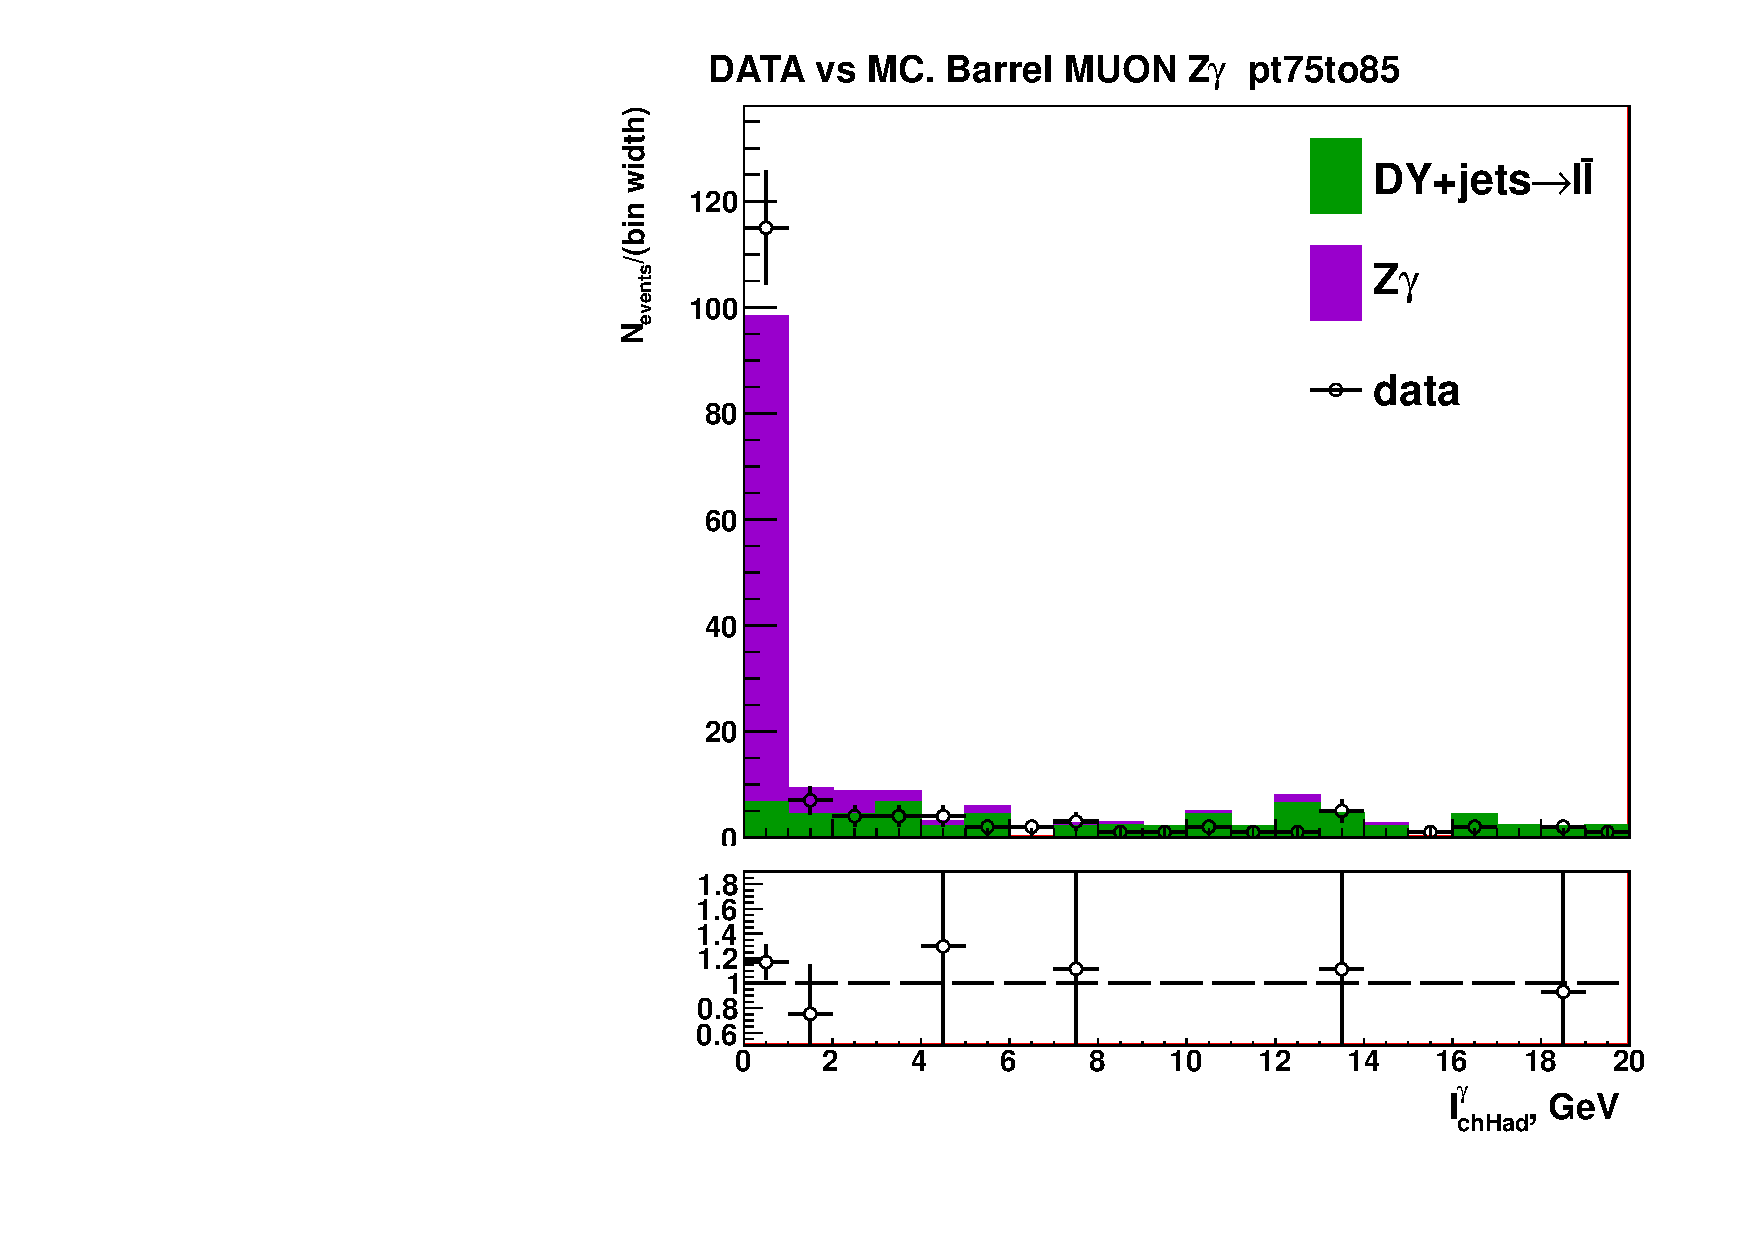
\includegraphics[width=0.32\textwidth]{../figs/figs_v11/MUON_ZGamma/PrepareYields/c_TotalDATAvsMC_Barrel__phoPFChIsoCorrFSR_EXCLUDED_pt75to85_.pdf}\\
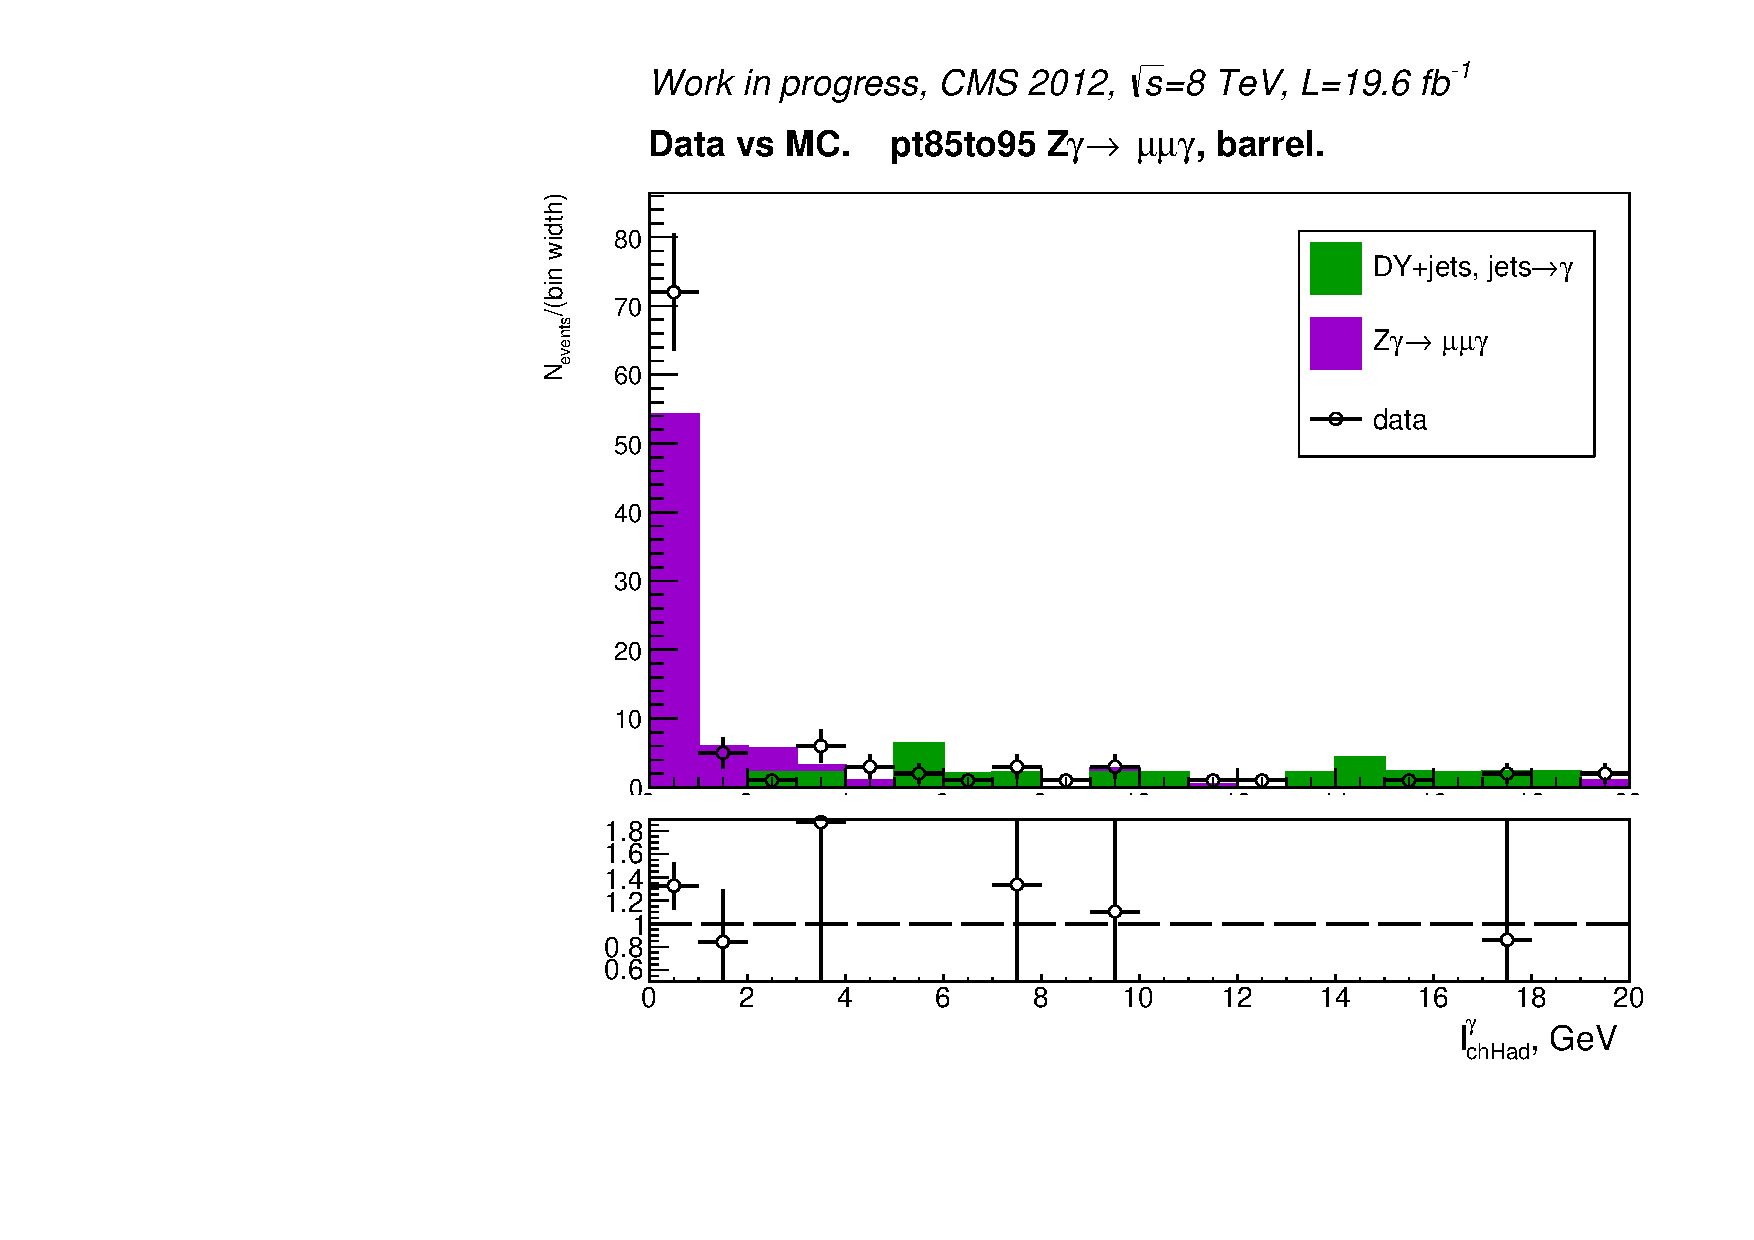
\includegraphics[width=0.32\textwidth]{../figs/figs_v11/MUON_ZGamma/PrepareYields/c_TotalDATAvsMC_Barrel__phoPFChIsoCorrFSR_EXCLUDED_pt85to95_.pdf}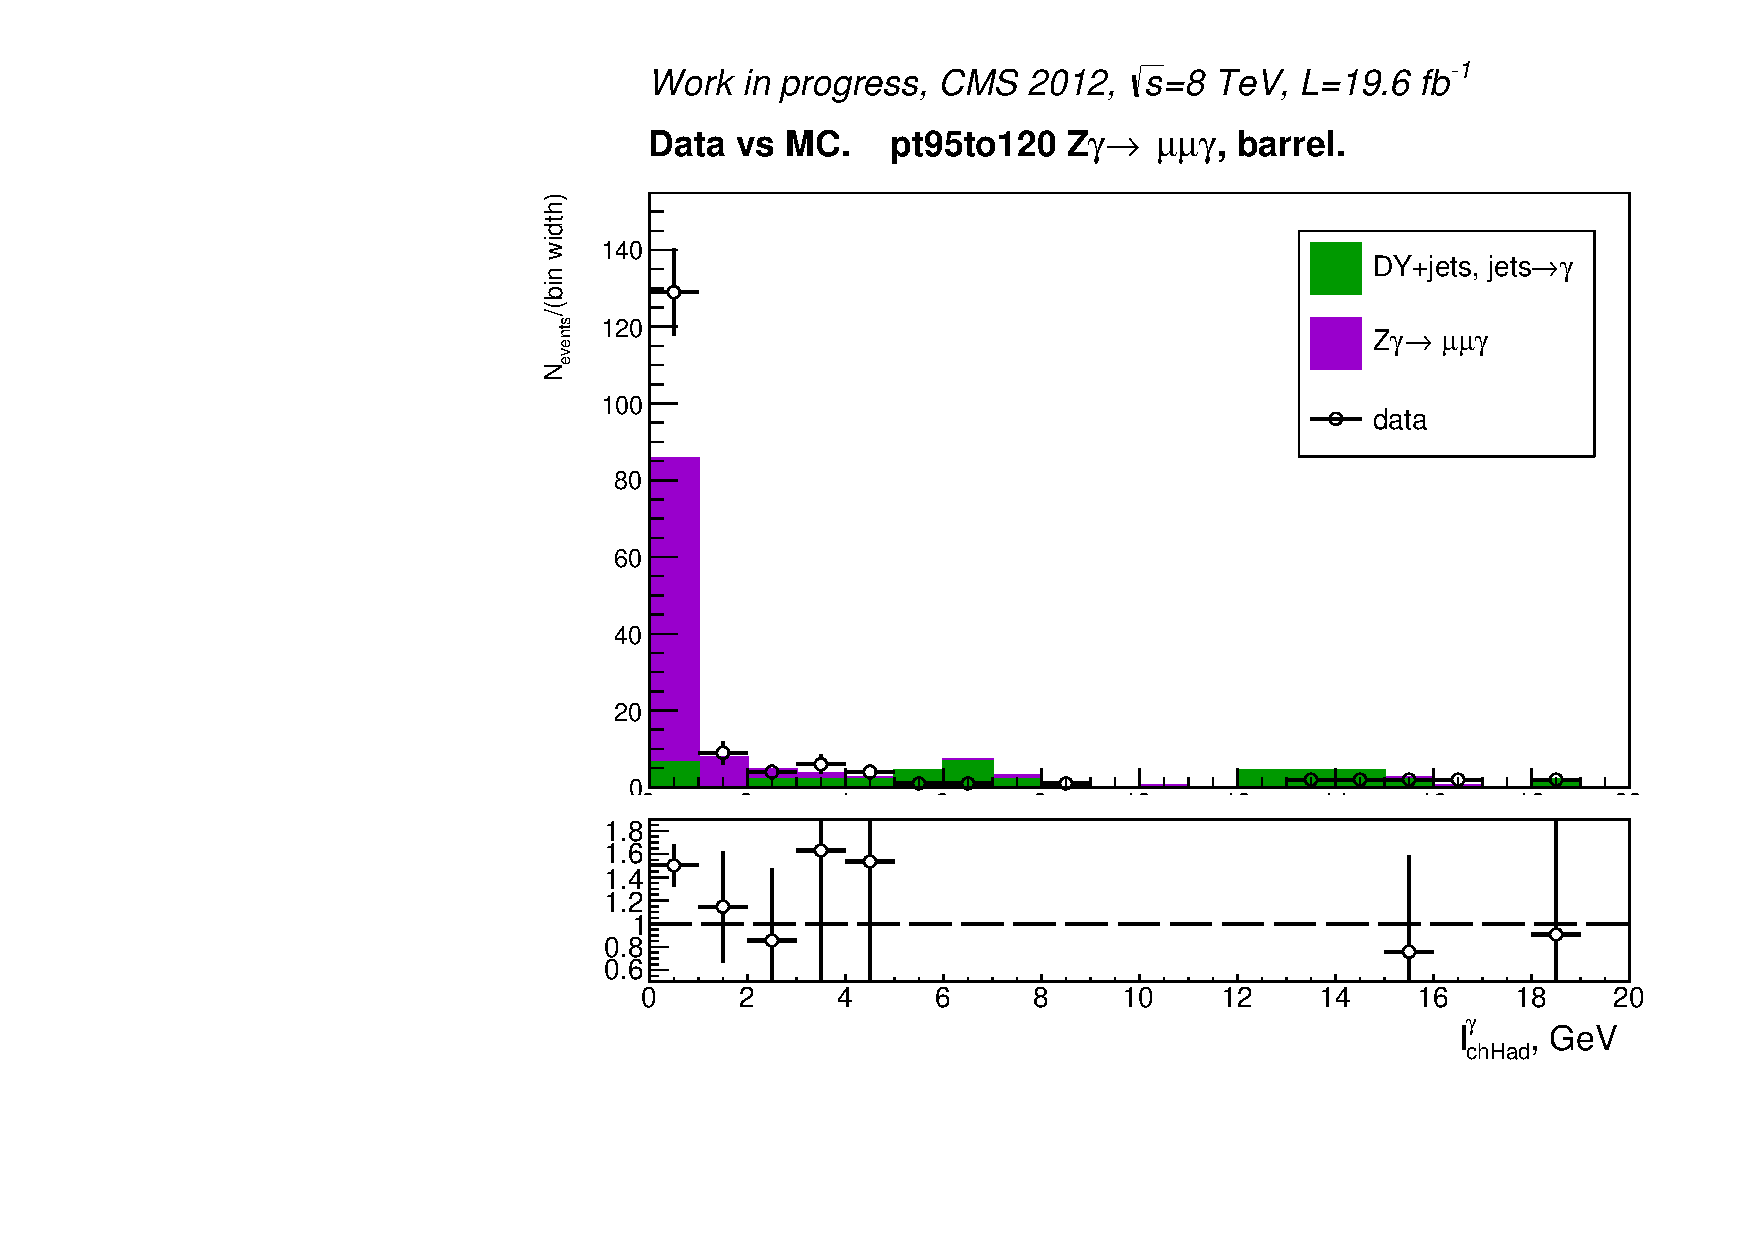
\includegraphics[width=0.32\textwidth]{../figs/figs_v11/MUON_ZGamma/PrepareYields/c_TotalDATAvsMC_Barrel__phoPFChIsoCorrFSR_EXCLUDED_pt95to120_.pdf}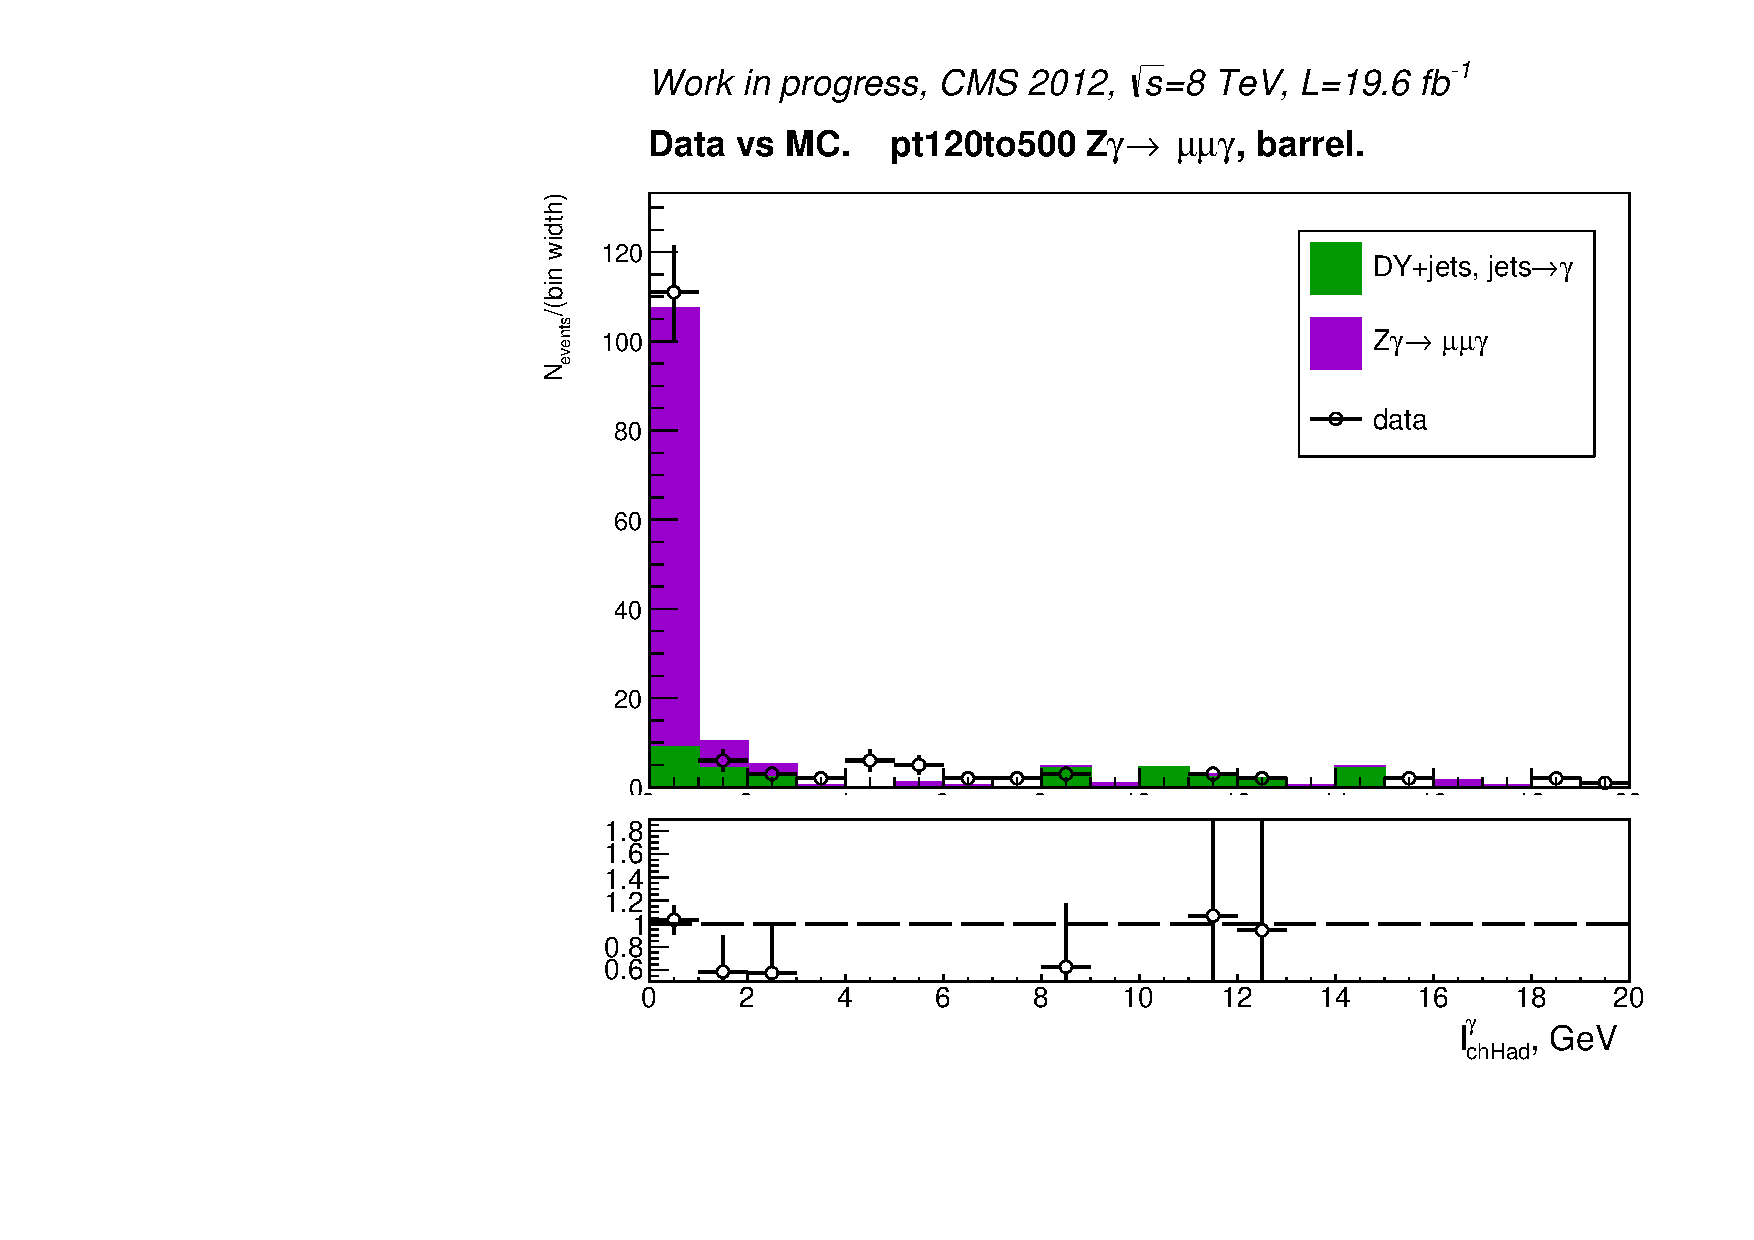
\includegraphics[width=0.32\textwidth]{../figs/figs_v11/MUON_ZGamma/PrepareYields/c_TotalDATAvsMC_Barrel__phoPFChIsoCorrFSR_EXCLUDED_pt120to500_.pdf}\\
  \caption{$Z\gamma$-selected ISR events, data vs MC. Distributions of $I_{chHad}^{\gamma}$ used for preparing fake-$\gamma$ templates. Real-$\gamma$ contribution to ISR region is subtracted based on $Z\gamma$ signal MC prediction to prepare fake-$\gamma$ templates. Ranges of $<P_T^{\gamma}$ are shown in the plot titles and cover the total range of 15~GeV$<P_T^{\gamma}<$500~GeV. EB photons. }
  \label{fig:Zg_ISR_phoPFChIsoCorr_Barrel}
  \end{center}
\end{figure}

\begin{figure}[htb]
  \begin{center}
   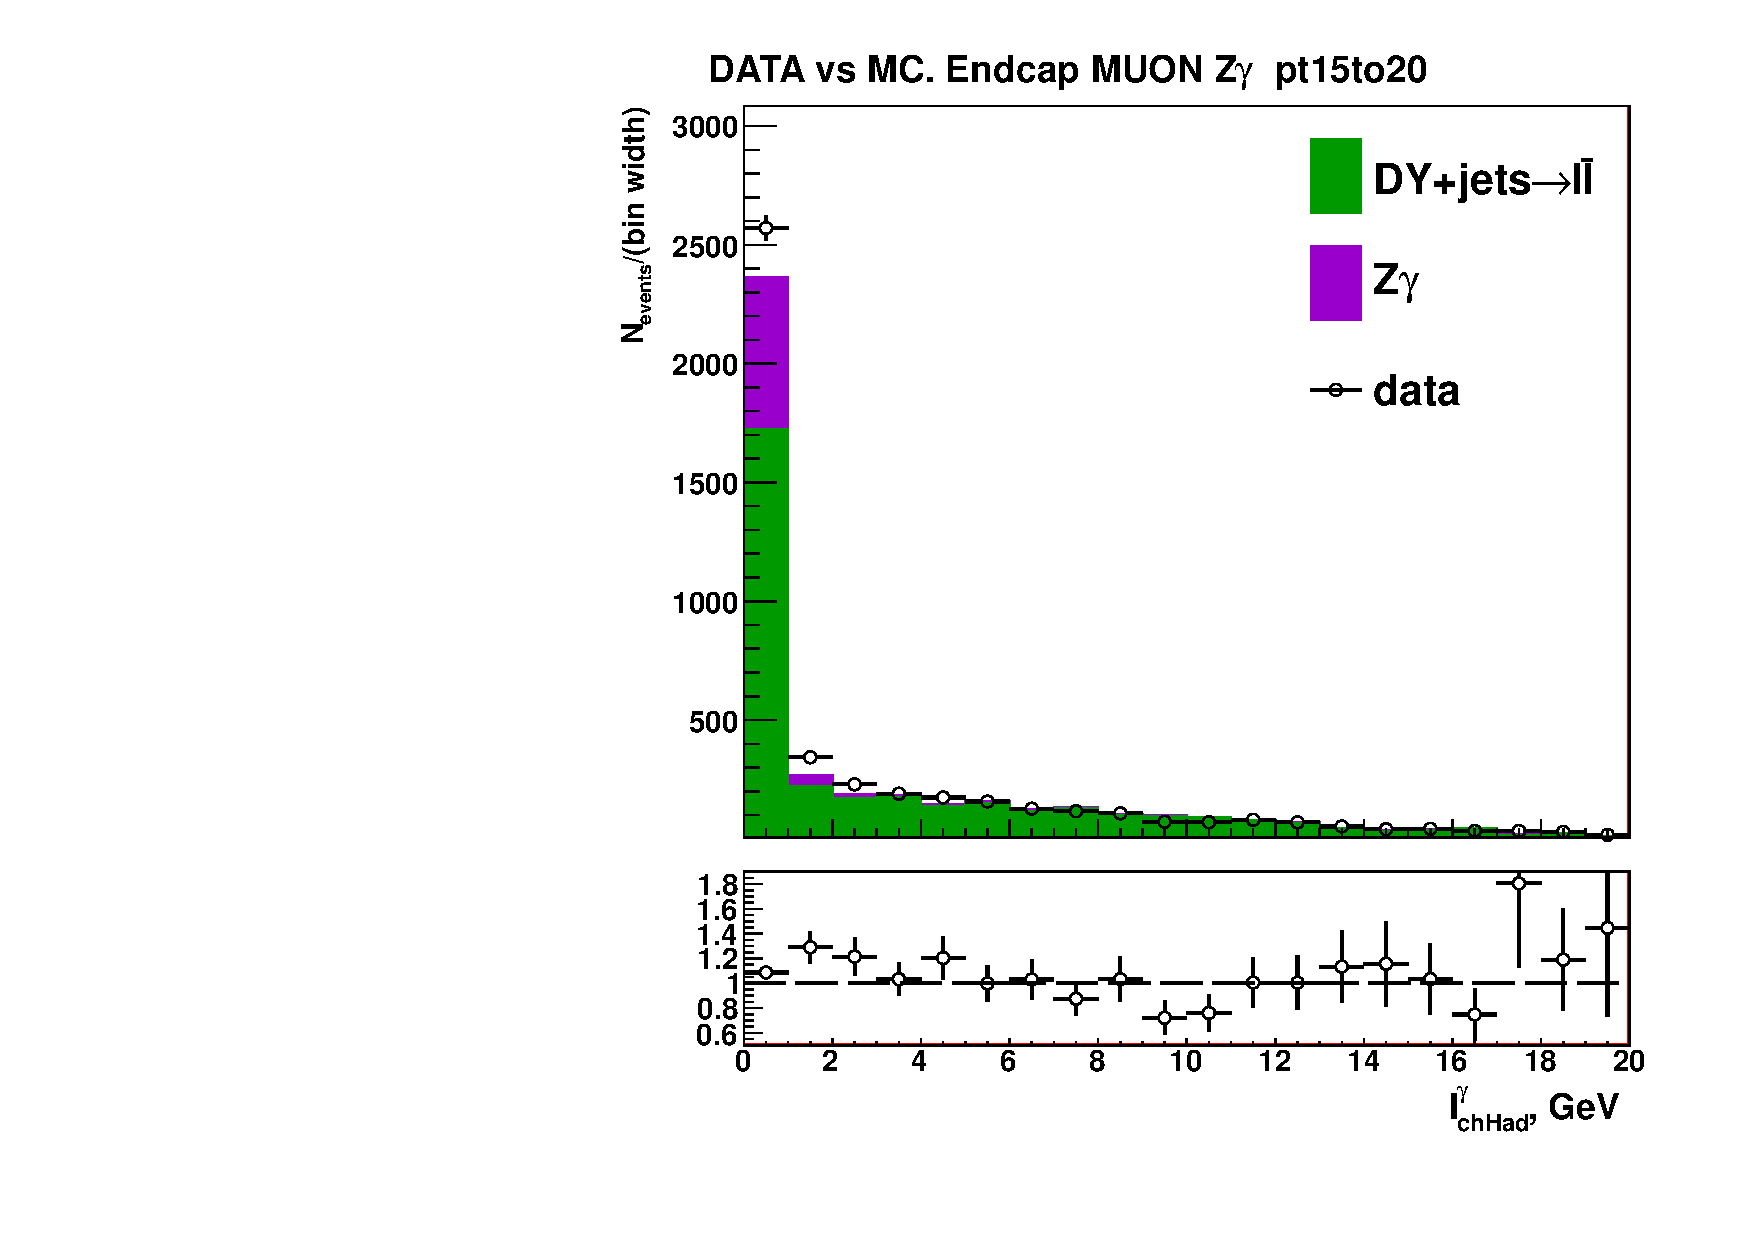
\includegraphics[width=0.32\textwidth]{../figs/figs_v11/MUON_ZGamma/PrepareYields/c_TotalDATAvsMC_Endcap__phoPFChIsoCorrFSR_EXCLUDED_pt15to20_.pdf}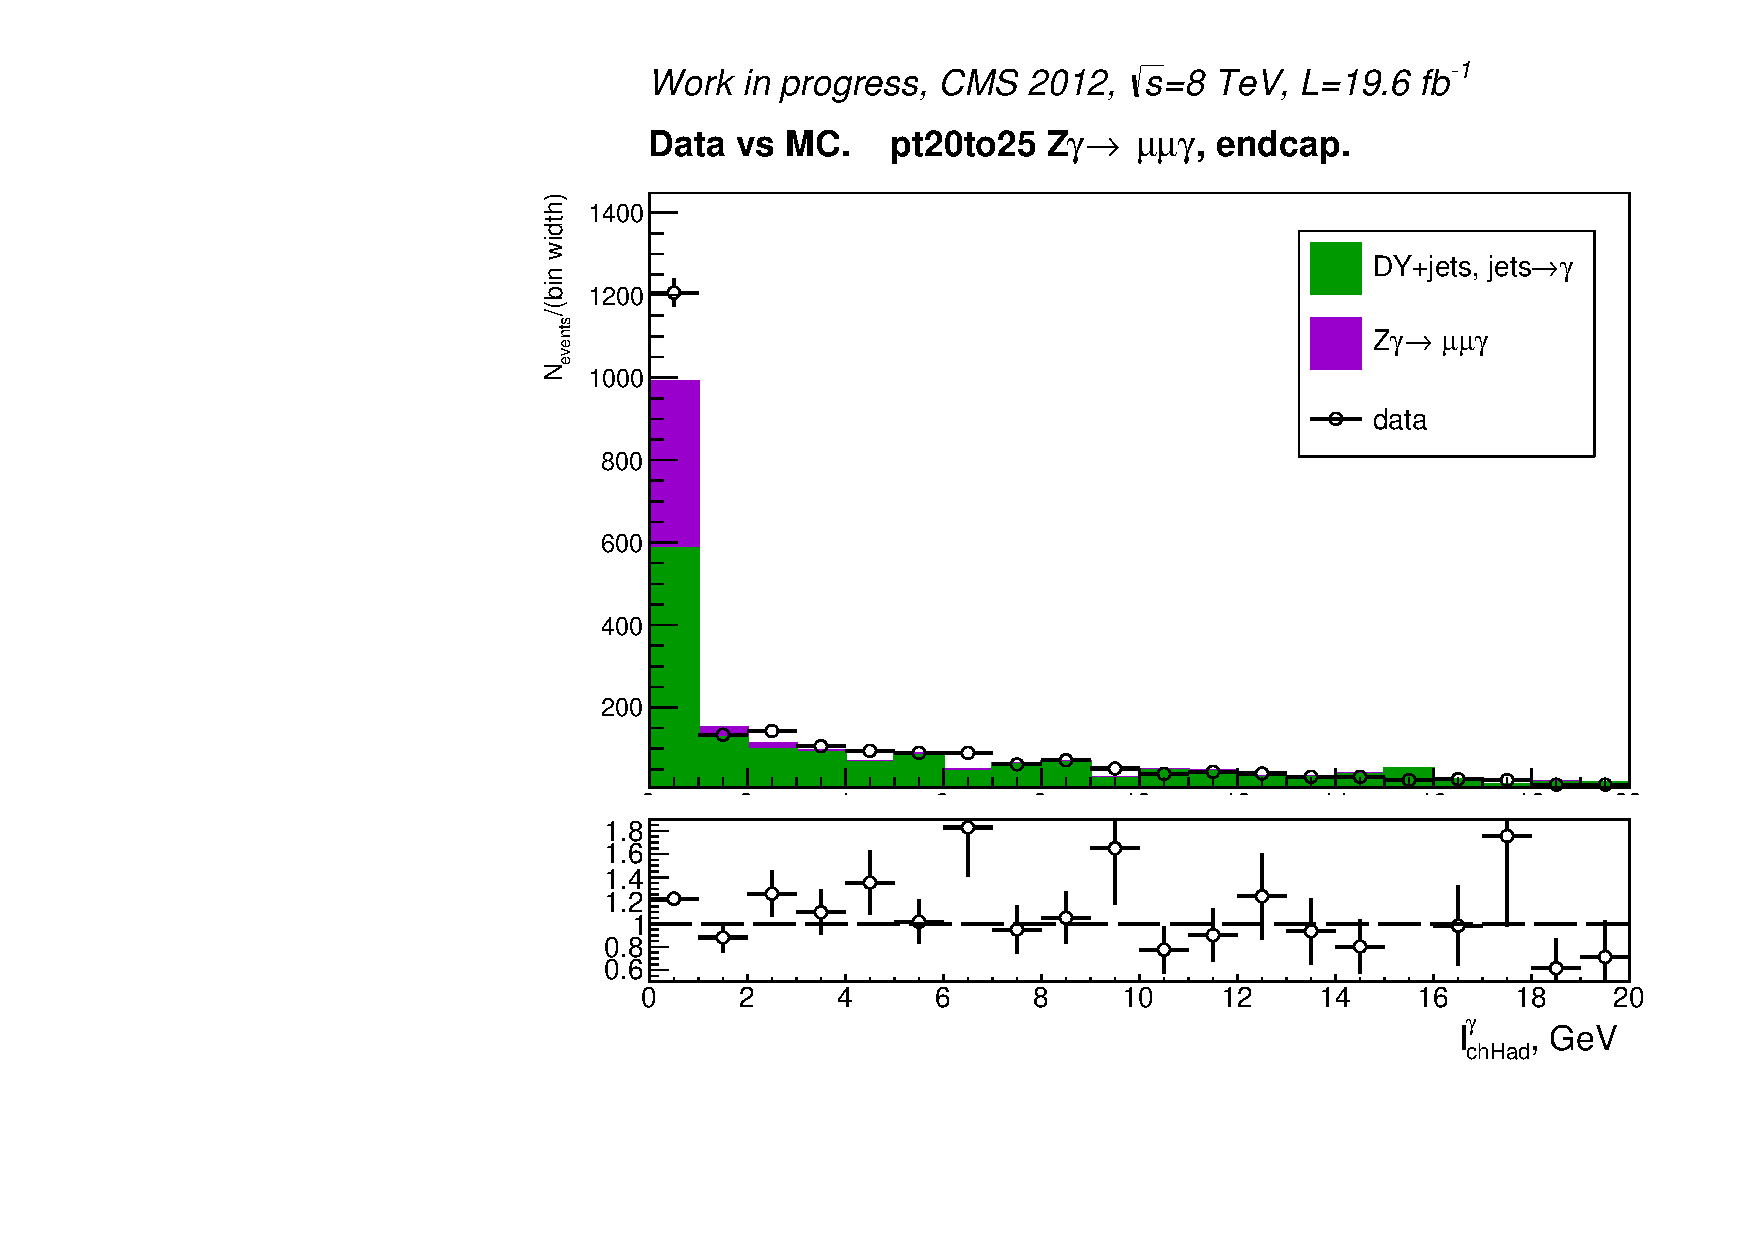
\includegraphics[width=0.32\textwidth]{../figs/figs_v11/MUON_ZGamma/PrepareYields/c_TotalDATAvsMC_Endcap__phoPFChIsoCorrFSR_EXCLUDED_pt20to25_.pdf}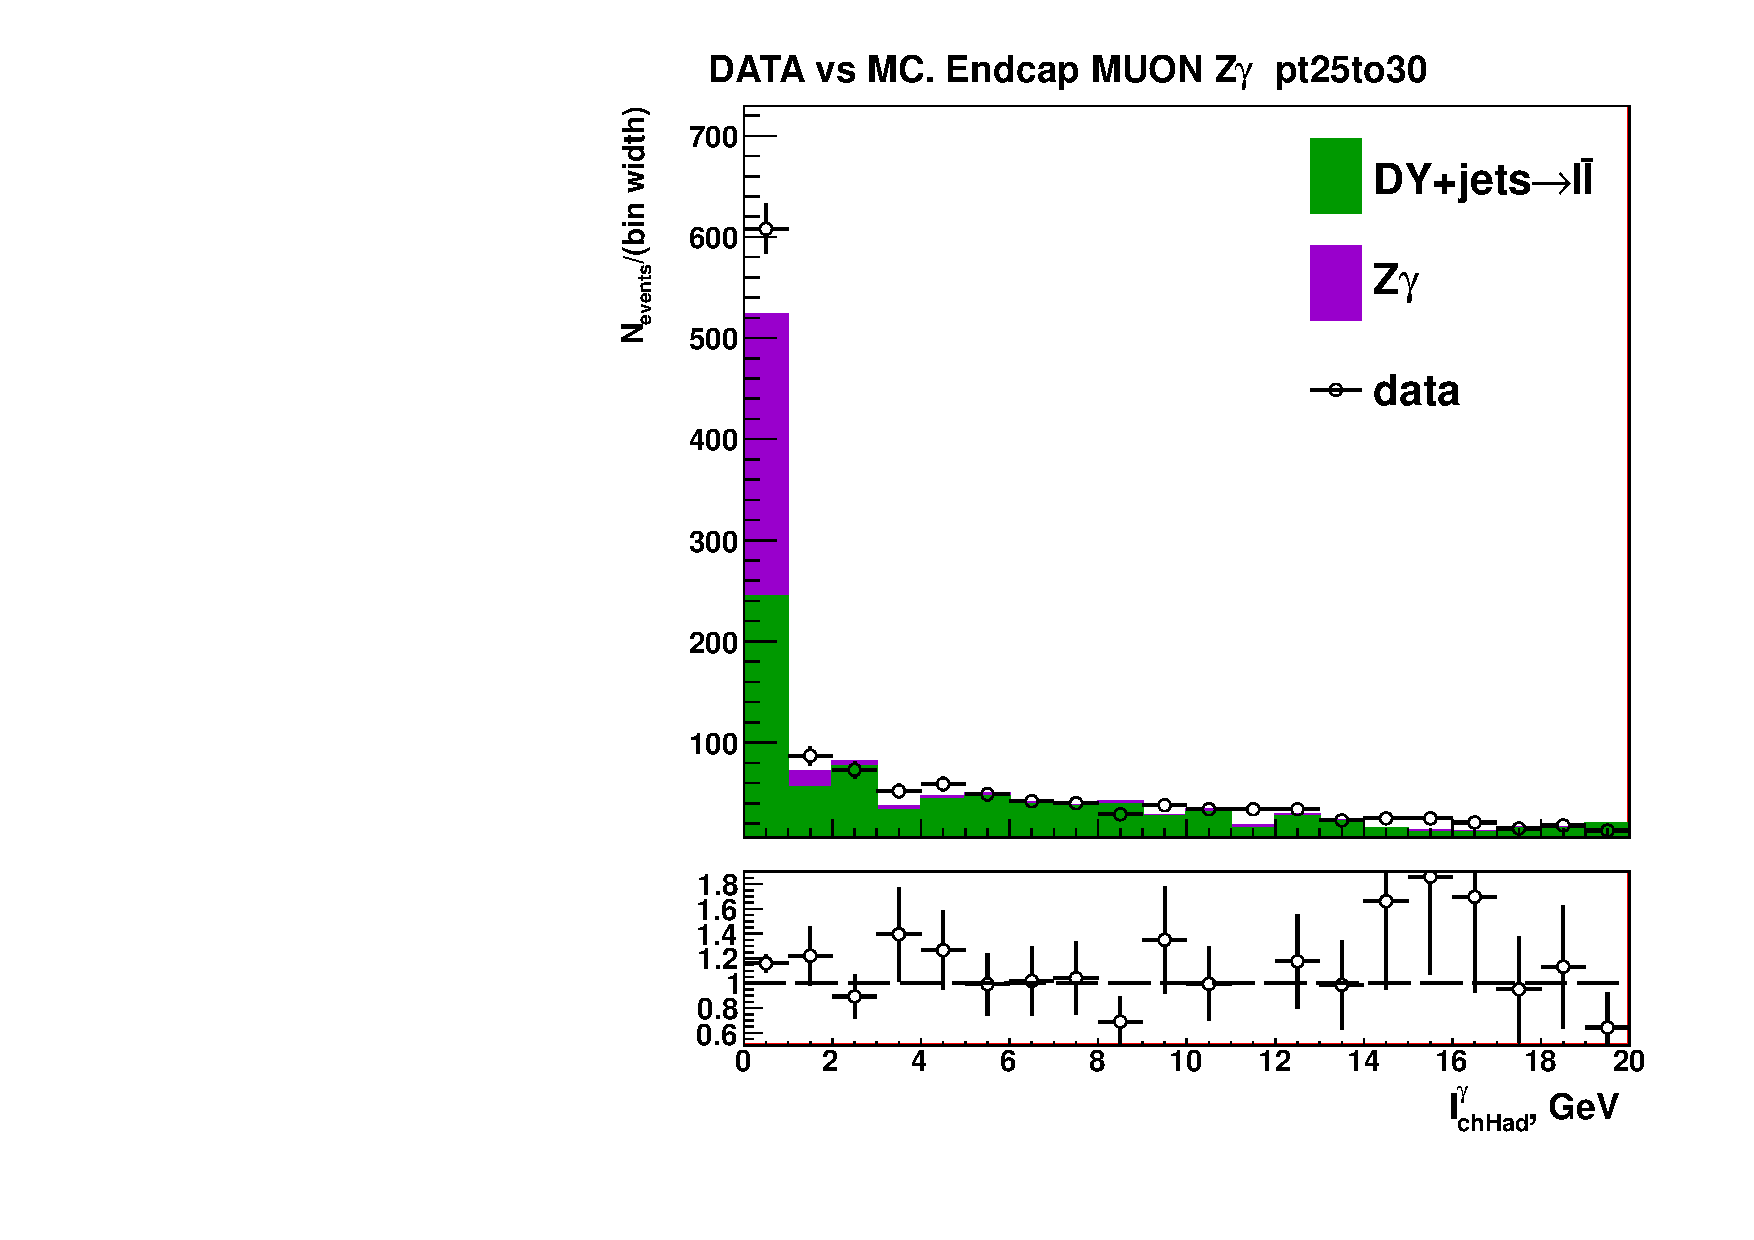
\includegraphics[width=0.32\textwidth]{../figs/figs_v11/MUON_ZGamma/PrepareYields/c_TotalDATAvsMC_Endcap__phoPFChIsoCorrFSR_EXCLUDED_pt25to30_.pdf}\\
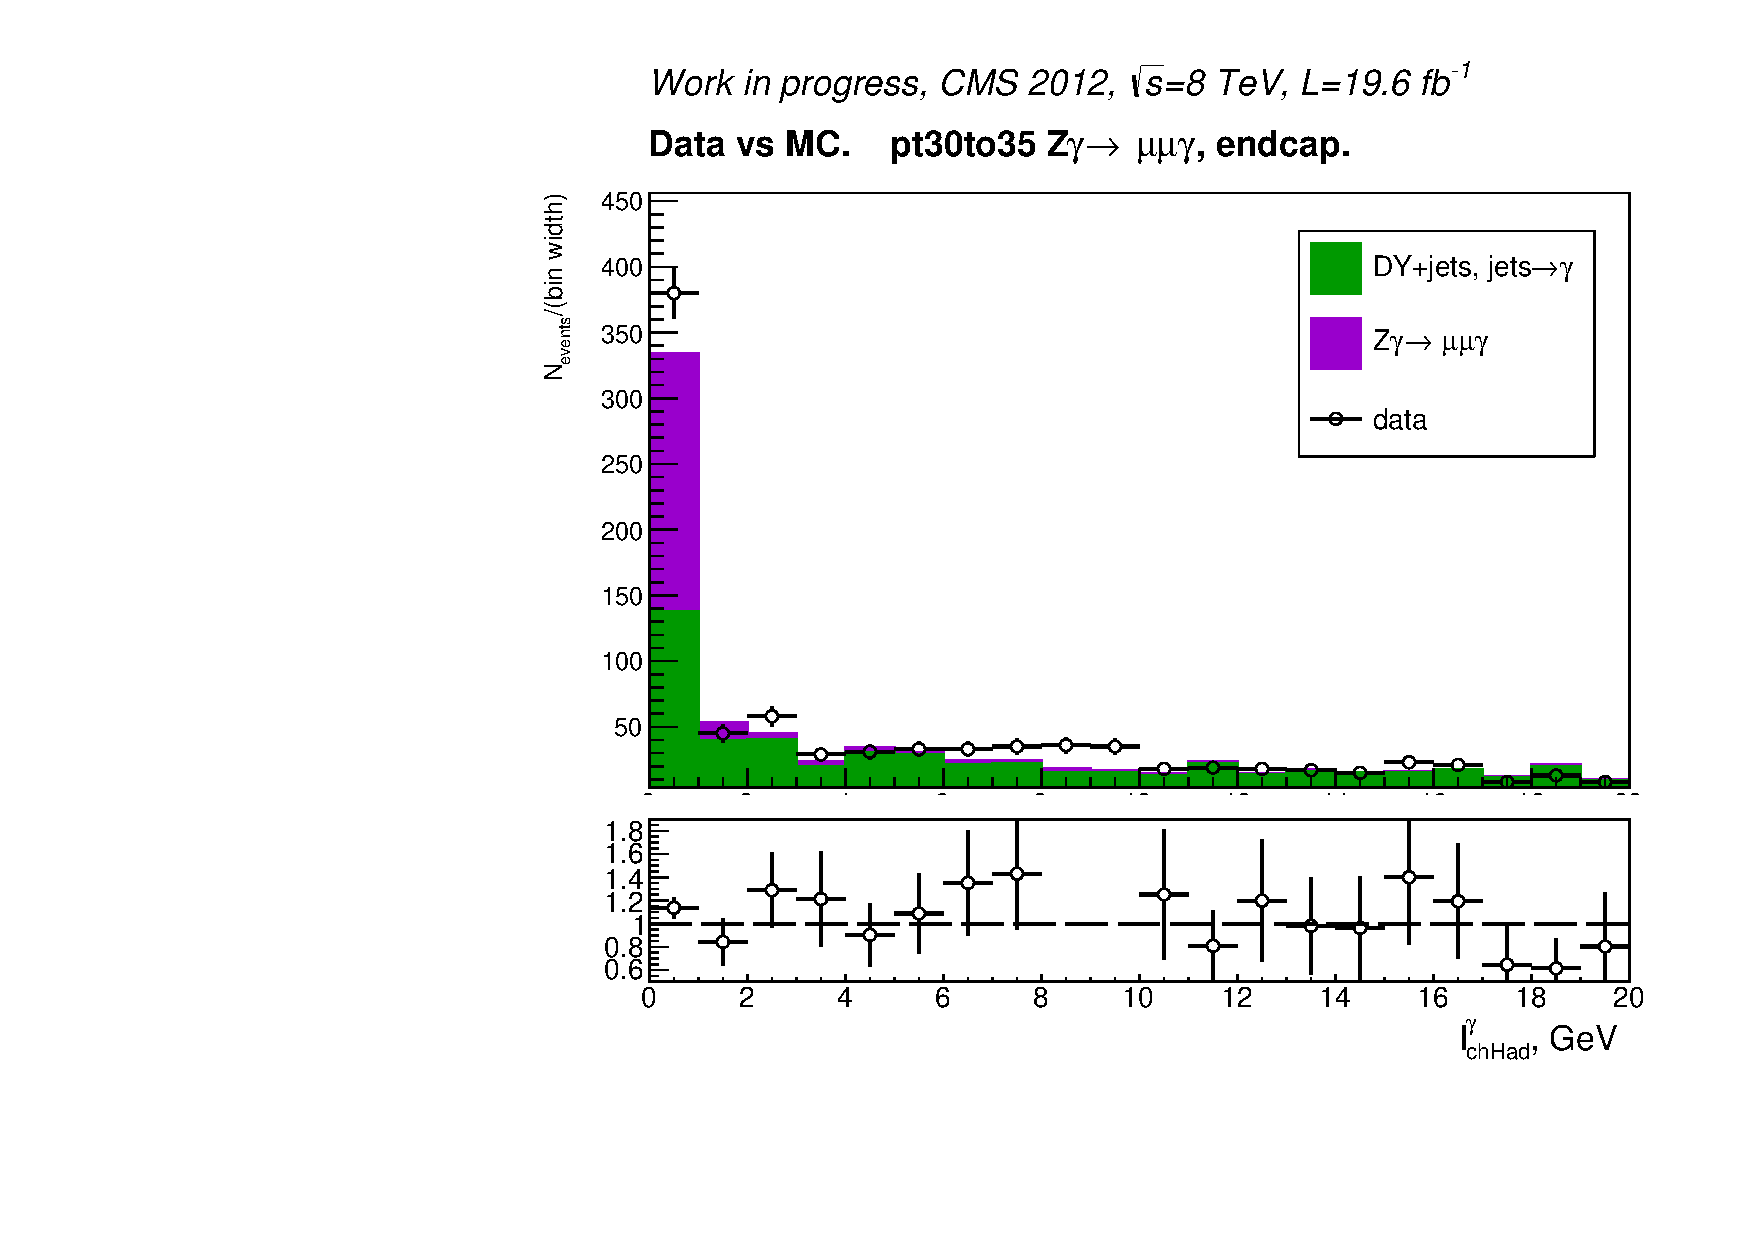
\includegraphics[width=0.32\textwidth]{../figs/figs_v11/MUON_ZGamma/PrepareYields/c_TotalDATAvsMC_Endcap__phoPFChIsoCorrFSR_EXCLUDED_pt30to35_.pdf}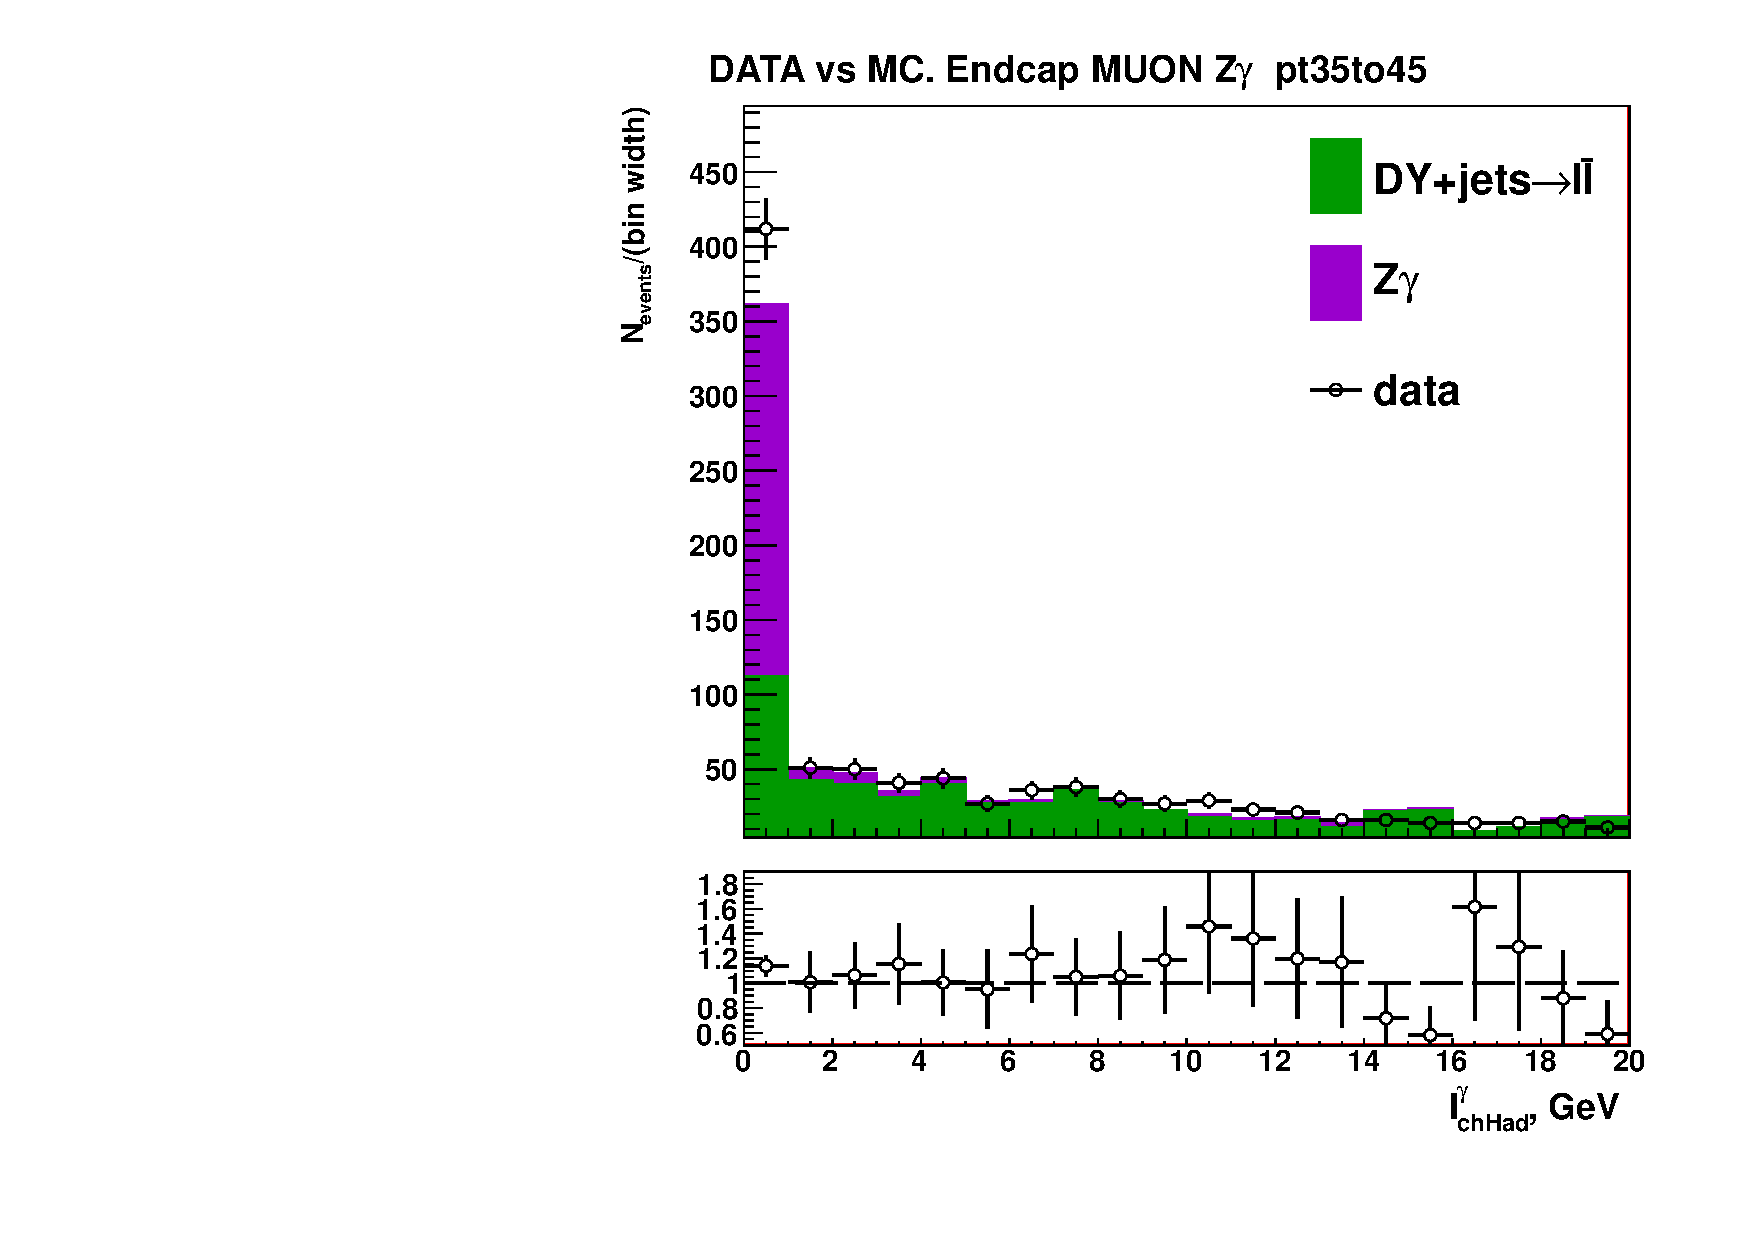
\includegraphics[width=0.32\textwidth]{../figs/figs_v11/MUON_ZGamma/PrepareYields/c_TotalDATAvsMC_Endcap__phoPFChIsoCorrFSR_EXCLUDED_pt35to45_.pdf}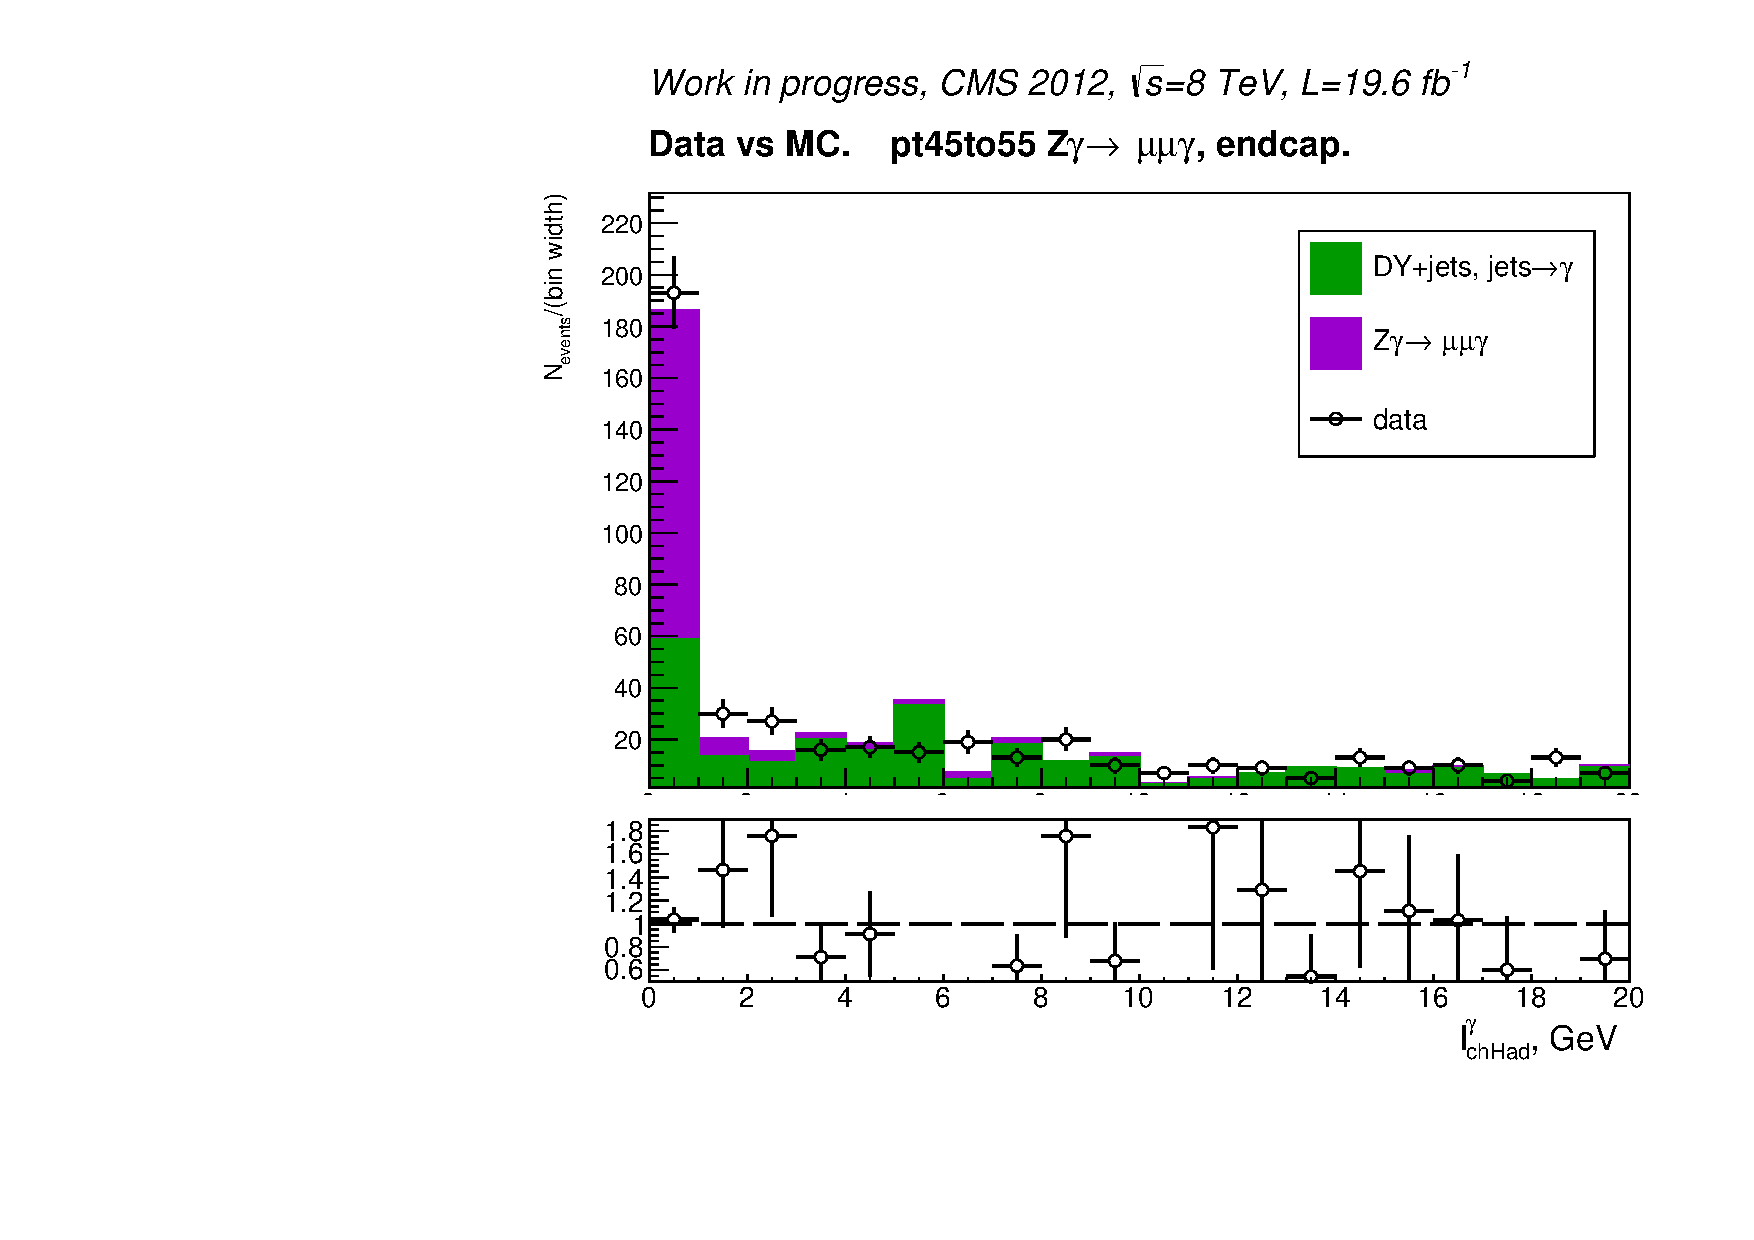
\includegraphics[width=0.32\textwidth]{../figs/figs_v11/MUON_ZGamma/PrepareYields/c_TotalDATAvsMC_Endcap__phoPFChIsoCorrFSR_EXCLUDED_pt45to55_.pdf}\\
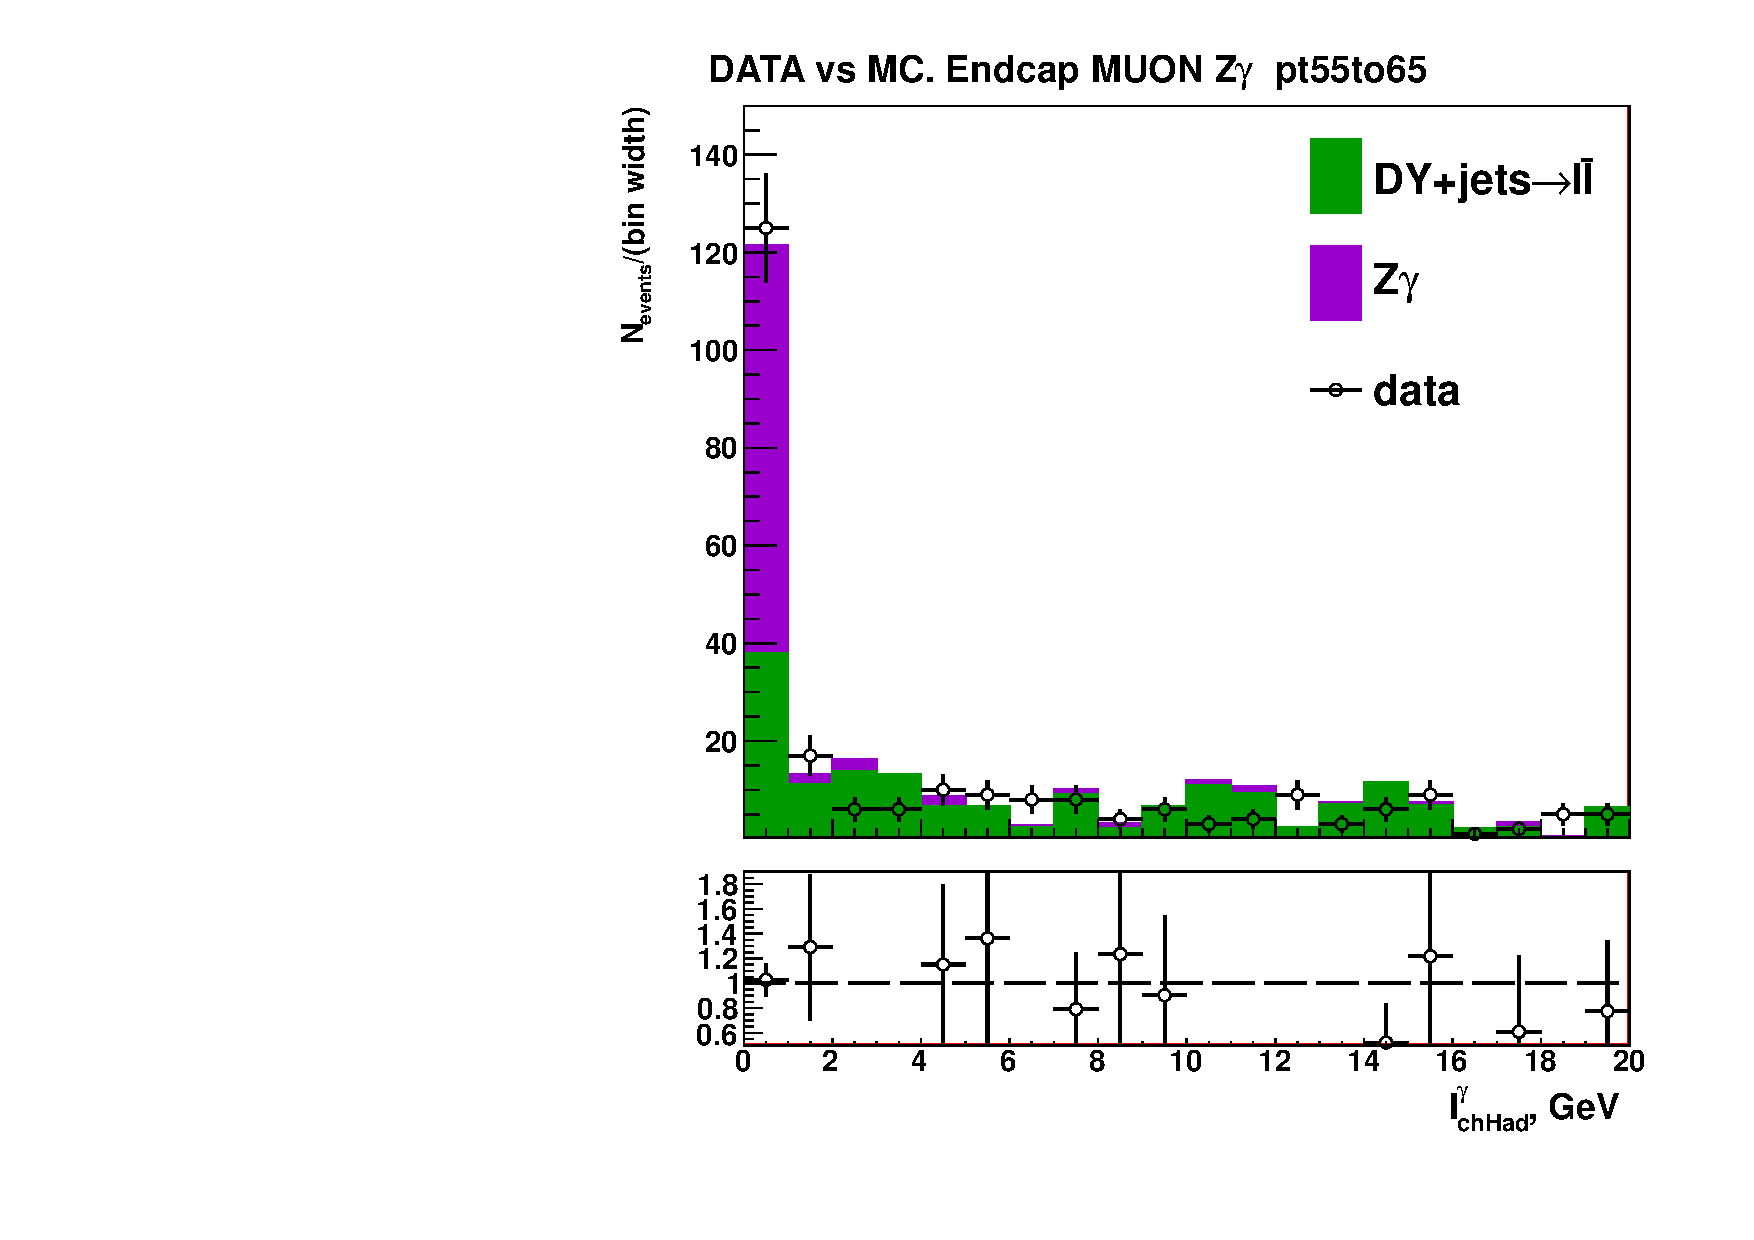
\includegraphics[width=0.32\textwidth]{../figs/figs_v11/MUON_ZGamma/PrepareYields/c_TotalDATAvsMC_Endcap__phoPFChIsoCorrFSR_EXCLUDED_pt55to65_.pdf}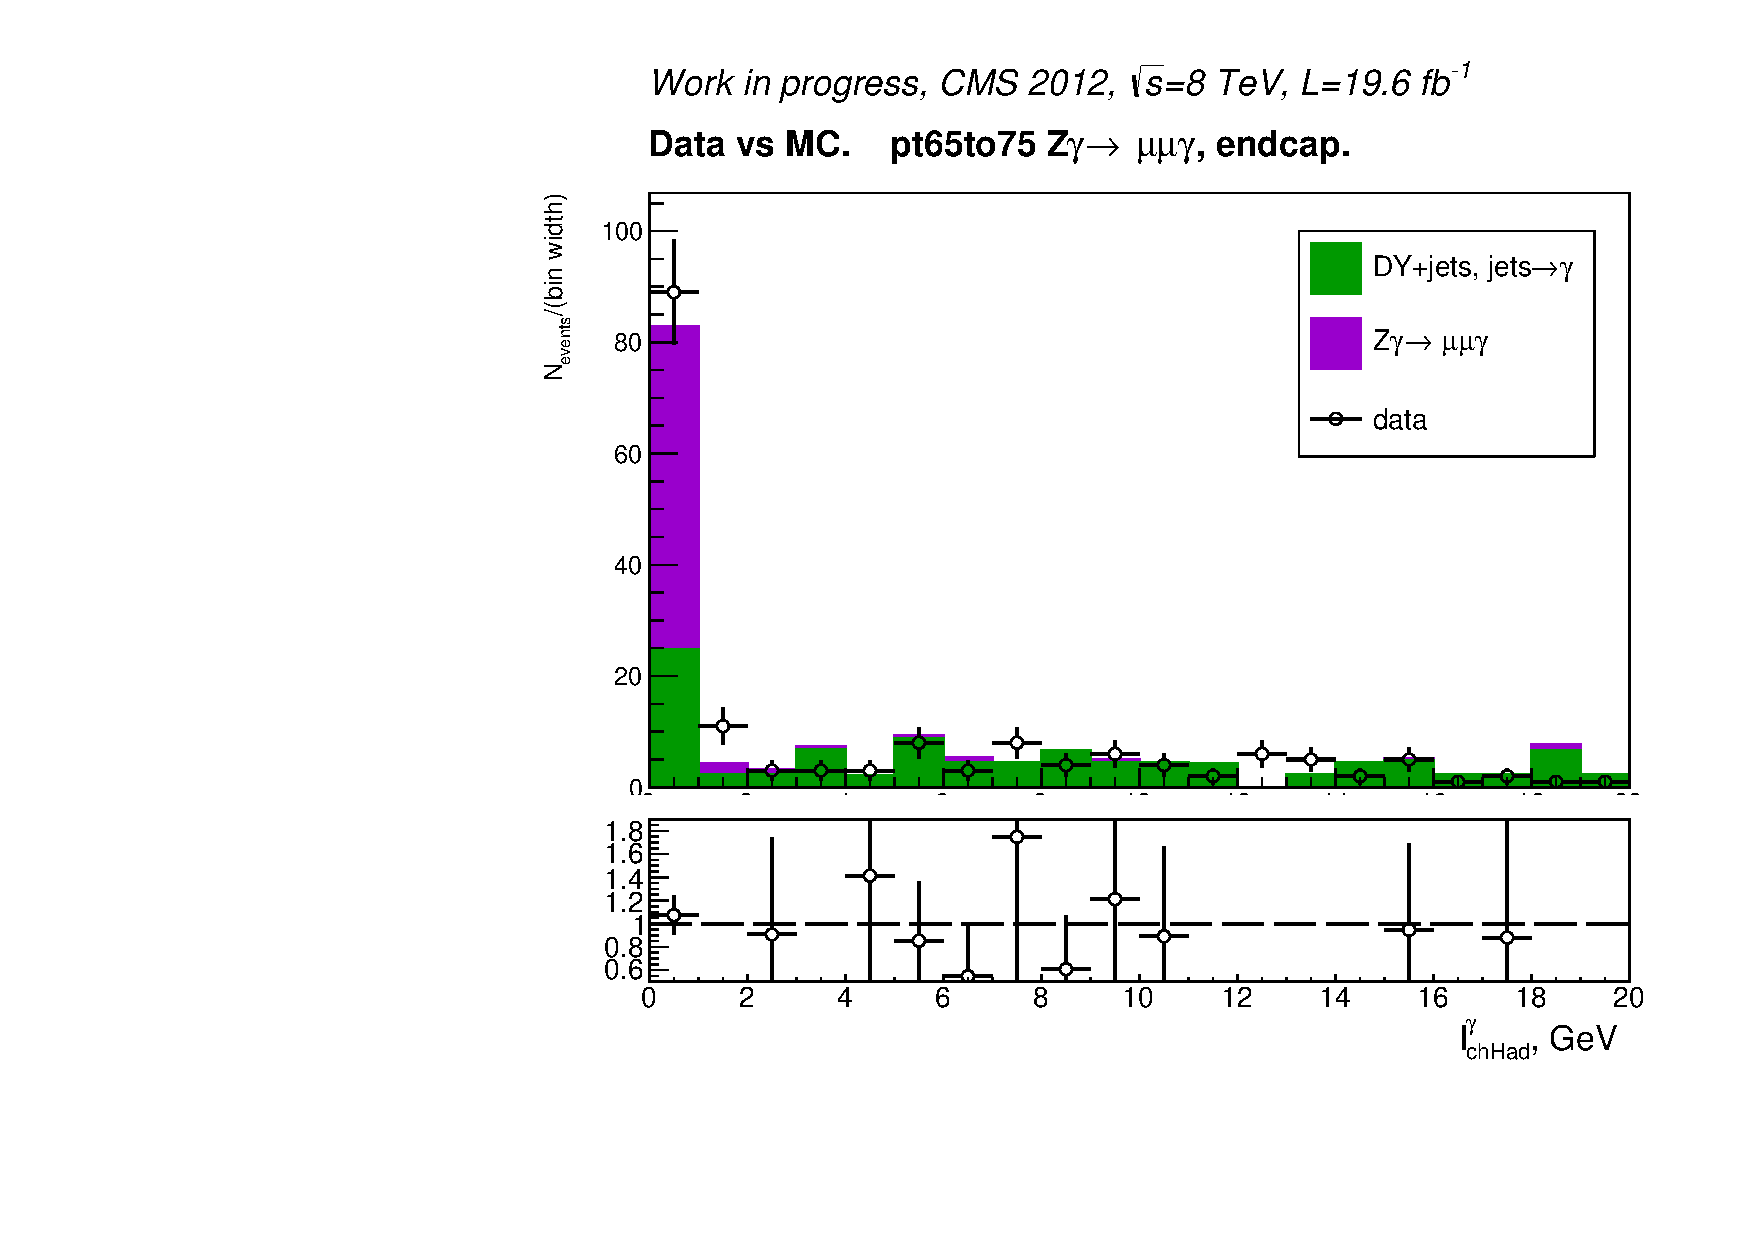
\includegraphics[width=0.32\textwidth]{../figs/figs_v11/MUON_ZGamma/PrepareYields/c_TotalDATAvsMC_Endcap__phoPFChIsoCorrFSR_EXCLUDED_pt65to75_.pdf}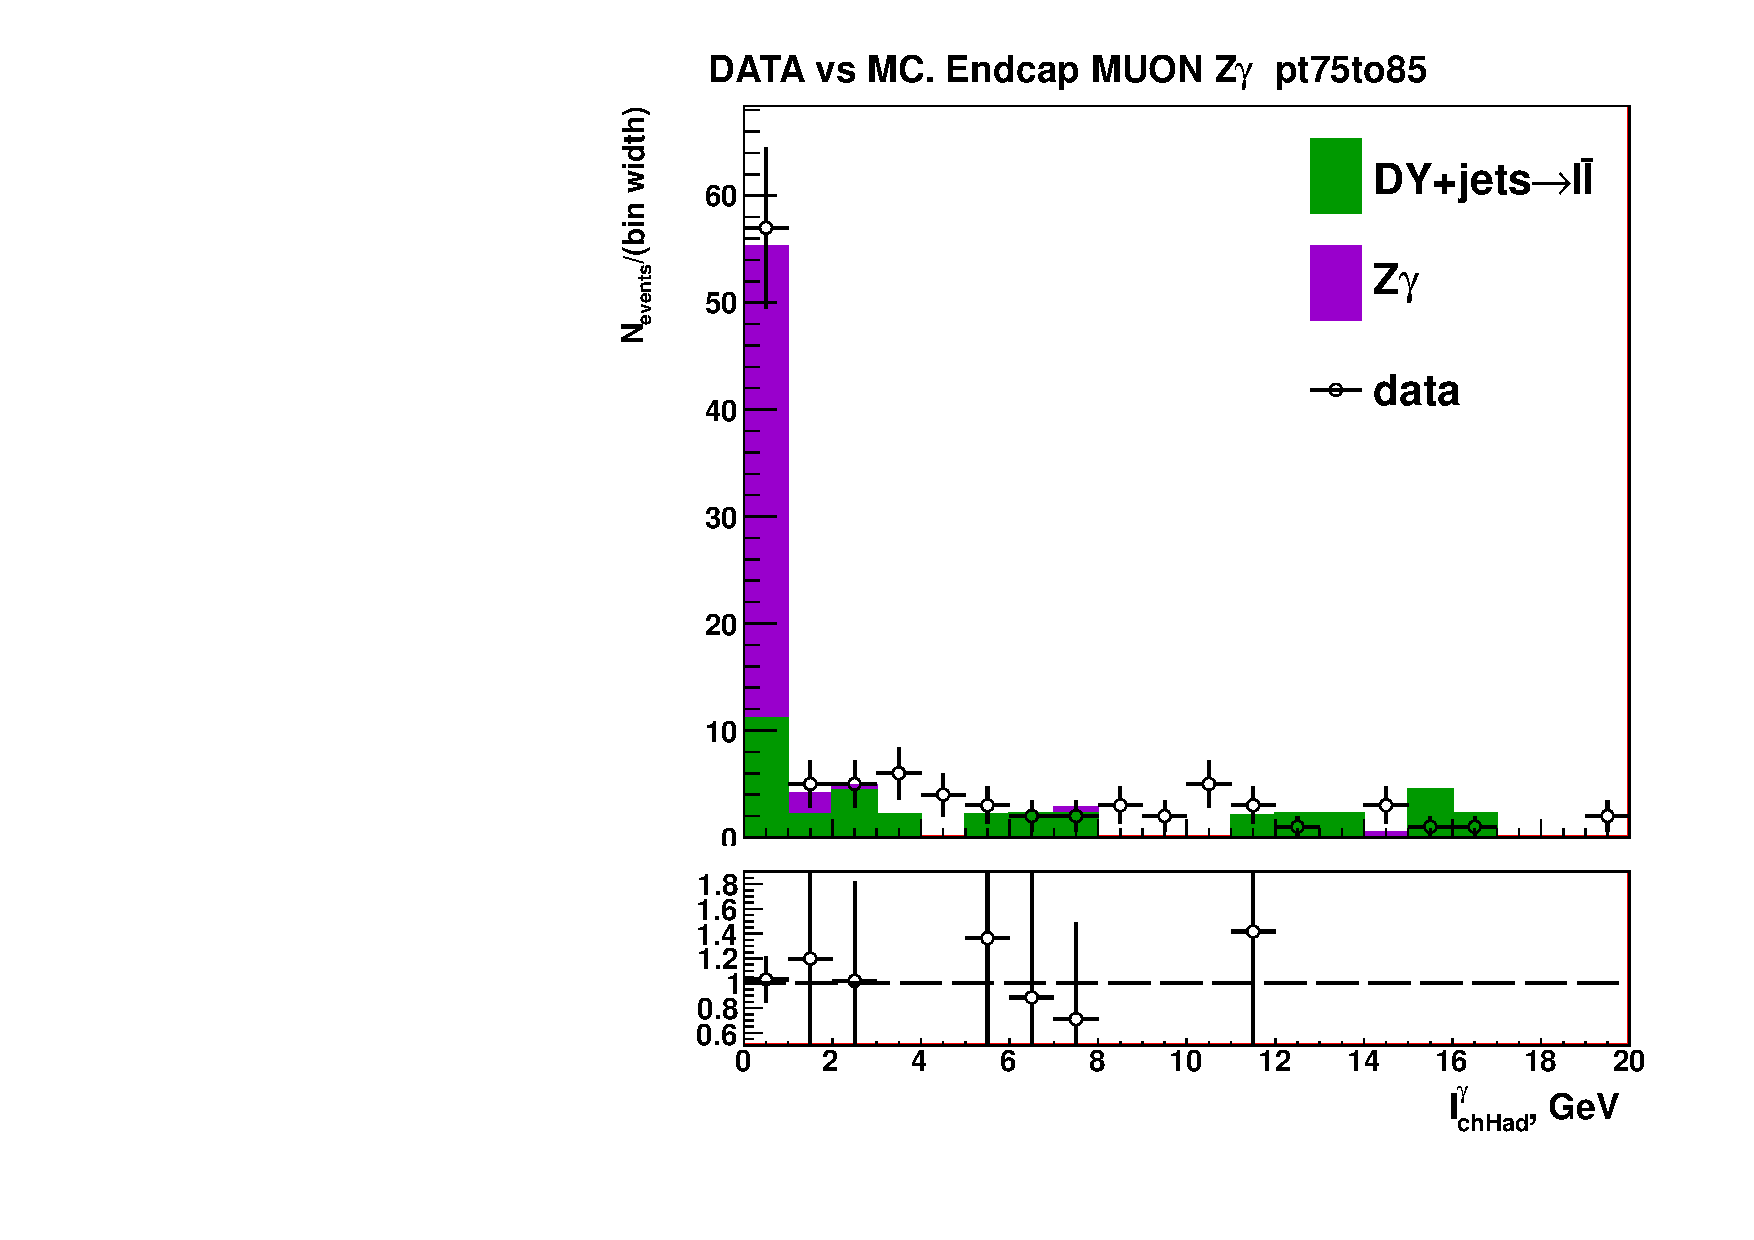
\includegraphics[width=0.32\textwidth]{../figs/figs_v11/MUON_ZGamma/PrepareYields/c_TotalDATAvsMC_Endcap__phoPFChIsoCorrFSR_EXCLUDED_pt75to85_.pdf}\\
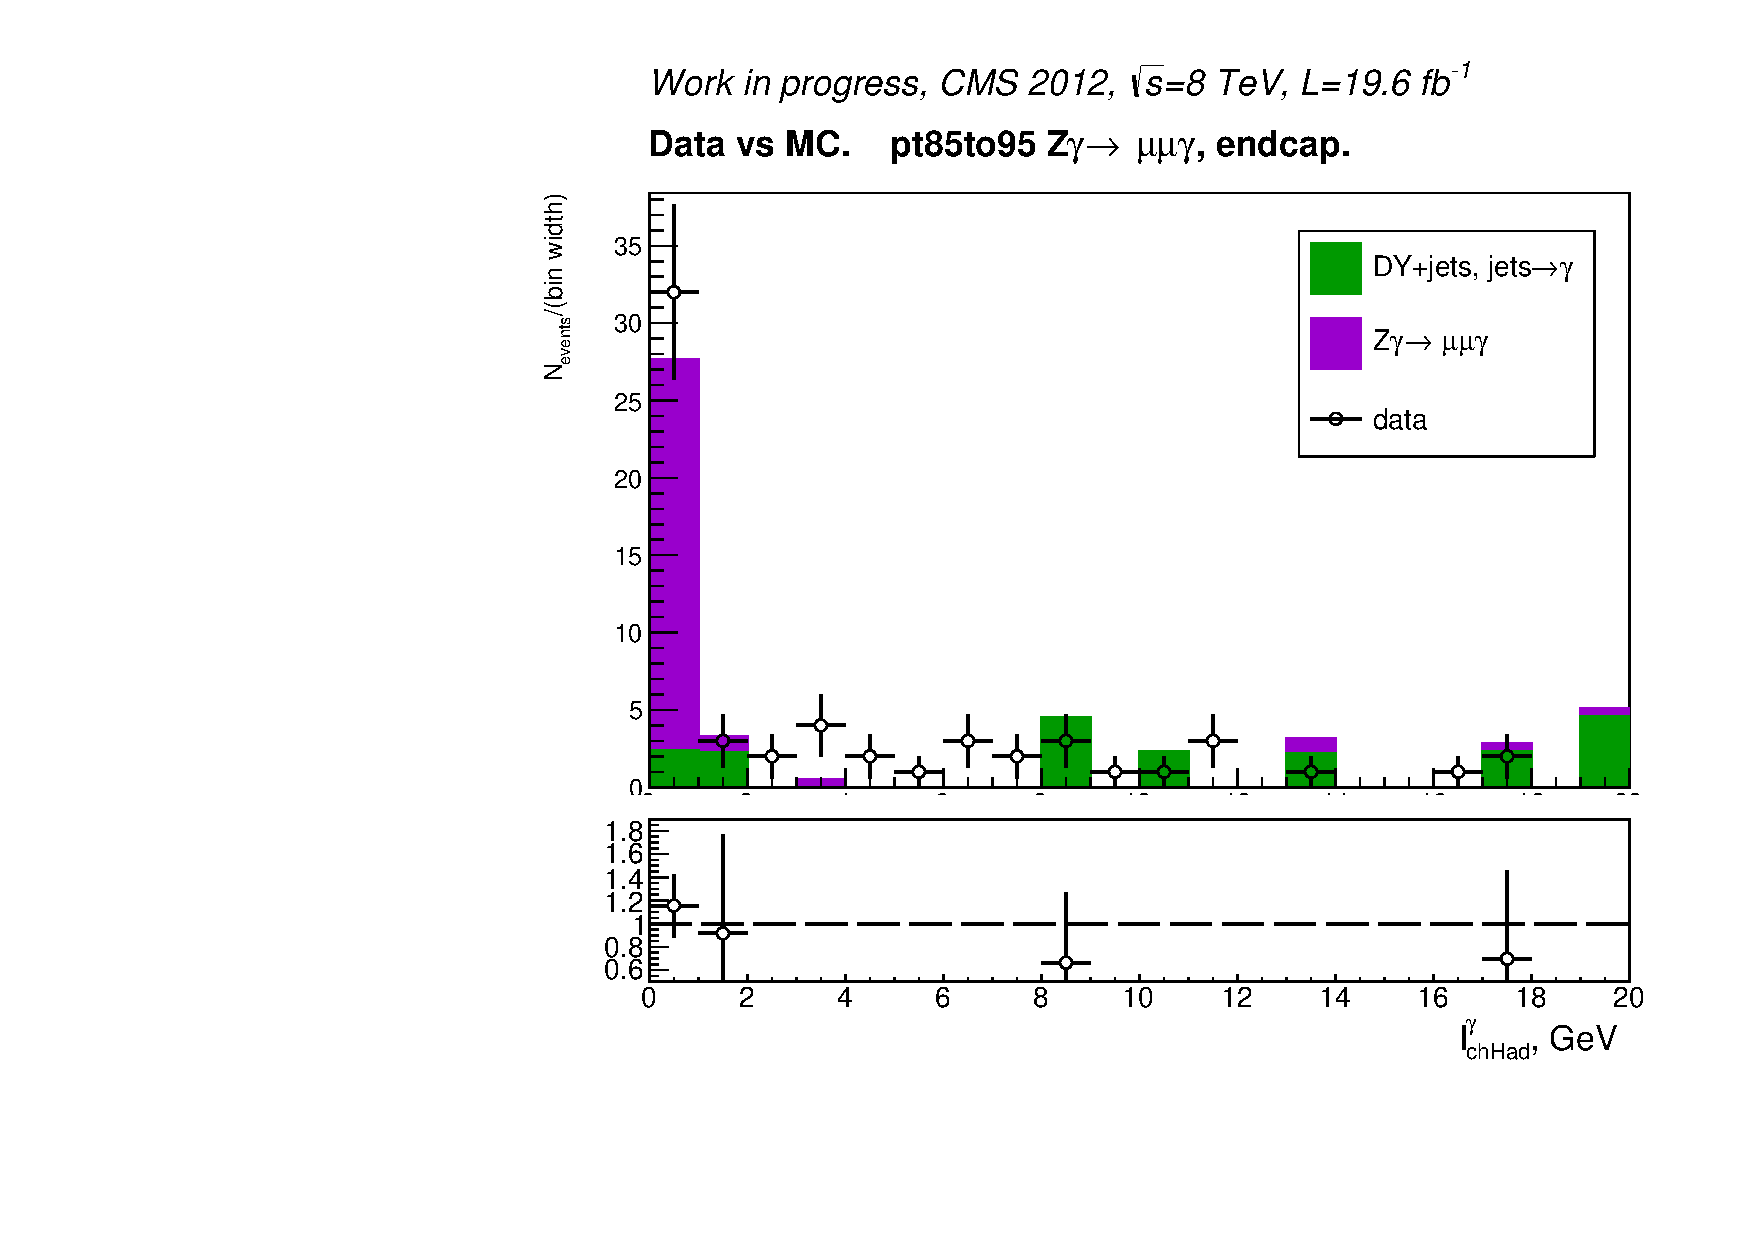
\includegraphics[width=0.32\textwidth]{../figs/figs_v11/MUON_ZGamma/PrepareYields/c_TotalDATAvsMC_Endcap__phoPFChIsoCorrFSR_EXCLUDED_pt85to95_.pdf}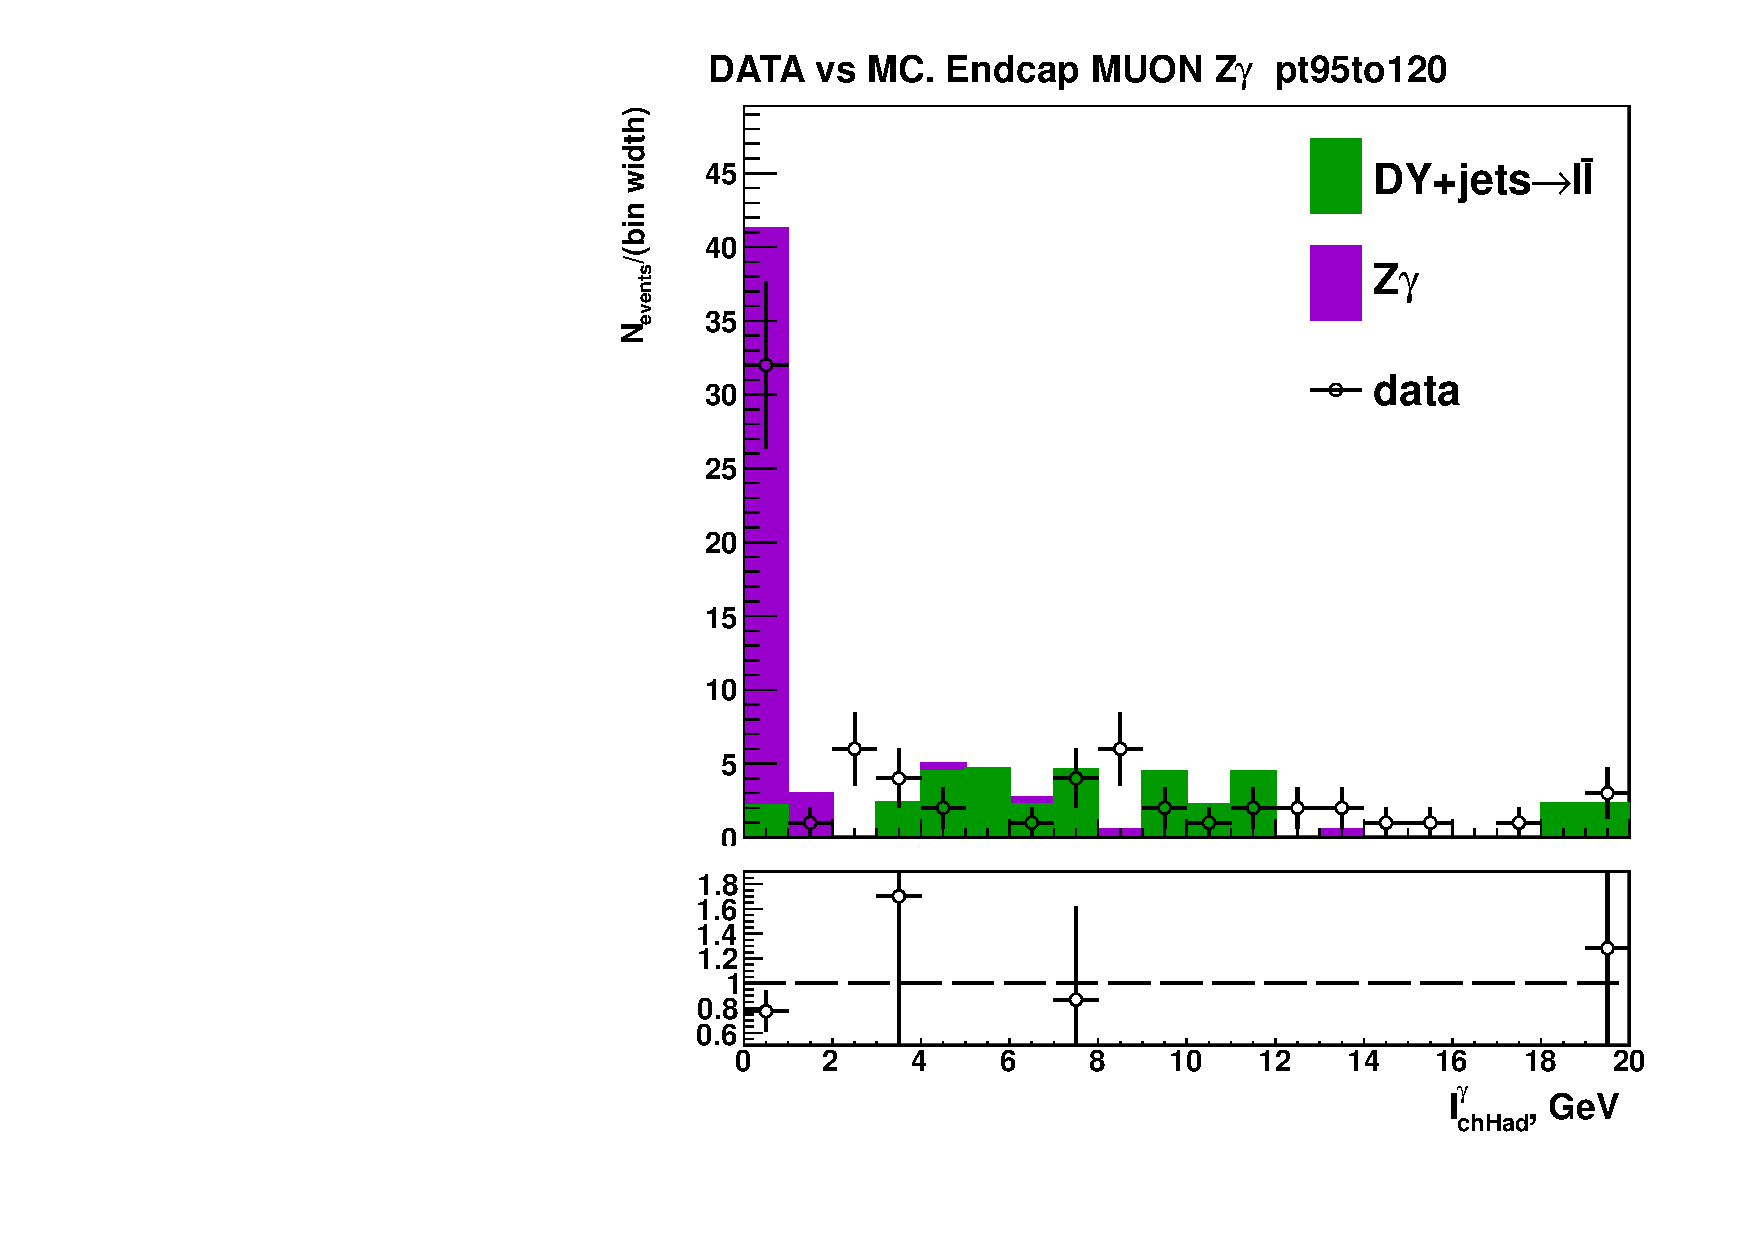
\includegraphics[width=0.32\textwidth]{../figs/figs_v11/MUON_ZGamma/PrepareYields/c_TotalDATAvsMC_Endcap__phoPFChIsoCorrFSR_EXCLUDED_pt95to120_.pdf}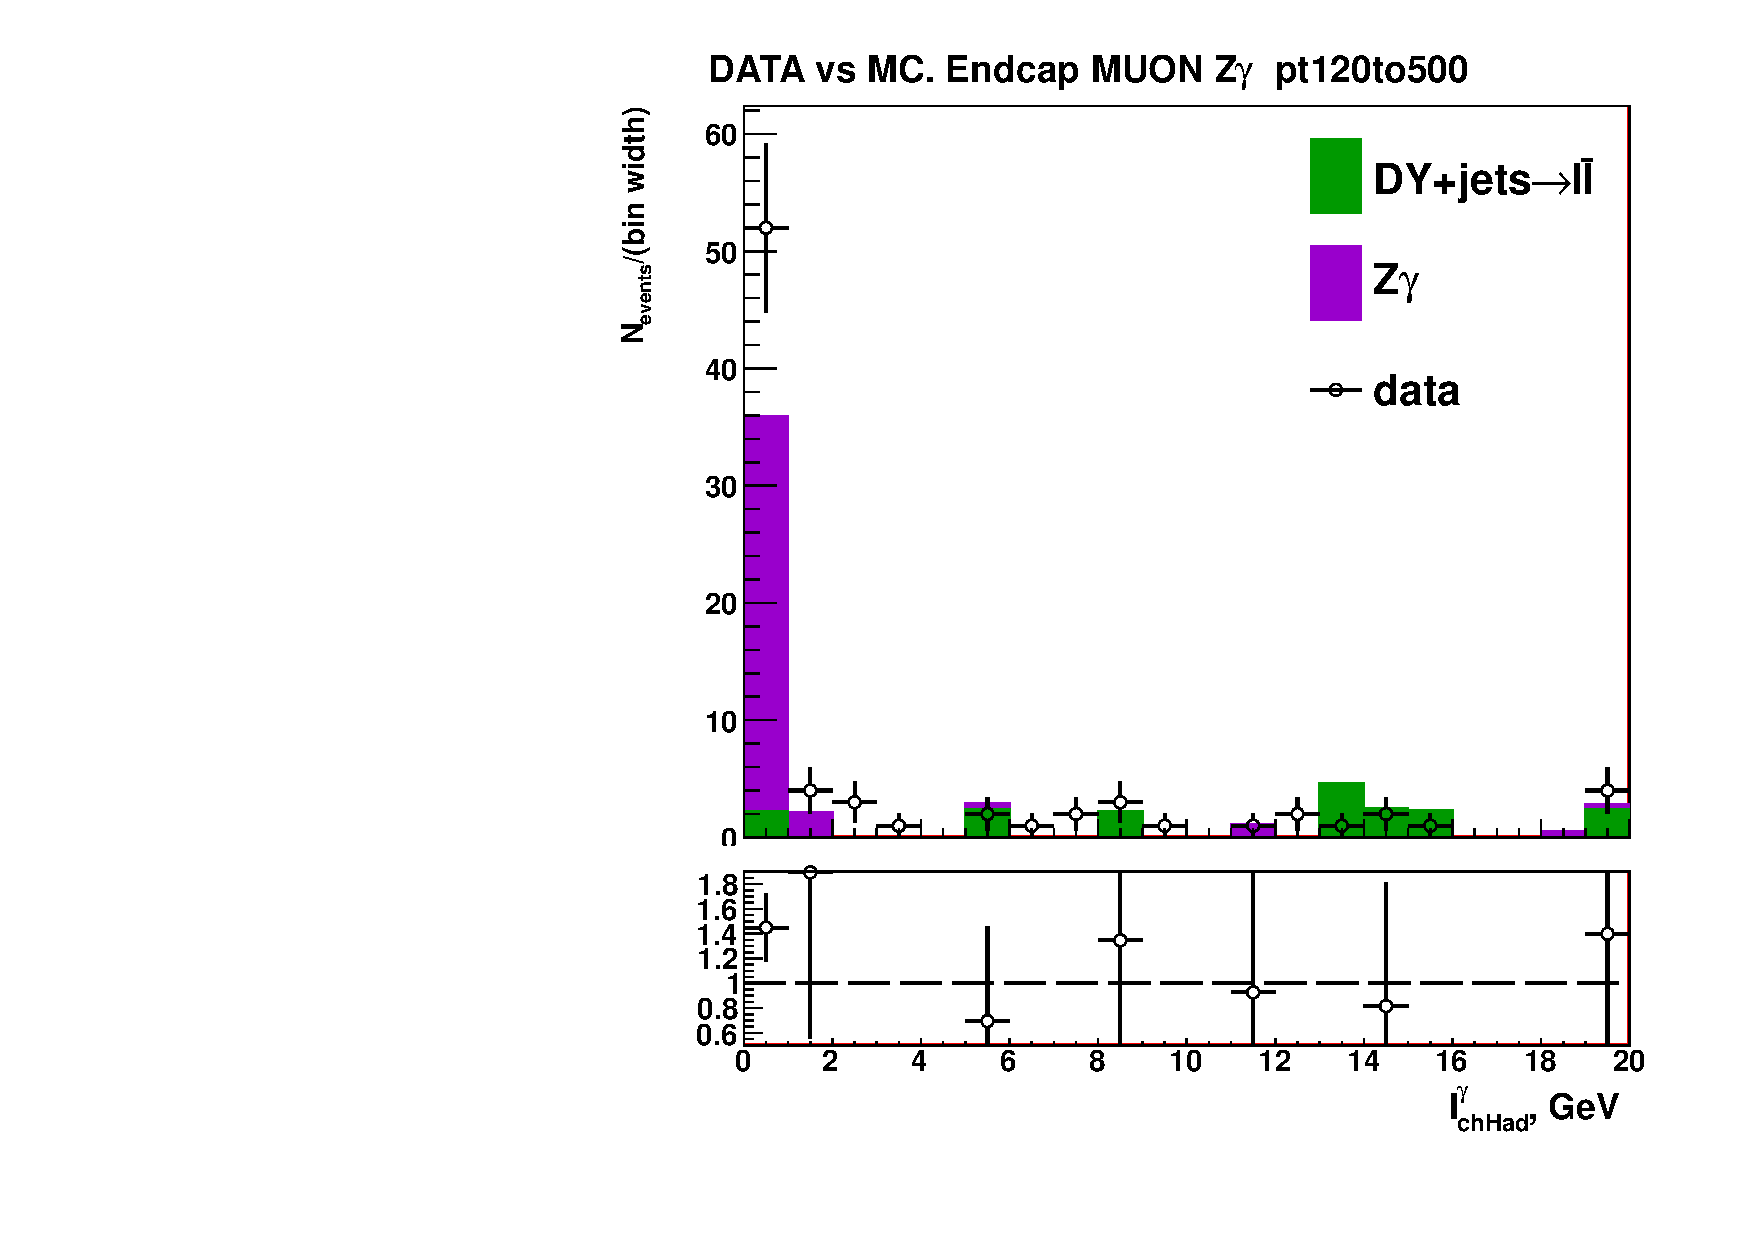
\includegraphics[width=0.32\textwidth]{../figs/figs_v11/MUON_ZGamma/PrepareYields/c_TotalDATAvsMC_Endcap__phoPFChIsoCorrFSR_EXCLUDED_pt120to500_.pdf}\\
  \caption{$Z\gamma$-selected ISR events, data vs MC. Distributions of $I_{chHad}^{\gamma}$ used for preparing fake-$\gamma$ templates. Real-$\gamma$ contribution to ISR region is subtracted based on $Z\gamma$ signal MC prediction to prepare fake-$\gamma$ templates. Ranges of $P_T^{\gamma}$ are shown in the plot titles and cover the total range of 15~GeV$<P_T^{\gamma}<$500~GeV. EE photons.}
  \label{fig:Zg_ISR_phoPFChIsoCorr_Endcap}
  \end{center}
\end{figure}

\begin{figure}[htb]
  \begin{center}
   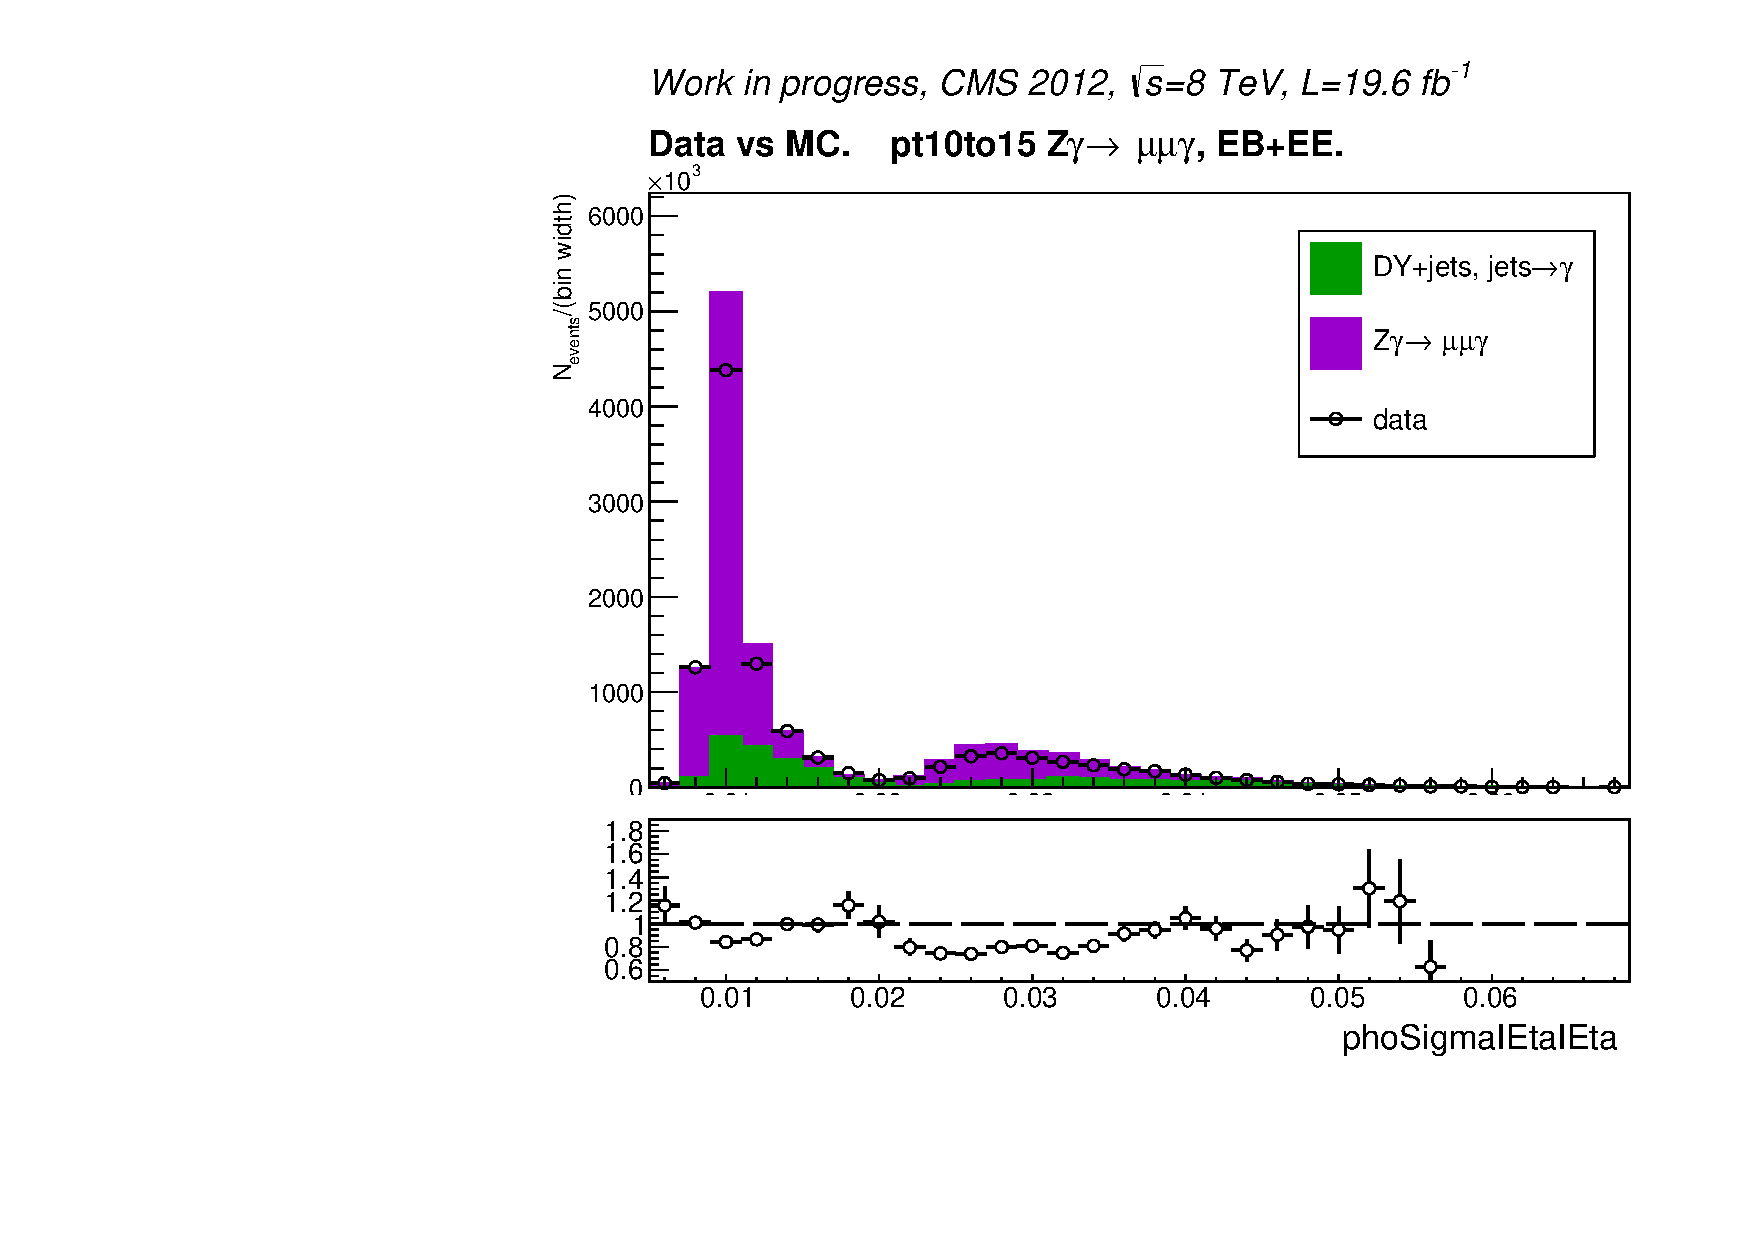
\includegraphics[width=0.45\textwidth]{../figs/figs_v11/MUON_ZGamma/PrepareYields/c_TotalDATAvsMC_EtaCommon__phoSigmaIEtaIEtaFSR_pt10to15_.pdf}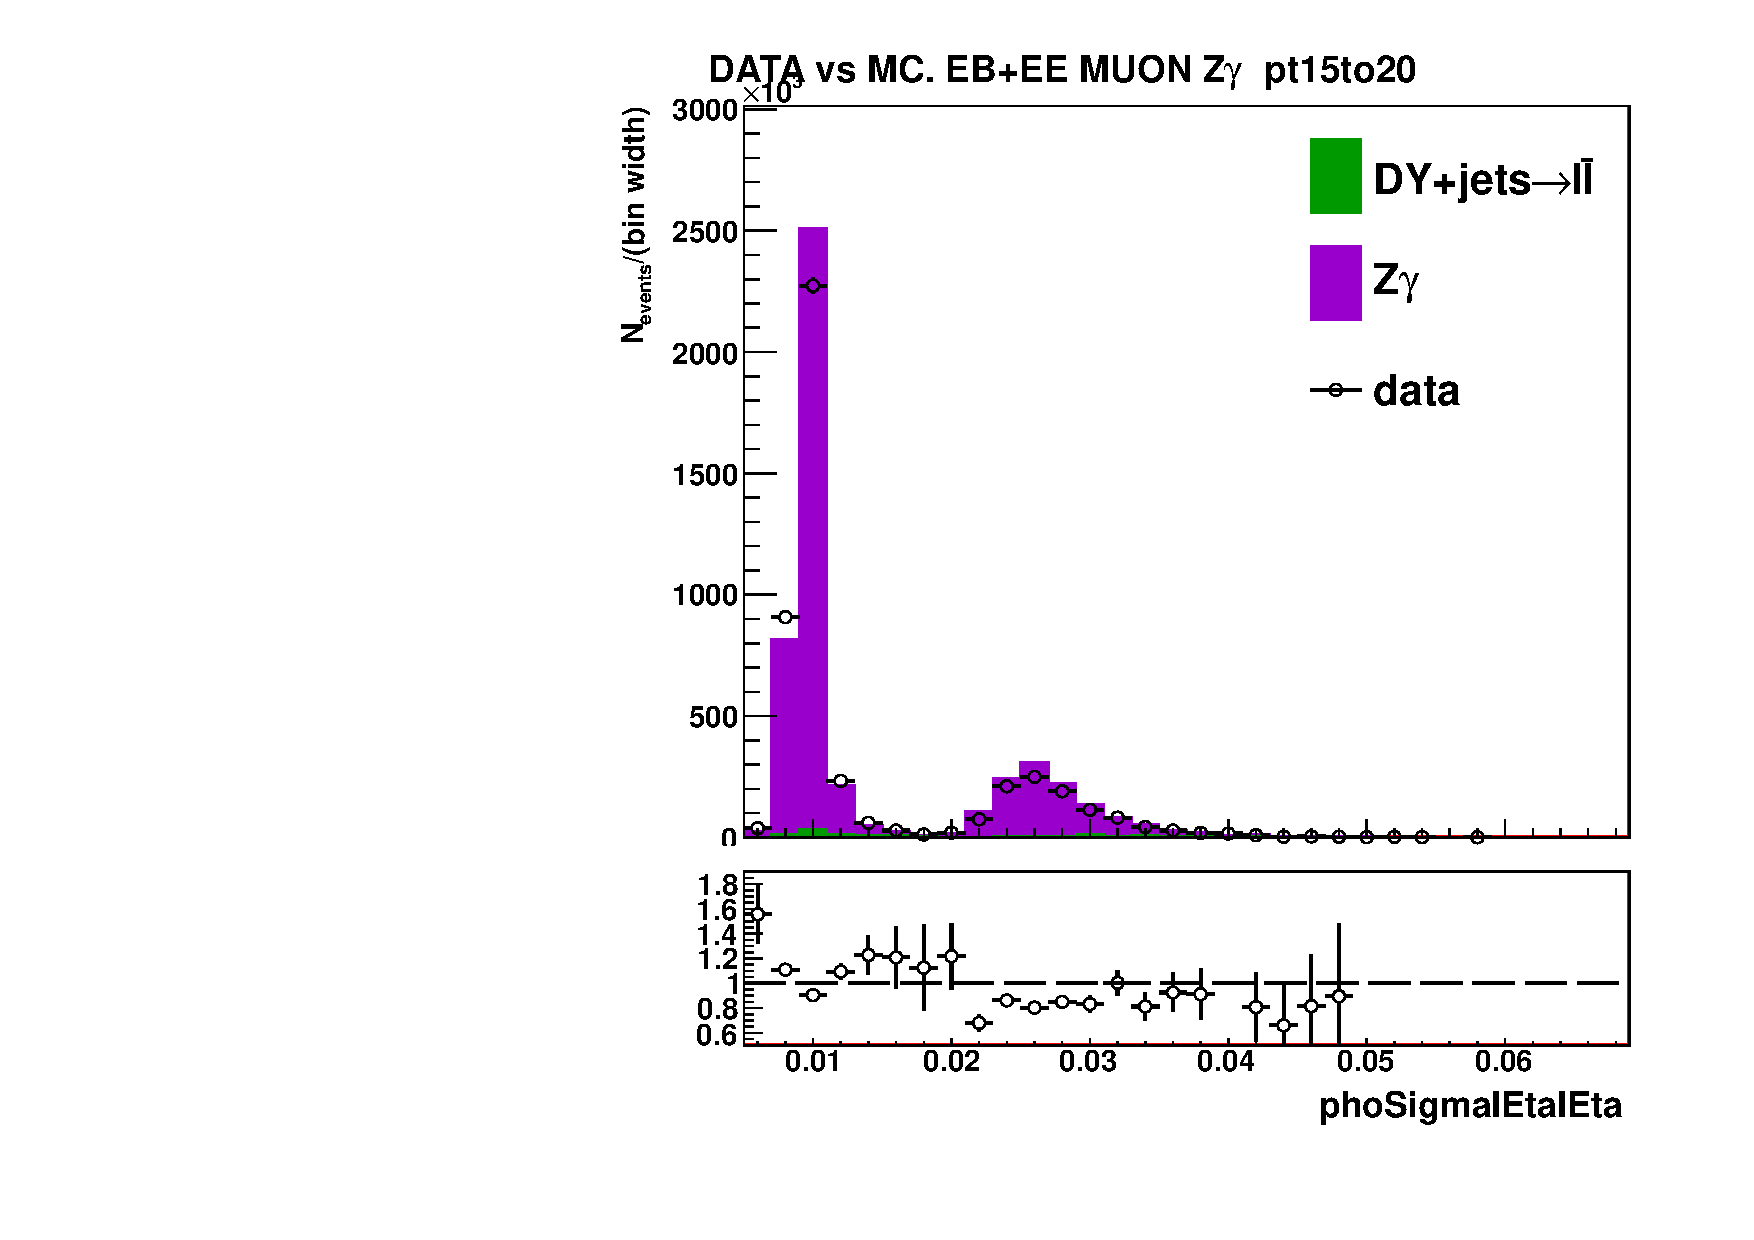
\includegraphics[width=0.45\textwidth]{../figs/figs_v11/MUON_ZGamma/PrepareYields/c_TotalDATAvsMC_EtaCommon__phoSigmaIEtaIEtaFSR_pt15to20_.pdf}\\
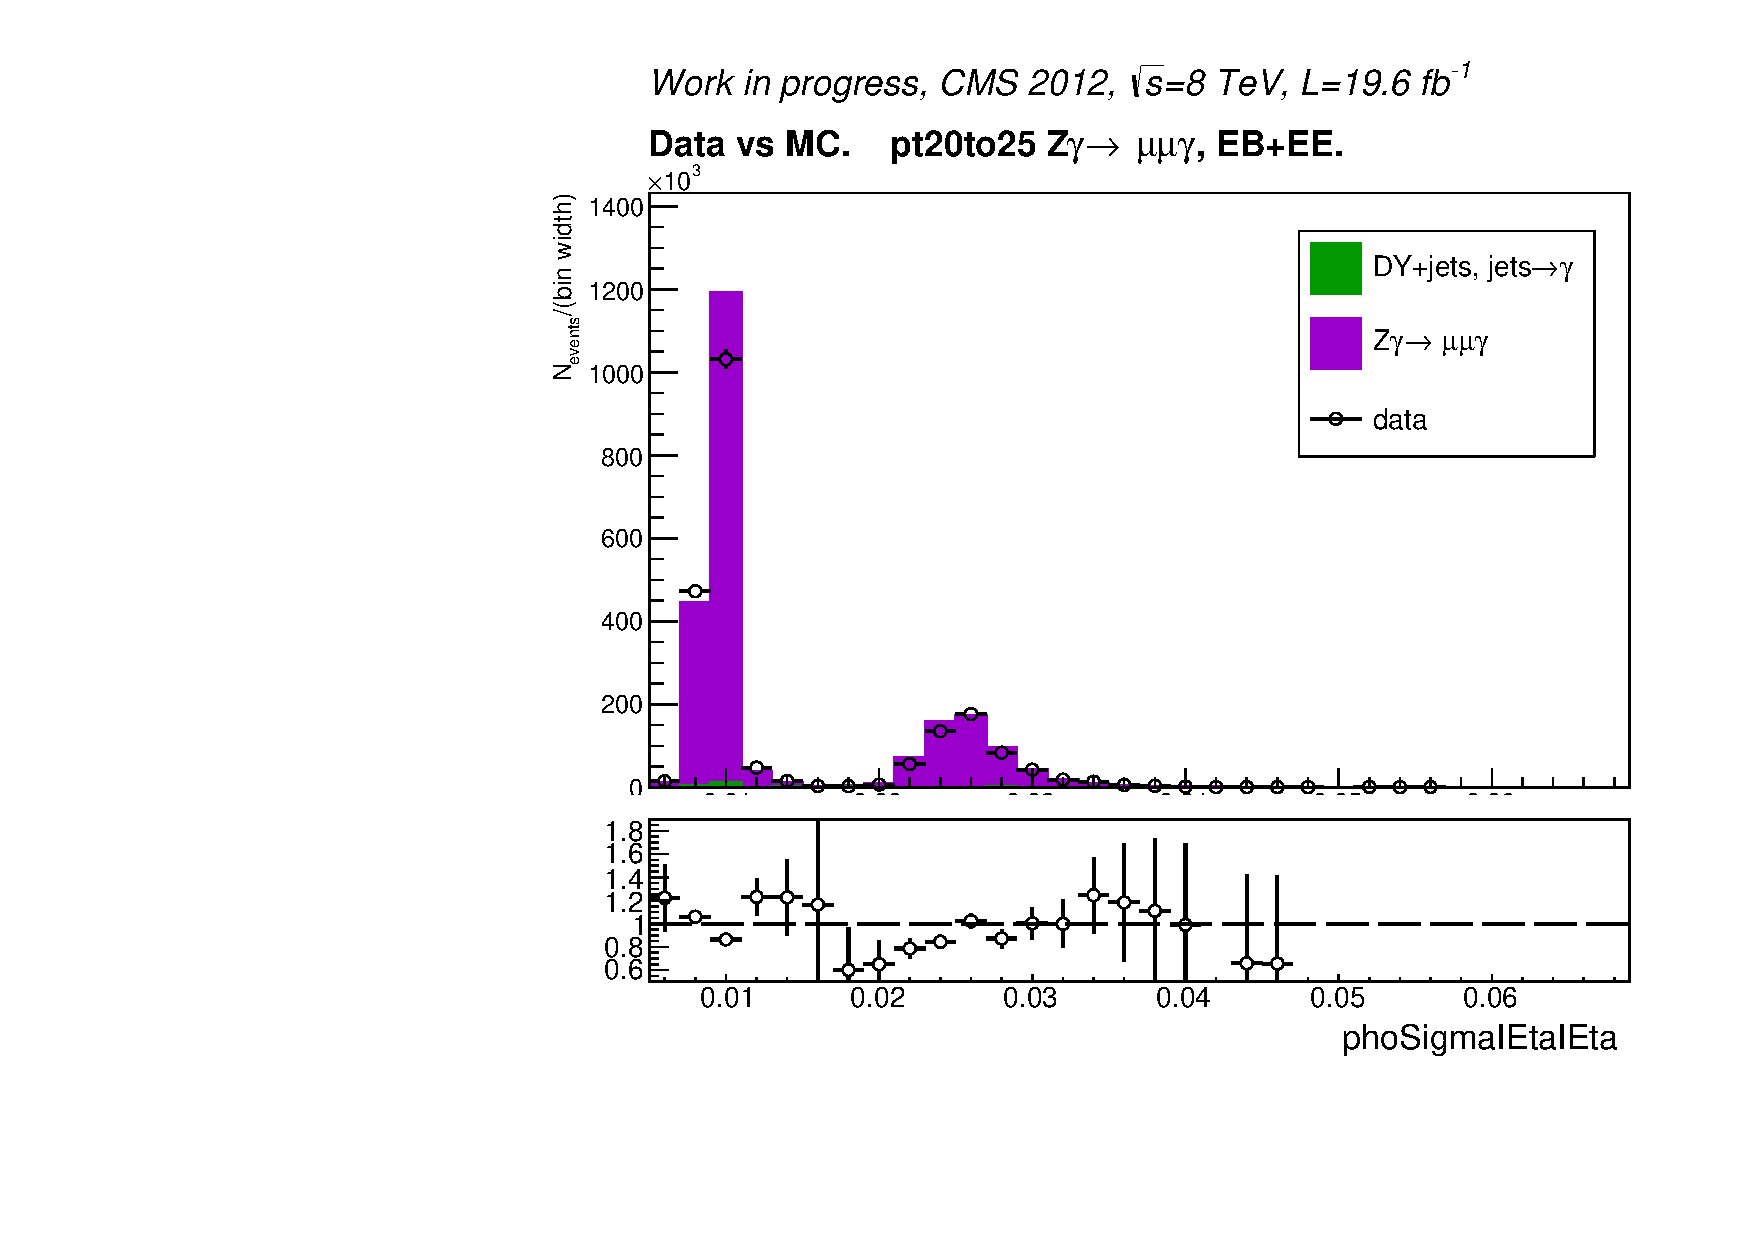
\includegraphics[width=0.32\textwidth]{../figs/figs_v11/MUON_ZGamma/PrepareYields/c_TotalDATAvsMC_EtaCommon__phoSigmaIEtaIEtaFSR_pt20to25_.pdf}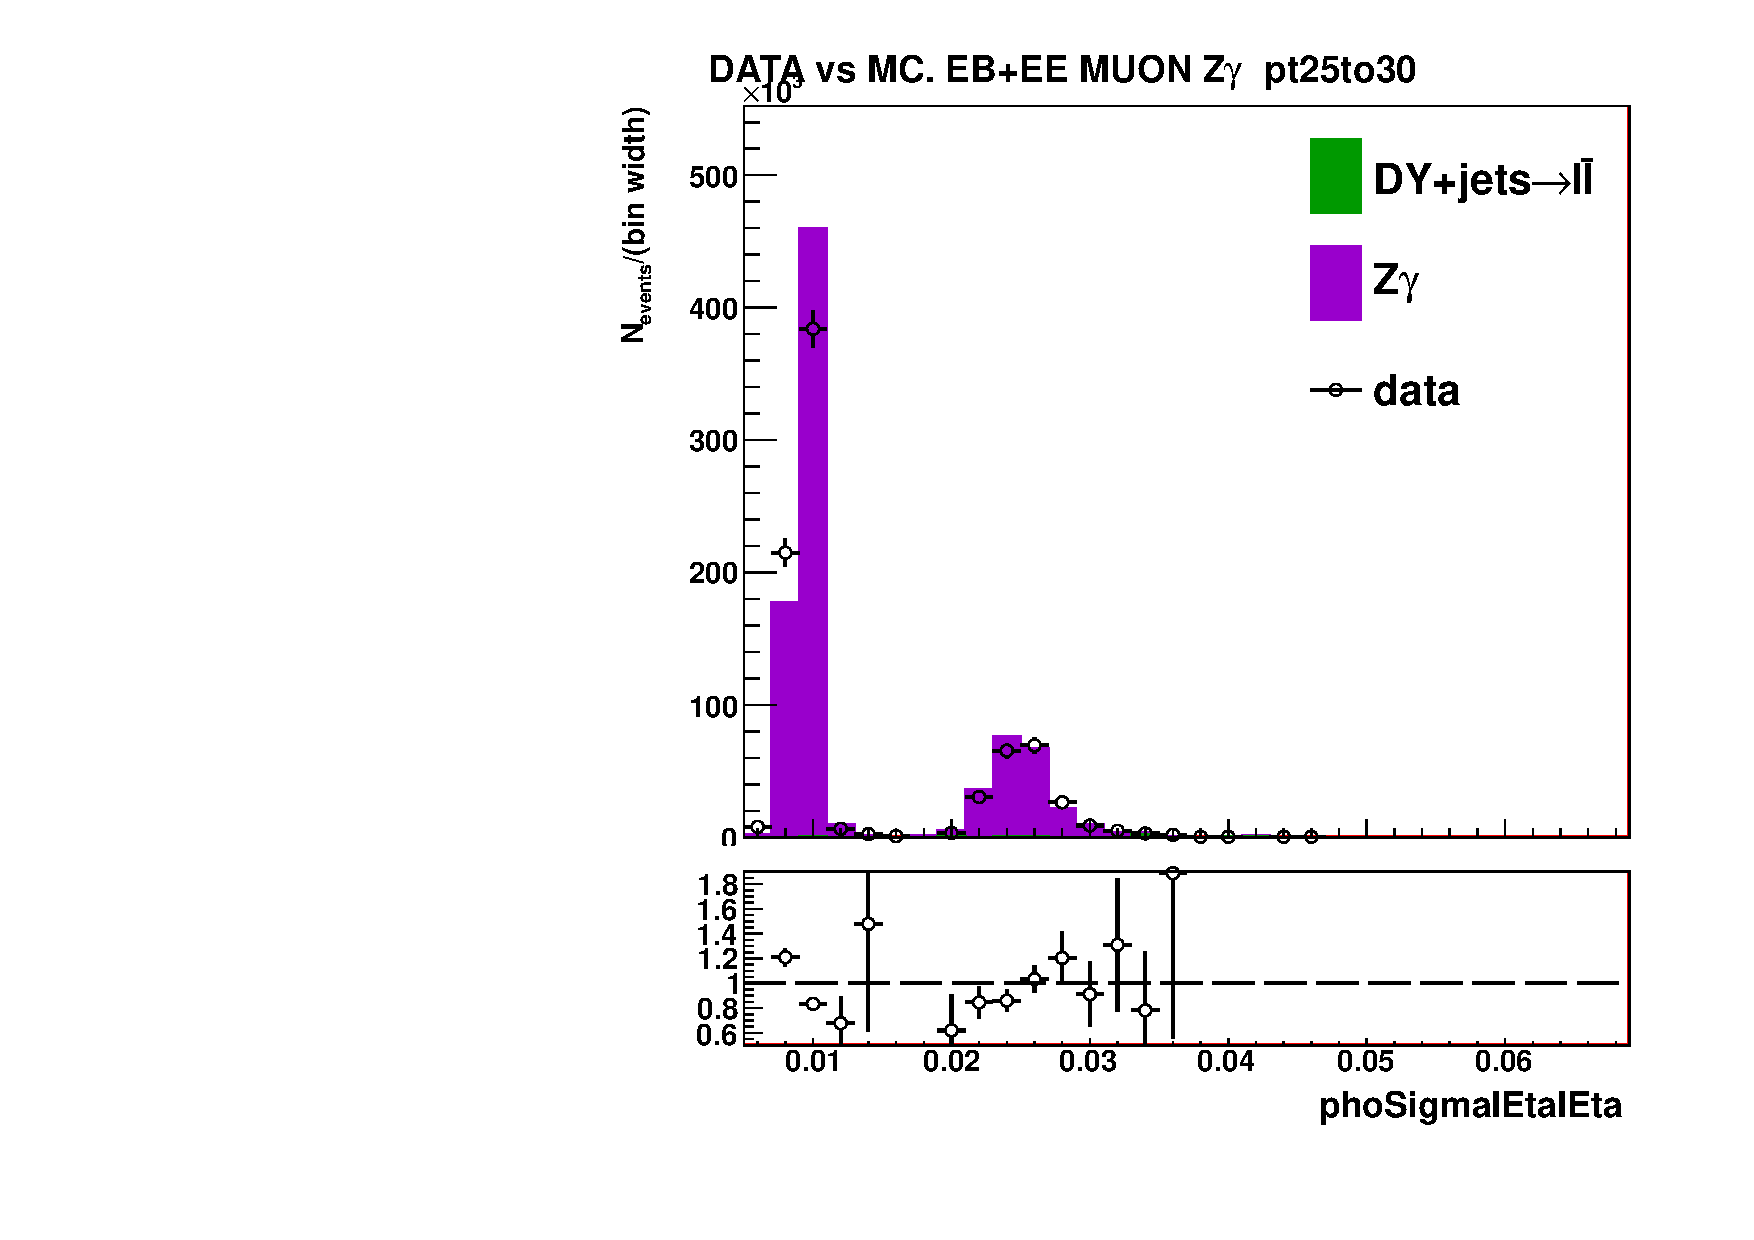
\includegraphics[width=0.32\textwidth]{../figs/figs_v11/MUON_ZGamma/PrepareYields/c_TotalDATAvsMC_EtaCommon__phoSigmaIEtaIEtaFSR_pt25to30_.pdf}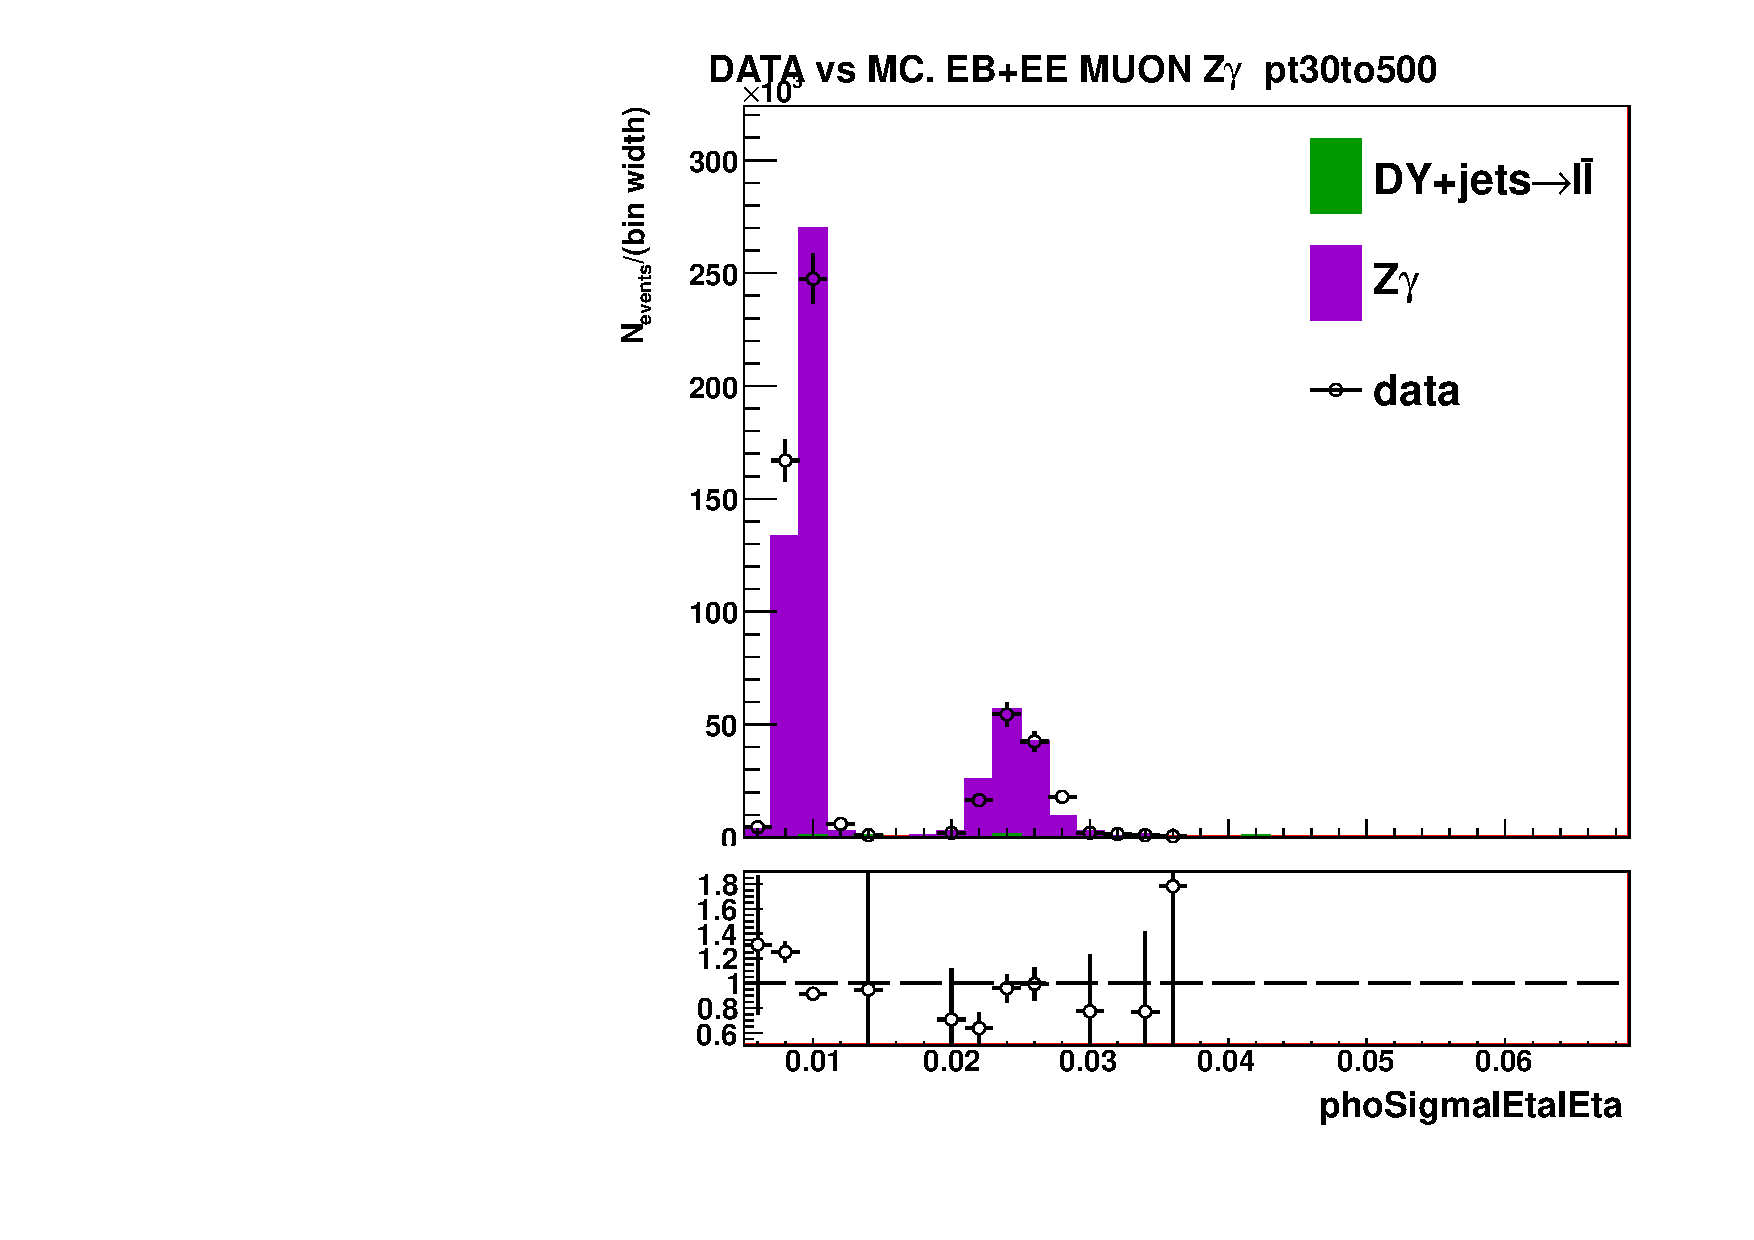
\includegraphics[width=0.32\textwidth]{../figs/figs_v11/MUON_ZGamma/PrepareYields/c_TotalDATAvsMC_EtaCommon__phoSigmaIEtaIEtaFSR_pt30to500_.pdf}\\
  \caption{$Z\gamma$-selected FSR events, data vs MC. Distributions of $\sigma_{i\eta i \eta}$ are used for preparing real-$\gamma$ templates. Fake-$\gamma$ contribution to FSR region is subtracted based on DY+jets MC prediction to prepare real-$\gamma$ templates. The templates are prepared separately for barrel and endcap photons.}
  \label{fig:Zg_FSR_phoSigmaIEtaIEta}
  \end{center}
\end{figure}

\begin{figure}[htb]
  \begin{center}
   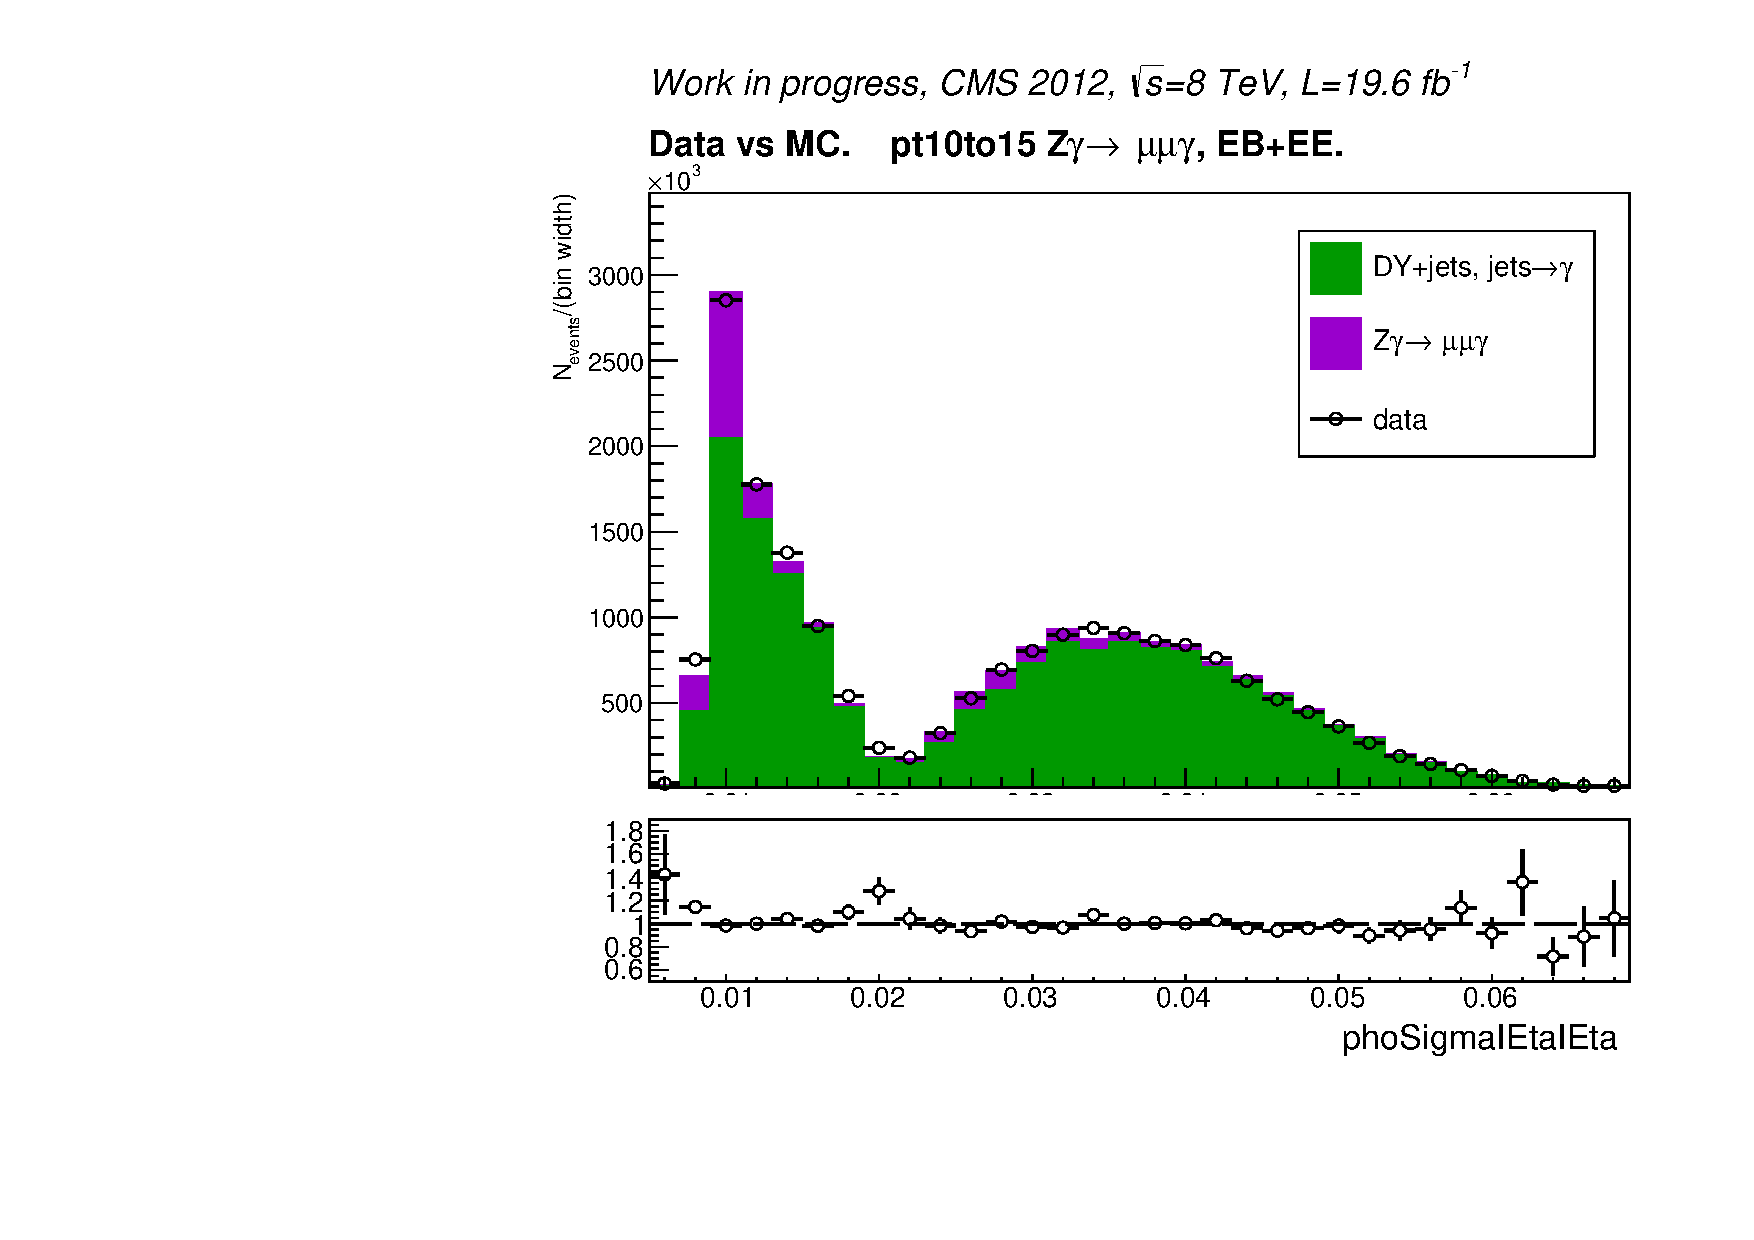
\includegraphics[width=0.45\textwidth]{../figs/figs_v11/MUON_ZGamma/PrepareYields/c_TotalDATAvsMC_EtaCommon__phoSigmaIEtaIEtaFSR_EXCLUDED_pt10to15_.pdf}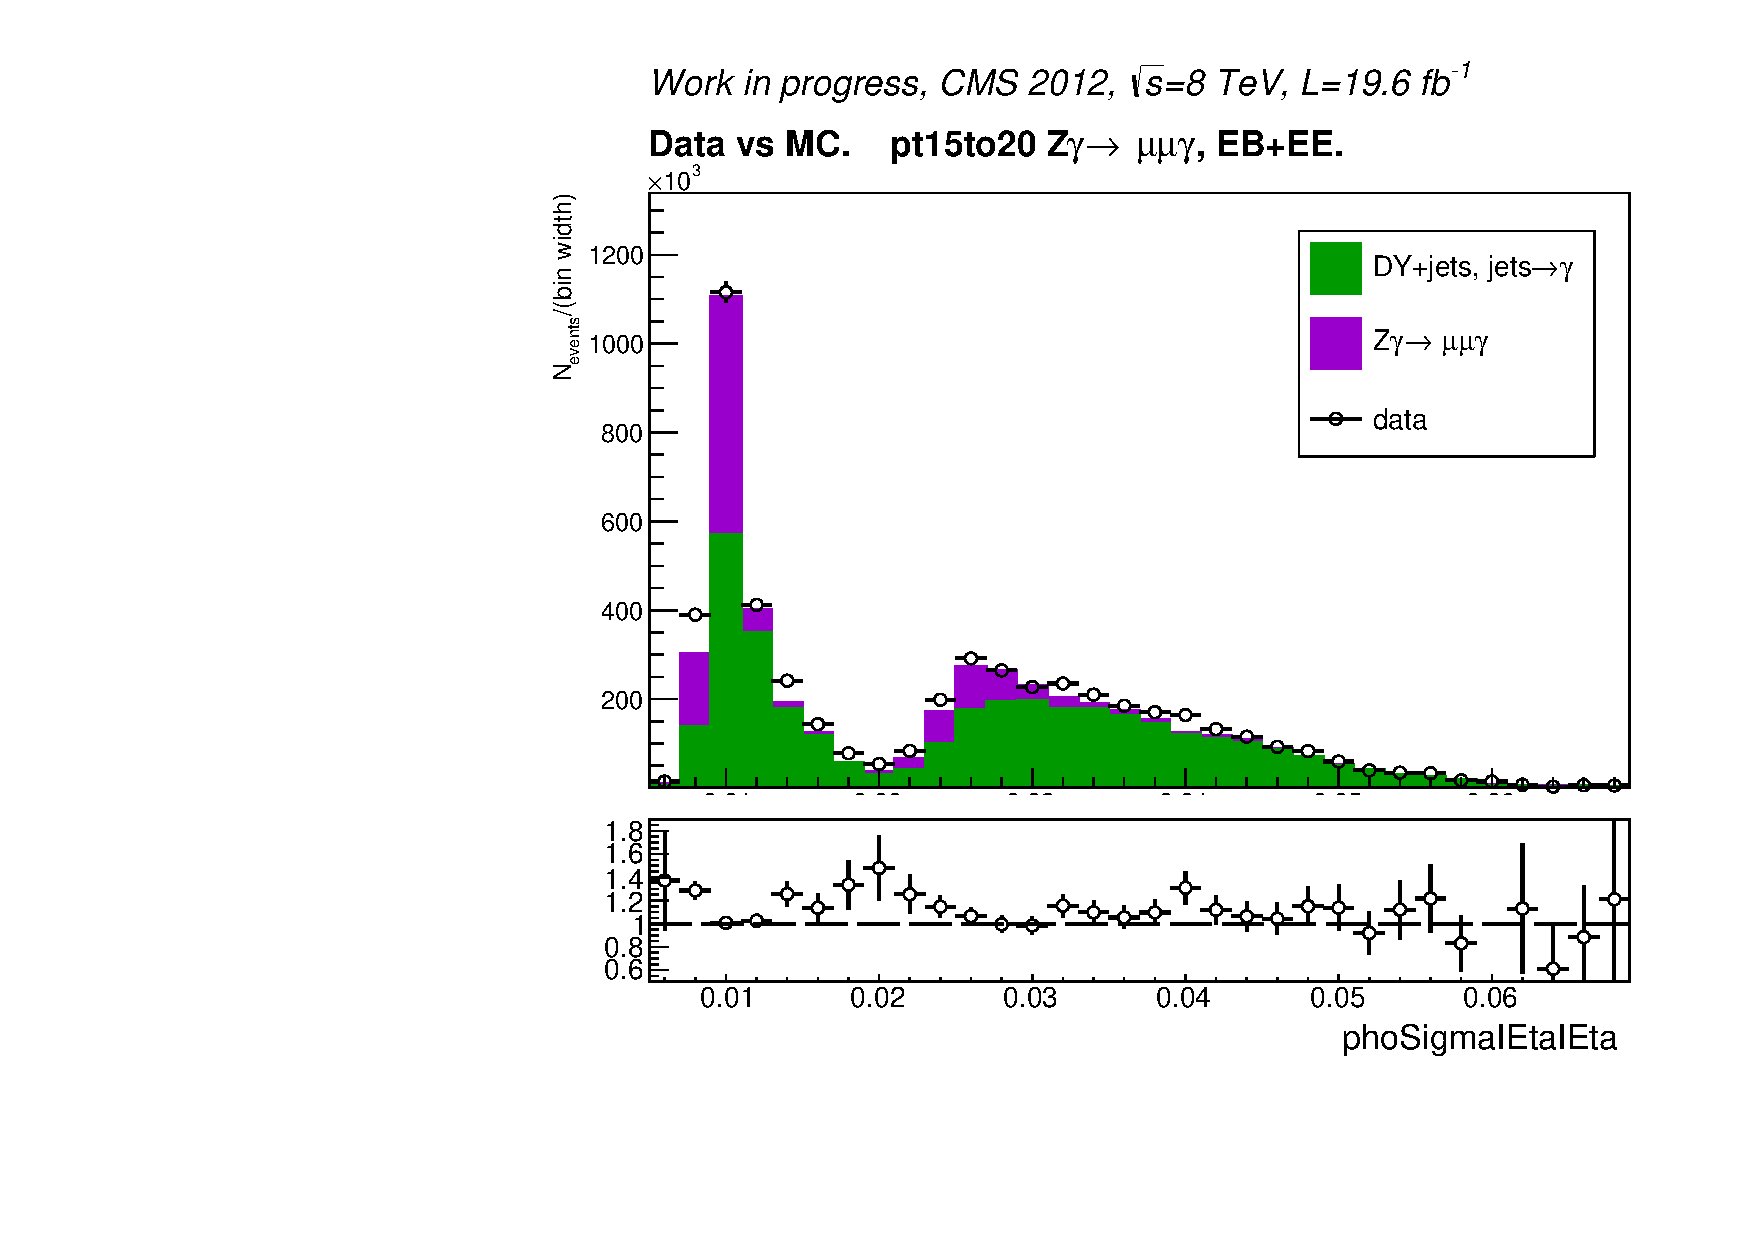
\includegraphics[width=0.45\textwidth]{../figs/figs_v11/MUON_ZGamma/PrepareYields/c_TotalDATAvsMC_EtaCommon__phoSigmaIEtaIEtaFSR_EXCLUDED_pt15to20_.pdf}\\
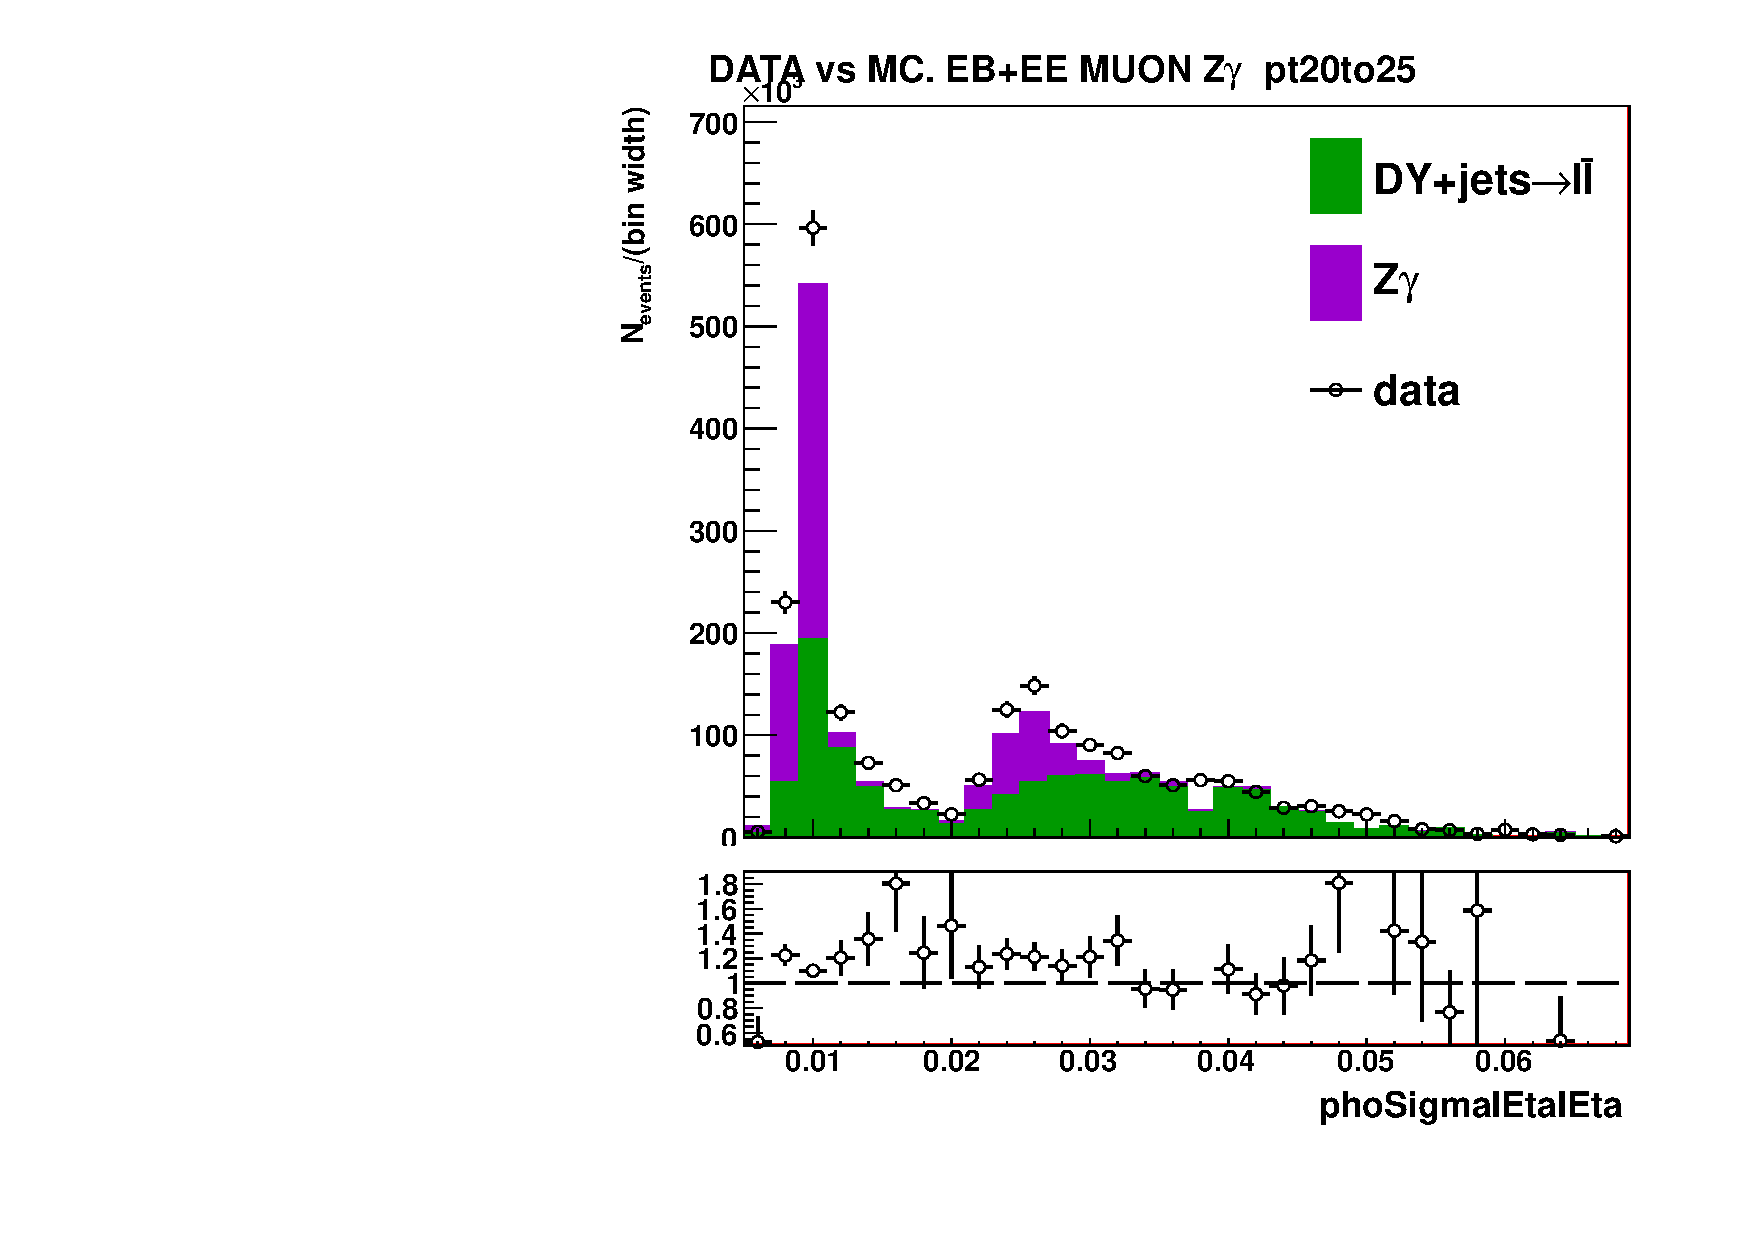
\includegraphics[width=0.32\textwidth]{../figs/figs_v11/MUON_ZGamma/PrepareYields/c_TotalDATAvsMC_EtaCommon__phoSigmaIEtaIEtaFSR_EXCLUDED_pt20to25_.pdf}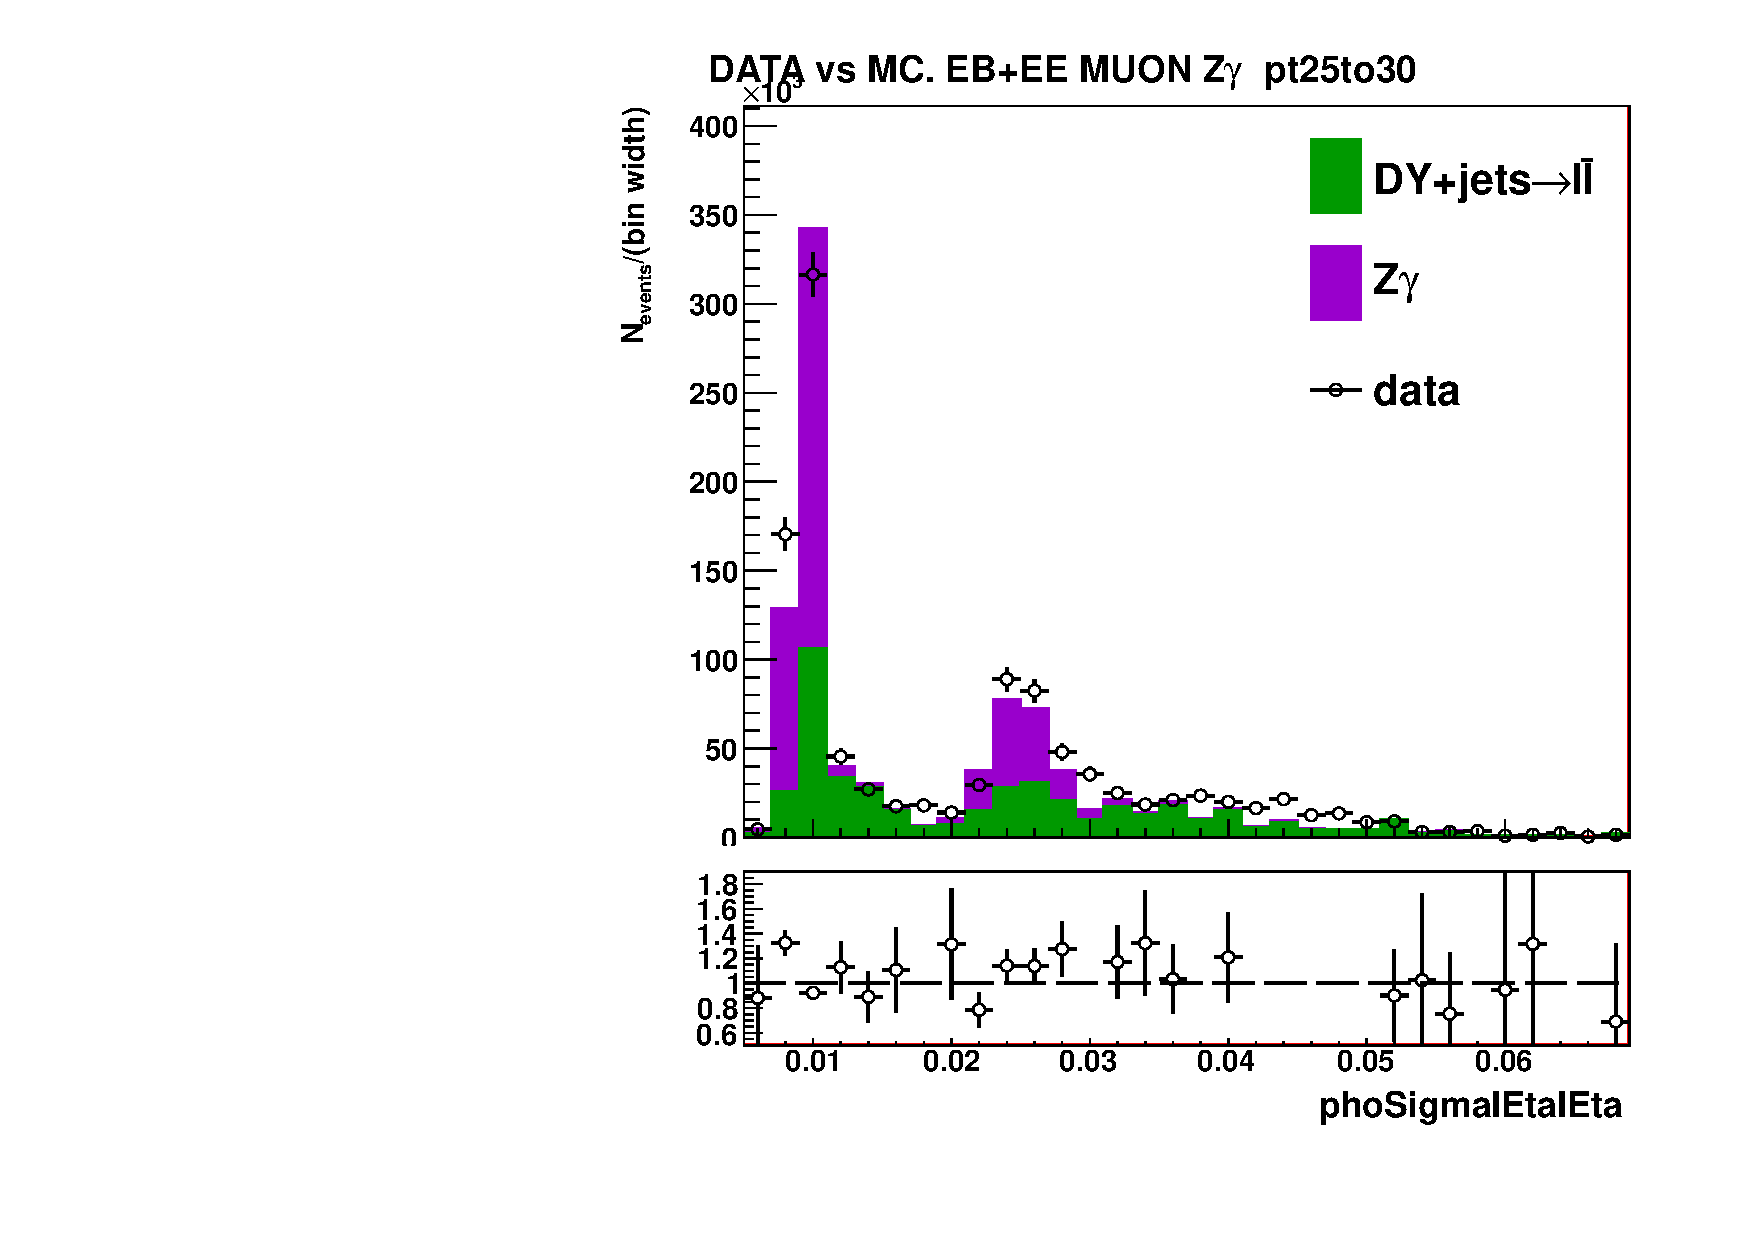
\includegraphics[width=0.32\textwidth]{../figs/figs_v11/MUON_ZGamma/PrepareYields/c_TotalDATAvsMC_EtaCommon__phoSigmaIEtaIEtaFSR_EXCLUDED_pt25to30_.pdf}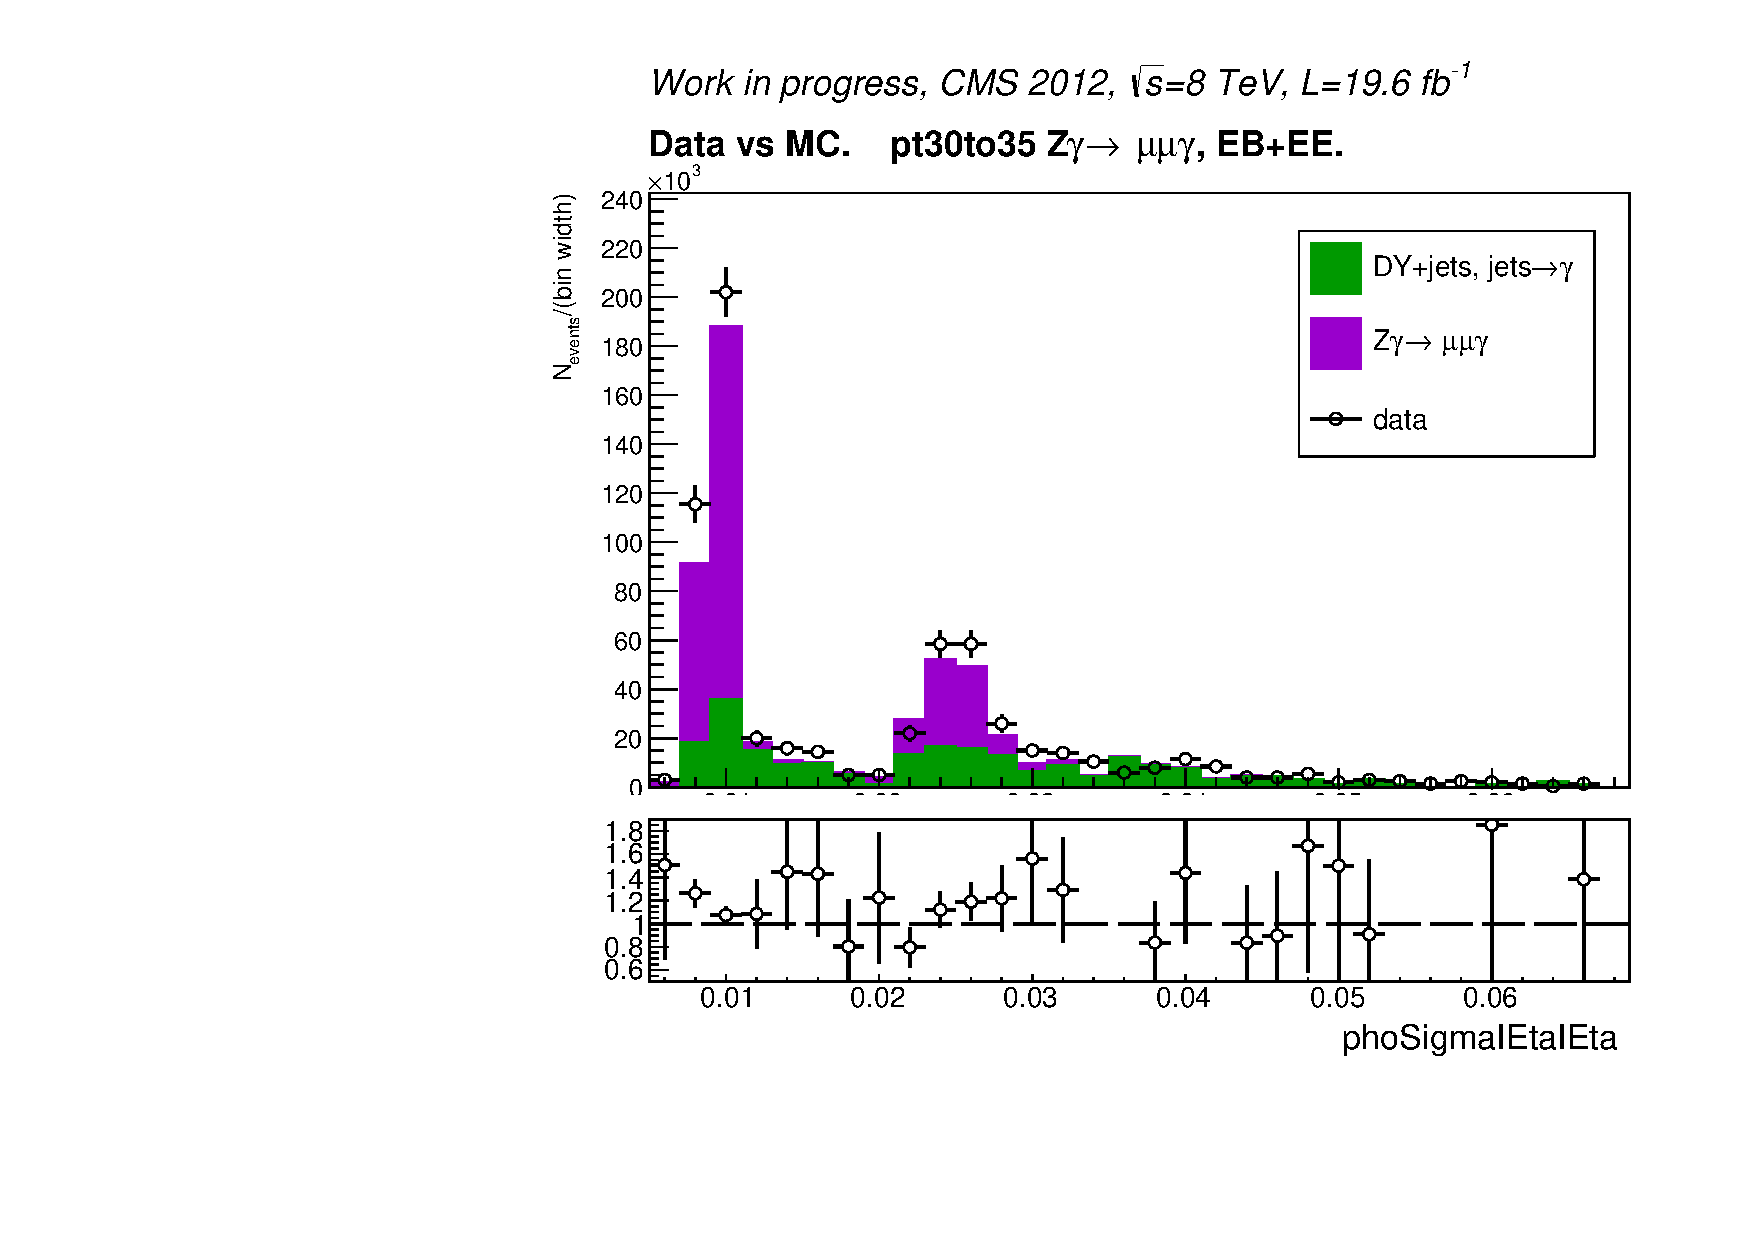
\includegraphics[width=0.32\textwidth]{../figs/figs_v11/MUON_ZGamma/PrepareYields/c_TotalDATAvsMC_EtaCommon__phoSigmaIEtaIEtaFSR_EXCLUDED_pt30to35_.pdf}\\
\includegraphics[width=0.32\textwidth]{../figs/figs_v11/MUON_ZGamma/PrepareYields/c_TotalDATAvsMC_EtaCommon__phoSigmaIEtaIEtaFSR_EXCLUDED_pt35to45_.pdf}\includegraphics[width=0.32\textwidth]{../figs/figs_v11/MUON_ZGamma/PrepareYields/c_TotalDATAvsMC_EtaCommon__phoSigmaIEtaIEtaFSR_EXCLUDED_pt45to55_.pdf}\includegraphics[width=0.32\textwidth]{../figs/figs_v11/MUON_ZGamma/PrepareYields/c_TotalDATAvsMC_EtaCommon__phoSigmaIEtaIEtaFSR_EXCLUDED_pt55to500_.pdf}\\
  \caption{$Z\gamma$-selected ISR events, data vs MC. Distributions of $\sigma_{i\eta i \eta}$ are used for preparing real-$\gamma$ templates. Fake-$\gamma$ contribution to ISR region is subtracted based on DY+jets MC prediction to prepare real-$\gamma$ templates. The templates are prepared separately for barrel and endcap photons.}
  \label{fig:Zg_ISR_phoSigmaIEtaIEta}
  \end{center}
\end{figure}
